\documentclass[12pt,onecolumn,oneside,letterpaper]{article}

% ADD OPTIONS FOR FINAL DRAFT:     12pt, final

\usepackage{amsmath}

\usepackage{unicode-math}

\usepackage{fontspec}
\usepackage{xunicode}
\usepackage{xltxtra}

\setmainfont{Times New Roman}

%%% XITS Math Font
\setmathfont
[    Extension = .otf,
      BoldFont = *bold,
]{xits-math}

%%% STIX Math Font
%\setmathfont{STIX Math}


%%% packages %%%%%%%%%%%%%%%%%%%%%%%%%%%%%%%%%%%%%%%%%%%%%%%%%%%%%%%%%%
\usepackage{calc,bm,textcomp,latexsym,footmisc}
\usepackage{framed,url,verbatim}
\usepackage{longtable,multirow}
\usepackage{subfigure}
\usepackage[hang,small,bf]{caption}
\usepackage{graphicx}
\usepackage[usenames,dvipsnames]{xcolor}
\usepackage[margin=0.7in,top=1in,bottom=1in]{geometry}

\usepackage[backend=biber,texencoding=utf8,bibencoding=utf8,style=numeric-comp,sorting=none]{biblatex}
\addbibresource[datatype=bibtex]{bibliography/clas_general.bib}
\addbibresource[datatype=bibtex]{bibliography/clas_proposals.bib}
\addbibresource[datatype=bibtex]{bibliography/clas_theses.bib}
\addbibresource[datatype=bibtex]{bibliography/pdg.bib}

% placeins package adds \FloatBarrier command to flush figures
% section option puts \FloatBarrier before every section
\usepackage[section]{placeins}

\usepackage[colorlinks]{hyperref}
\definecolor{DarkBlue}{rgb}{0,0.1,0.4}
\hypersetup{
    bookmarksnumbered,
    bookmarksopen=false,
    bookmarksopenlevel=\maxdepth,
    linkcolor=blue,
    urlcolor=DarkBlue,
    citecolor=green
}

%%% allows the use of \index{word!subword!subsubword}
%%%   or \glossary{word} commands in text
%%%   \index{cheese|see{crackers}} for crossreference
%%%   \index{Kraft@\textit{Kraft}} for changing font in index
%\usepackage{makeidx}
    %\makeindex
%%%%%%%%%%%%%%%%%%%%%%%%%%%%%%%%%%%%%%%%%%%%%%%%%%%%%%%%%%%%%%%%%%%%%%%

%%% new commands and macros %%%%%%%%%%%%%%%%%%%%%%%%%%%%%%%%%%%%%%%%%%%
\newlength{\figwidth}
\setlength{\figwidth}{0.9\columnwidth}

\newlength{\qfigheight}
\setlength{\qfigheight}{0.25\textheight}

\newlength{\hfigheight}
\setlength{\hfigheight}{0.5\textheight}

\newcommand{\abbr}[1]{\textsc{\texttt{#1}}}
\newcommand{\desg}[1]{\texttt{#1}}
\newcommand{\prog}[1]{\texttt{#1}}

\newcommand{\todo}[1]{\textbf{\textcolor{Orange}{#1}}}

\def\Lqcd{\mathcal{L}_{\mathtt{QCD}}}
\def\qfield{\psi}
\def\qbarfield{\overline{\psi}}

\newcommand{\bank}[4]{$\mathtt{#1}^{#2}_{#3}\lbrack\mathtt{#4}\rbrack$}

\def\th{\textsuperscript{th}}
\def\ith{i\th}

\def\um{{\textmu}m}
\def\d{\mathrm{d}}

%\def\coloronline{(Color online.)\ }
\def\coloronline{}

%%% quarks
\def\uquark{\mathbf{u}}
\def\dquark{\mathbf{d}}
\def\squark{\mathbf{s}}

%%% particles
\def\photon{\gammaup}
\def\electron{\mathrm{e}^-}
\def\positron{\mathrm{e}^+}
\def\nucleon{\mathrm{N}}
\def\proton{\mathrm{p}}
\def\neutron{\mathrm{n}}
\def\pion{\piup}
\def\kaon{\mathrm{K}}
\def\hyperon{\mathrm{Y}}
\def\etameson{\etaup}
\def\omegameson{\omegaup}
\def\phimeson{\varphiup}
\def\rhomeson{\rhoup}

%%% TAGGER and RF related times
\def\trf{t_{\mathtt{RF}}}
\def\ttag{t_{\mathtt{TAG}}}
\def\ttagrf{t_{\mathtt{TAG,RF}}}
\def\tpho{t_\mathrm{photon}}
\def\tprop{t_\mathrm{prop}}
\def\ttrigoffset{t_{\mathrm{trigger-offset}}}

\def\dtpho{\Delta\tpho}

%%% BEAM energy
\def\ebeam{E_{\mathrm{beam}}}

%%% TOF Energy deposit
\def\etof{\frac{\mathrm{d}E}{\mathrm{d}x}(\mathtt{TOF})}
\def\varetof{\mathrm{d}E/\mathrm{d}x(\mathtt{TOF})}

%%% Beta
\def\betasttof{\beta_\mathtt{ST-TOF}}
\def\betatof{\beta_\mathtt{TOF}}
\def\betapid{\beta_\mathtt{PID}}

%%% path lengths
\def\lst{\ell_{\mathtt{ST}}}
\def\ltof{\ell_{\mathtt{TOF}}}
\def\lsttof{\ell_{\mathtt{ST-TOF}}}

%%% raw subsystem times
\def\tst{t_{\mathtt{ST}}}
\def\ttof{t_{\mathtt{TOF}}}
\def\dtsttof{\Delta t_{\mathrm{ST-TOF}}}

%%% vertex times
\def\tv{t_{\mathrm{vtx}}}
\def\tvtagrf{t_{\mathrm{vtx}}(\mathtt{TAG_{RF}})}
\def\tvtof{t_{\mathrm{vtx}}(\mathtt{TOF})}
\def\tvst{t_{\mathrm{vtx}}(\mathtt{ST})}
\def\tvpid{t_{\mathrm{vtx}}(\mathtt{PID})}

%%% delta vertex times
\def\dtvst{\Delta t_\mathrm{vtx}(\mathtt{TOF-ST})}
\def\dtvpid{\Delta t_\mathrm{vtx}(\mathtt{TOF-PID})}

\def\adcst{\mathtt{ADC}_{\mathtt{ST}}}

\def\M{\mathrm{M}}
\def\MM{\mathrm{MM}}

%%% units
\def\GeV{\mathrm{GeV}}
\def\ns{\mathrm{ns}}

\newcommand{\bra}[1]{\left<#1\right|}
\newcommand{\ket}[1]{\left|#1\right>}
\newcommand{\braket}[2]{\left<#1\middle|#2\right>}

\newcommand*\midhrulefill{%
    \leavevmode\leaders\hrule depth-2pt height 2.4pt\hfill\kern0pt
}


\def\thedraft{0.9}
%\def\excerpt{EXCERPT}
\def\excerpt{}

\author{R.A. Badui \and C. Bookwalter \and S. Chandavar \and P. Eugenio \and J.T. Goetz \and L. Guo \and K. Hicks \and V. Kubarovsky \and M.C. Kunkel \and M. Paolone \and W. Phelps \and M. Saini \and C. Salgado \and D. Schott \and D.P. Weygand}

\title{\desg{g12} Analysis Procedures, Statistics and Systematics}
\def\brieftitle{\desg{g12} Analysis Procedures}
\date{\today}
%%%%%%%%%%%%%%%%%%%%%%%%%%%%%%%%%%%%%%%%%%%%%%%%%%%%%%%%%%%%%%%%%%%%%%%

%%% headers. %%%%%%%%%%%%%%%%%%%%%%%%%%%%%%%%%%%%%%%%%%%%%%%%%%%%%%%%%%
\usepackage{fancyhdr}

\fancypagestyle{headings}{
    \renewcommand{\headheight}{30pt}
    \renewcommand{\headrulewidth}{0pt}
    %%% draft headers %%%%%%%%%%%%%%%%%%%%%%%%%%%%%%%%%%%%%%%%%%%%%%%%%
    \fancyhead[L]{\brieftitle \quad \bf{DRAFT \thedraft} \excerpt}
    \fancyhead[R]{Typeset on \today}
    %%% final headers %%%%%%%%%%%%%%%%%%%%%%%%%%%%%%%%%%%%%%%%%%%%%%%%%
    %\fancyhead[L]{\brieftitle}
    %\fancyhead[R]{\nouppercase{\leftmark}}
}
%%% draft header for plain and empty pages %%%%%%%%%%%%%%%%%%%%%%%%%%%%
\fancypagestyle{plain}{
    \renewcommand{\headheight}{30pt}
    \fancyhead[L]{\brieftitle \quad \bf{DRAFT \thedraft} \excerpt}
    \fancyhead[R]{Typeset on \today}
    \renewcommand{\headrulewidth}{0pt}
}
\fancypagestyle{empty}{
    \renewcommand{\headheight}{30pt}
    \fancyhead[L]{\brieftitle \quad \bf{DRAFT \thedraft} \excerpt}
    \fancyhead[R]{Typeset on \today}
    \renewcommand{\headrulewidth}{0pt}
}
%%%%%%%%%%%%%%%%%%%%%%%%%%%%%%%%%%%%%%%%%%%%%%%%%%%%%%%%%%%%%%%%%%%%%%%

%%% spacing %%%%%%%%%%%%%%%%%%%%%%%%%%%%%%%%%%%%%%%%%%%%%%%%%%%%%%%%%%%
% make titles ragged right and leave the text justified.
\usepackage{sectsty}
    \chapterfont{\raggedright}
    \sectionfont{\raggedright}
    \subsectionfont{\raggedright}
    \subsubsectionfont{\raggedright}

\usepackage{setspace} % allows \<double,onehalf,single>spacing
   \singlespacing
%   \onehalfspacing
%   \doublespacing

%%% line spacing adjustment for the align environment
%%% use this when doublespacing:
%\setlength{\jot}{-0.3em}

\def\figures{figures}

\setlength{\footskip}{0.3in}
%%%%%%%%%%%%%%%%%%%%%%%%%%%%%%%%%%%%%%%%%%%%%%%%%%%%%%%%%%%%%%%%%%%%%%%

\begin{document}

%%% define the footnote symbol. Can be one of these:
    %\fnsymbol   *, + ...
    %\arabic     1, 2 ...
    %\roman      i, ii ...
    %\Roman      I, II ...
    %\alph       a, b ...
    %\Alph       A, B ...
\renewcommand{\thefootnote}{\fnsymbol{footnote}}
%%%%%%%%%%%%%%%%%%%%%%%%%%%%%%%%%%%%%%%%%%%%%%%%%%%%%%%%%%%%%%%%%%%%%%%

\pagestyle{headings}
%\renewcommand{\sectionmark}[1]{\markboth{#1}{}}

\pdfbookmark[1]{Title}{title}
\maketitle

\pdfbookmark[1]{Table of Contents}{toc}
    \tableofcontents \clearpage
%\phantomsection \addcontentsline{toc}{section}{List of Figures}
    %\listoffigures \clearpage
%\phantomsection \addcontentsline{toc}{section}{List of Tables}
    %\listoftables \clearpage

\begin{abstract}
This document serves to summarize all information needed to process and analyze data from the \abbr{CLAS} \desg{g12} experiment taken in the summer of 2008. This was a high-luminosity, high-energy real-photon run with a 65~nA circularly polarized beam, 40~cm unpolarized $\ell$H$_2$ target and an $\Ebeam$ up to 5.7~GeV. The associated proposals, and therefore the trigger, focused on the high-energy part of the tagger, and though it was not part of the original proposals, the Cerenkov was active for most of the run.
\end{abstract}

\section{\label{sec:summary}Summary of Running Conditions}

This document is organized as follows. Section~\ref{sec:summary} has basic information about the \desg{g12} run, including the physics goals. Section~\ref{sec:calib} describes the calibrations; it is quite long and uses standard \abbr{CLAS} procedures. One item of note is that the beam current was high for \abbr{CLAS}, typically about 60 nA. Of course, the background rate goes quadratically with beam current, and so the \desg{g12} data have more background yet the calibration procedures still work. Section~\ref{sec:data} provides the cooking procedures, as well as the momentum and beam-energy corrections. Since \desg{g12} also had a lepton trigger, Section~\ref{sec:data.lepton} gives additional information relevant to the lepton detection using the CC and EC. Section~\ref{sec:flux} has a straight-forward description of the beam flux, using the \prog{gflux} method with the \verb+–c+ option (clock-based DAQ). Section~\ref{sec:sim} provides the procedures for simulations, including all command-line options (some a1c options are specific to BOS files made from simulations). This section also has specific information for \desg{g12}, such as the fiducial cuts and simulations of the \desg{g12} trigger. Finally, Sections~\ref{sec:resonances} and \ref{sec:xsec} together show that the world data on cross sections for at least two reactions (ω meson production and K$^+$ Λ production) agree well with previously reported world data. This gives us confidence that the calibrations, energy corrections, beam flux and simulations are being done correctly.

The goal of this document is to provide a basis for individual analyses of \desg{g12} data to undergo a shortened analysis review. In other words, if the procedures here are followed also in individual analyses, then the review committees can focus on the cuts and systematics specific to the final state of an individual analysis, with confidence that the calibrations, corrections, etc., have already been reviewed.

The \desg{g12} experiment contained several analyses where the main goal was to search for resonances in the multi-particle final state by performing partial wave analysis. These analyses\cite{clas.thesis.bookwalter, clas.thesis.schott} do not require absolute normalization and therefore several steps discussed below were skipped. For a general discussion of the PWA procedure by \desg{g12} Ref.~\cite{pwa.salgado2014}. We do however provide details for analyses that do want this normalization for cross sections and upper limits later in this document.

The \desg{g12} experiment was a high-luminosity, high-energy real-photon run for \abbr{CLAS}. The electron beam current was 60--65~nA on the 40~cm $\ell$H$_2$ target. A total of $26\times 10^8$ triggers were recorded using several of the 12 available trigger bits. The ``production trigger'' required two prongs (start-counter and time-of-flight coincidence) in two different sectors and in coincidence with a tagger hit at or above 3.6~GeV. There was secondary trigger which required three prongs, again in different sectors, regardless of tagger hits. The running conditions are summarized in Table~\ref{tab:runconditions}. There were three proposals associated with this experiment which are listed here:
\begin{itemize}
    \item \href{https://misportal.jlab.org/ul/ul_office/experimentdb/view_experiment_detail.cfm?paperid=PR-04-005}{\fullcite{clas.proposal.hyclas}}
    \item \href{https://misportal.jlab.org/ul/ul_office/experimentdb/view_experiment_detail.cfm?paperid=PR-04-017}{\fullcite{clas.proposal.superg}}
    \item \href{https://misportal.jlab.org/ul/ul_office/experimentdb/view_experiment_detail.cfm?paperid=PR-08-003}{\fullcite{clas.proposal.pion}}
\end{itemize}

In addition to this document, there is a wealth of information to be found in the wiki pages at
\begin{center}
    \url{http://clasweb.jlab.org/rungroups/g12/wiki}
\end{center}
which has served as a repository for all things related to the \desg{g12} experiment. The dissertations associated with this experiment contain a lot of information as well:

\begin{itemize}
    \item \href{http://www.jlab.org/Hall-B/general/thesis/Goetz_thesis.pdf}{\fullcite{clas.thesis.goetz}}
    \item \href{http://www.jlab.org/Hall-B/general/thesis/Bookwalter_thesis.pdf}{\fullcite{clas.thesis.bookwalter}}
    \item \href{http://www.jlab.org/Hall-B/general/thesis/Schott_thesis.pdf}{\fullcite{clas.thesis.schott}}
    \item \href{http://www.jlab.org/Hall-B/general/thesis/MSaini_thesis.pdf}{\fullcite{clas.thesis.saini}}
    \item \href{http://www.jlab.org/Hall-B/general/thesis/Bono_thesis.pdf}{\fullcite{clas.thesis.bono}}
    \item \href{http://www.jlab.org/Hall-B/general/thesis/Kunkel_thesis.pdf}{\fullcite{clas.thesis.kunkel}}
    \item \href{http://www.jlab.org/Hall-B/general/thesis/Chandavar_thesis.pdf}{\fullcite{clas.thesis.chandavar}}
\end{itemize}


\begin{table}[htpb]
\begin{center}

\begin{minipage}{0.8\textwidth}

\caption{\label{tab:runconditions}The running conditions of the \desg{g12} experiment.}
\begin{center}
\begin{tabular}{lc}

\hline \hline

$\ebeam$ of photon & 5.715~GeV \\
Beam Polarization & Circular \\
e$^-$ Current & 60--65~nA \\
Tagger Range & 5\% - 95\% of e$^-$ energy \\
Tagger Trigger Range & 3.6--5.441~GeV \\
Torus Magnet & $\frac{1}{2} B_\mathrm{max}$ (1930~A) \\
Target Length & 40~cm \\
Target Center ($z$ location) & $-90$~cm \\
Target Material & $\ell$H$_2$ \\
Target Polarization & None \\
Start Counter Offset & 0~cm \\
Radiator Thickness & $10^{-4}$~radiation~lengths \\
Collimator Radius & 6.4~mm \\

\hline \hline

\end{tabular}
\end{center}

\end{minipage}

\end{center}
\end{table}


\subsection{\label{sec:summary.trigger}Trigger Configurations}

\begin{center} \color{OliveGreen}
This section is a verbatim excerpt from the dissertation by J.T.\ Goetz\cite{clas.thesis.goetz}.
\end{center}

The \desg{g12} experiment was the first Hall \desg{B} run-period to implement field programmable gate array (\abbr{FPGA}) processors to handle the trigger logic of the \abbr{abbr{CLAS}} detector (see Sec.~\ref{sec:clas.daq}). With this new \abbr{FPGA}-powered triggering system, came the ability to modify the trigger quickly during the experiment. While potentially dangerous --- these changes must be accounted for in total-cross-sectional analyses for example --- this allowed the group to tune the trigger to get the highest possible rate of physical events.

The trigger bits used during the \desg{g12} running period are defined in Tables~\ref{tab:data.trig.conf.1}, \ref{tab:data.trig.conf.2} and \ref{tab:data.trig.conf.3}. They generally consisted of a number of tracks which were the coincidence of any one of the four start counter paddles and any of the 57 time-of-flight paddles in a given sector as discussed in Sec.~\ref{sec:clas.daq}. The hardware and configuration did not allow triggering on two tracks in the same sector because there were only six signals coming from the \abbr{TOF} --- one for each sector. The coincidence of these tracks with the photon tagger, called the ``Master-\abbr{OR},'' is defined in Table~\ref{tab:data.trig.mor}.

\begin{table}
\begin{minipage}{\textwidth}
\begin{center}
\begin{singlespacing}

\caption[Trigger Configuration 1]{\label{tab:data.trig.conf.1}Trigger configuration for \desg{g12} runs from 56363 to 56594 and 56608 to 56647. (\abbr{ST}$\times$\abbr{TOF})$_{i}$ indicates a single \emph{prong} which is a trigger-level track defined as a coincidence between a start counter and time-of-flight hit in the \ith\ sector or any sector if the subscript index, $i$, is not specified. An added $\times$2 or $\times$3 indicates the coincidence of multiple \emph{prongs} which are not in the same sector. \abbr{MORA} and \abbr{MORB} represent coincidences with tagger hits within a certain energy range as specified in Table~\ref{tab:data.trig.mor}.}

\begin{tabular}{cccc}

\hline \hline

\multicolumn{4}{c}{\desg{g12} runs 56363--56594, 56608--56647} \\

\hline

bit & definition & L2 multiplicity & prescale \\

\hline

1 & \abbr{MORA}$\cdot$(\abbr{ST}$\times$\abbr{TOF})$_{1}\cdot$(\abbr{ST}$\times$\abbr{TOF}) & -- & 1 \\
2 & \abbr{MORA}$\cdot$(\abbr{ST}$\times$\abbr{TOF})$_{2}\cdot$(\abbr{ST}$\times$\abbr{TOF}) & -- & 1 \\
3 & \abbr{MORA}$\cdot$(\abbr{ST}$\times$\abbr{TOF})$_{3}\cdot$(\abbr{ST}$\times$\abbr{TOF}) & -- & 1 \\
4 & \abbr{MORA}$\cdot$(\abbr{ST}$\times$\abbr{TOF})$_{4}\cdot$(\abbr{ST}$\times$\abbr{TOF}) & -- & 1 \\
5 & \abbr{MORA}$\cdot$(\abbr{ST}$\times$\abbr{TOF})$_{5}\cdot$(\abbr{ST}$\times$\abbr{TOF}) & -- & 1 \\
6 & \abbr{MORA}$\cdot$(\abbr{ST}$\times$\abbr{TOF})$_{6}\cdot$(\abbr{ST}$\times$\abbr{TOF}) & -- & 1 \\
7 & \abbr{ST}$\times$\abbr{TOF} & -- & 1 \\
8 & \abbr{MORA}$\cdot$(\abbr{ST}$\times$\abbr{TOF})$\times$2 & -- & 1 \\
11\footnote{bit 11 and \abbr{MORB} were included in the trigger starting with run 56519.} & \abbr{MORB}$\cdot$(\abbr{ST}$\times$\abbr{TOF})$\times$2 & -- & 1 \\
12 & (\abbr{ST}$\times$\abbr{TOF})$\times$3 & -- & 1 \\

\hline \hline

\end{tabular}

\end{singlespacing}
\end{center}
\end{minipage}
\end{table}
 % label: tab:data.trig.conf.1

\begin{table}
\begin{minipage}{\textwidth}
\begin{center}
\begin{singlespacing}

\caption[Trigger Configuration 2]{\label{tab:data.trig.conf.2}Trigger configuration for \desg{g12} runs from 56595 to 56607 and 56648 to 57323. (\abbr{EC}$\times$\abbr{CC}) represents a coincidence between the electromagnetic calorimeter and the \v{C}erenkov subsystems within a single sector using the thresholds as described in Table~\ref{tab:data.ecccthresh}. \abbr{ECP} represents the \emph{photon} threshold trigger from the \abbr{EC} as detailed in Fig.~\ref{fig:clas.daq.trigsec}. See Table~\ref{tab:data.trig.conf.1} for other explanatory details.}

\begin{tabular}{cccc}

\hline \hline

\multicolumn{4}{c}{\desg{g12} runs 56595--56607, 56648--57323 } \\

\hline

bit & definition & L2 multiplicity\footnote{Level 2 triggering was turned off on all bits for runs 56605, 56607 and 56647.} & prescale \\

\hline

1 & \abbr{MORA}$\cdot$(\abbr{ST}$\times$\abbr{TOF}) & 1 & 1000/300\footnote{Prescaling for bits 1 and 4 were 1000 for runs prior to 56668 at which point they both were changed to 300.} \\
2 & \abbr{MORA}$\cdot$(\abbr{ST}$\times$\abbr{TOF})$\times$2 & 2/--\footnote{Level 2 triggering of bit 2 was set to 2 for runs prior to 56665 at which point it was turned off.} & 1 \\
3 & \abbr{MORB}$\cdot$(\abbr{ST}$\times$\abbr{TOF})$\times$2 & 2 & 1 \\
4 & \abbr{ST}$\times$\abbr{TOF} & 1 & 1000/300 \\
5 & (\abbr{ST}$\times$\abbr{TOF})$\cdot$\abbr{ECP}$\times$2 & 1 & 1 \\
6 & (\abbr{ST}$\times$\abbr{TOF})$\cdot$(\abbr{EC}$\times$\abbr{CC}) & 2 & 1 \\
7 & \abbr{MORA}$\cdot$(\abbr{ST}$\times$\abbr{TOF})$\cdot$(\abbr{EC}$\times$\abbr{CC}) & -- & 1 \\
8 & \abbr{MORA}$\cdot$(\abbr{ST}$\times$\abbr{TOF})$\times$2 & -- & 1 \\
11 & (\abbr{EC}$\times$\abbr{CC})$\times$2 & -- & 1 \\
12 & (\abbr{ST}$\times$\abbr{TOF})$\times$3 & -- & 1 \\

\hline \hline

\end{tabular}

\end{singlespacing}
\end{center}
\end{minipage}
\end{table}

 % label: tab:data.trig.conf.2

\begin{table}
\begin{minipage}{\textwidth}
\begin{center}
\begin{singlespacing}

\caption[Trigger Configuration for Single-sector Runs]{\label{tab:data.trig.conf.3}Trigger configuration for the single-sector runs of \desg{g12}. Trigger bits 7--12 were not used for these runs. See Table~\ref{tab:data.trig.conf.1} for explanatory details.}

\begin{tabular}{cccc}

\hline \hline

bit & definition & L2 multiplicity & prescale \\

\hline

1 & \abbr{MORA}$\cdot$(\abbr{ST}$\times$\abbr{TOF})$_{1}$ & sector 1 & 1 \\
2 & \abbr{MORA}$\cdot$(\abbr{ST}$\times$\abbr{TOF})$_{2}$ & sector 2 & 1 \\
3 & \abbr{MORA}$\cdot$(\abbr{ST}$\times$\abbr{TOF})$_{3}$ & sector 3 & 1 \\
4 & \abbr{MORA}$\cdot$(\abbr{ST}$\times$\abbr{TOF})$_{4}$ & sector 4 & 1 \\
5 & \abbr{MORA}$\cdot$(\abbr{ST}$\times$\abbr{TOF})$_{5}$ & sector 5 & 1 \\
6 & \abbr{MORA}$\cdot$(\abbr{ST}$\times$\abbr{TOF})$_{6}$ & sector 6 & 1 \\

\hline \hline

\end{tabular}

\end{singlespacing}
\end{center}
\end{minipage}
\end{table}

 % label: tab:data.trig.conf.3

\begin{table}
\begin{center}
\begin{singlespacing}

\caption[Trigger Configuration (Tagger)]{\label{tab:data.trig.mor}Master-\abbr{OR} definitions for \desg{g12}. The \abbr{TDC} counters were used in the trigger and since each of these corresponds to several energy paddles, the energies given here are approximate. $T$-counter number 1 corresponds to the highest energy photon of approximately 5.4~GeV. Both \abbr{MORA} and \abbr{MORB} are referenced in terms of the trigger logic in Tables~\ref{tab:data.trig.conf.1}, \ref{tab:data.trig.conf.2} and \ref{tab:data.trig.conf.3}. The \emph{single-sector} runs are listed in Table~\ref{tab:data.cook.singlesecruns}.}

\begin{tabular}{c|cc|cc}

\hline \hline

          & \multicolumn{2}{c|}{\abbr{MORA}} & \multicolumn{2}{c}{\abbr{MORB}} \\
run range & $T$-counters & energy (GeV)     & $T$-counters & energy (GeV) \\

\hline

56363--56400 & 1--47 & 1.7--5.4 & -- & -- \\
56401--56518 & 1--25 & 3.6--5.4 & -- & -- \\
56519--57323 & 1--19 & 4.4--5.4 & 20--25 & 3.6--4.4 \\

\hline

\emph{single-sector} & 1--31 & 3.0--5.4 & -- & -- \\

\hline \hline

\end{tabular}

\end{singlespacing}
\end{center}
\end{table}
 % label:  tab:data.trig.mor

There were two sets of thresholds for the \abbr{EC} labeled \emph{photon} and \emph{electron}. These labels did not mean photon or electron specifically, but were considered a first-order approximation. The actual particle identification was done much later in the analysis of the reconstructed data. The thresholds for the \abbr{CC} and \abbr{EC} during the \desg{g12} running period are shown in Table~\ref{tab:data.ecccthresh}.

\begin{table}
\begin{center}
\begin{singlespacing}

\caption[\abbr{EC} and \abbr{CC} Trigger Thresholds]{\label{tab:data.ecccthresh}Threshold values for the electromagnetic calorimeter (\abbr{EC}) and \v{C}erenkov counter (\abbr{CC}) during the \desg{g12} running period. \abbr{EC} thresholds are shown as \emph{inner}/\emph{total}, and \abbr{CC} thresholds are shown as \emph{left}/\emph{right}.}

\begin{tabular}{cc|c}

\hline \hline

\multicolumn{2}{c|}{\abbr{EC}} & \multirow{2}{*}{\abbr{CC}} \\

\emph{photon} & \emph{electron} \\


\hline

50/100~mV & 60/80~mV & 20/20~mV \\
150/300~MeV & 180/240~MeV & $\sim$0.4~photo-electrons \\

\hline \hline

\end{tabular}

\end{singlespacing}
\end{center}
\end{table}
 % label: tab:data.ecccthresh

\FloatBarrier

\subsection{\label{sec:summary.runs}Lists of Runs}

The runs for this experiment range from 56855 to 57317 inclusive. The runs that made it into Tables.~\ref{tab:data.cook.prodruns} and \ref{tab:data.cook.singlesecruns} qualified upon success of reconstructing final-state hadrons using the cooking program's default particle identification in coordination with the hand-written notes by the shift takers. Other runs of note include those used specifically for calibration in Table~\ref{tab:data.cook.org.runs} and normalization, zero-field and empty-target runs in Table~\ref{tab:data.calibruns}.

\begin{center}
\begin{singlespacing}
\begin{longtable}{lr|lr|lr}
\caption[Production Run List]{\label{tab:data.cook.prodruns}List of successfully reconstructed production runs and their beam currents in nA.} \\

\hline \hline
\multicolumn{2}{l|}{runs} & \multicolumn{2}{l|}{runs} & \multicolumn{2}{l}{runs} \\
\multicolumn{2}{r|}{current (nA)} & \multicolumn{2}{r|}{current (nA)} & \multicolumn{2}{r}{current (nA)} \\
\hline
\endfirsthead

\multicolumn{6}{l}{\scriptsize continued from previous page.} \\
\hline
\multicolumn{2}{l|}{runs} & \multicolumn{2}{l|}{runs} & \multicolumn{2}{l}{runs} \\
\multicolumn{2}{r|}{current (nA)} & \multicolumn{2}{r|}{current (nA)} & \multicolumn{2}{r}{current (nA)} \\
\hline
\endhead

\hline
\multicolumn{6}{r}{\scriptsize continued on next page.} \\
\endfoot

\hline \hline
\endlastfoot

56363 & 20 & 56605 & 60 & 56900-56908 & 60 \\
56365 & 30 & 56608-56612 & 60 & 56914-56919 & 60 \\
56369 & 30 & 56614-56618 & 60 & 56921-56922 & 60 \\
56384 & 5 & 56620-56628 & 60 & 56923 & 65 \\
56386 & 20 & 56630-56636 & 60 & 56924 & 70 \\
56401 & 50 & 56638-56644 & 60 & 56925 & 80 \\
56403 & 70 & 56646 & 60 & 56926-56930 & 60 \\
56404 & 60 & 56653-56656 & 60 & 56932 & 60 \\
56405 & 50 & 56660-56661 & 60 & 56935-56940 & 60 \\
56406 & 40 & 56665-56670 & 60 & 56948-56956 & 60 \\
56408 & 80 & 56673-56675 & 60 & 56958 & 60 \\
56410 & 90 & 56679-56681 & 60 & 56960-56975 & 60 \\
56420-56422 & 5 & 56683 & 60 & 56977-56980 & 60 \\
56435 & 5 & 56685-56696 & 60 & 56992-56994 & 60 \\
56436 & 15 & 56700-56708 & 60 & 56996-57006 & 60 \\
56441 & 35 & 56710-56724 & 60 & 57008-57017 & 60 \\
56442 & 30 & 56726-56744 & 60 & 57021-57023 & 60 \\
56443 & 20 & 56748-56750 & 60 & 57025-57027 & 60 \\
56445-56450 & 60 & 56751-56768 & 65 & 57030-57032 & 60 \\
56453-56459 & 60 & 56770-56772 & 65 & 57036-57039 & 60 \\
56460-56462 & 70 & 56774-56778 & 65 & 57062-57069 & 60 \\
56465 & 70 & 56780-56784 & 65 & 57071-57073 & 60 \\
56467-56472 & 70 & 56787-56788 & 65 & 57075-57080 & 60 \\
56478-56483 & 70 & 56791-56794 & 65 & 57095-57097 & 60 \\
56485-56487 & 70 & 56798-56802 & 65 & 57100-57103 & 60 \\
56489-56490 & 70 & 56805-56815 & 65 & 57106-57108 & 60 \\
56499 & 70 & 56821-56827 & 65 & 57114-57128 & 60 \\
56501 & 60 & 56831-56834 & 65 & 57130-57152 & 60 \\
56503 & 57 & 56838-56839 & 65 & 57159-57168 & 60 \\
56504 & 56 & 56841-56845 & 65 & 57170-57185 & 60 \\
56505-56506 & 40 & 56849 & 65 & 57189-57229 & 60 \\
56508-56510 & 60 & 56853-56862 & 65 & 57233-57236 & 60 \\
56513-56517 & 60 & 56864 & 65 & 57249-57253 & 60 \\
56519 & 60 & 56865-56866 & 60 & 57255-57258 & 60 \\
56521-56542 & 60 & 56870 & 65 & 57260-57268 & 60 \\
56545-56550 & 60 & 56874-56875 & 60 & 57270-57288 & 60 \\
56555-56556 & 60 & 56877 & 60 & 57290-57291 & 60 \\
56561-56564 & 60 & 56879 & 60 & 57293-57312 & 60 \\
56573-56583 & 60 & 56897-56898 & 60 & 57317 & 60 \\
56586-56593 & 60 & 56899 & 65 & & \\

\end{longtable}
\end{singlespacing}
\end{center}
 % label:  tab:data.cook.prodruns

\begin{table}
\begin{minipage}{\textwidth}
\begin{center}
\begin{singlespacing}

\caption[Single-sector Run List]{\label{tab:data.cook.singlesecruns}A list of the single-sector runs using the trigger configuration described in Table~\ref{tab:data.trig.conf.3}.}

\begin{tabular}{lr|lr}

\hline \hline
run & current (nA) & run & current (nA) \\
\hline

56476 & 24 & 56910 & 35 \\
56502 & 24 & 56911 & 30 \\
56520 & 24 & 56912 & 25 \\
56544 & 24 & 56913 & 24 \\
56559 & 24 & 56933-4 & 24 \\
56585 & 24 & 56981-3\footnote{\label{foot:no_l2}No Level-2 trigger was used for runs 56981-56985} & 24 \\
56619 & 24 & 56985\footref{foot:no_l2} & 15 \\
56637 & 24 & 56986 & 15 \\
56663-4 & 24 & 56989 & 24 \\
56697 & 24 & 57028 & 24 \\
56725 & 24 & 57061 & 24 \\
56747 & 24 & 57094\footnote{A shorter \abbr{ST} \abbr{ADC} gate was implemented starting with run 57094.} & 24 \\
56769 & 24 & 57129 & 24 \\
56804 & 24 & 57155-6 & 24 \\
56835 & 24 & 57237-8 & 24 \\
56869 & 5 \\

\hline \hline

\end{tabular}

\end{singlespacing}
\end{center}
\end{minipage}
\end{table}
 % tab:data.cook.singlesecruns

\begin{center}
\begin{singlespacing}
\begin{longtable}{ccp{10em}}
\caption[Calibration Run List]{\label{tab:data.cook.org.runs}A list of the runs which were calibrated for the subsystems: tagger (\abbr{TAG}), start counter (\abbr{ST}), and time-of-flight (\abbr{TOF}). The calibrations were comitted into the database for the range starting with the run shown and ending with the run just prior to the next listed run. A brief reason for calibration is given in the last column.} \\

\hline \hline
run & systems affected & reason \\
\hline
\endfirsthead

\multicolumn{3}{l}{\scriptsize continued from previous page.} \\
\hline
run & systems affected & reason\\
\hline
\endhead

\hline
\multicolumn{3}{r}{\scriptsize continued on next page.} \\
\endfoot

\hline \hline
\endlastfoot

56363 & \abbr{TAG, ST, TOF} & start of run \\
56503 & \abbr{ST} & \abbr{ST} adjustment \\
56508 & " & \quad " \quad " \\
56661 & \abbr{TAG, ST, TOF} & trigger and \abbr{ST} changes \\
56663 & " & \quad " \quad " \\
56665 & " & \quad " \quad " \\
56666 & " & \quad " \quad " \\
56670 & \abbr{TAG} & vacuum problem in tagger fixed \\
56673 & \abbr{TAG, ST, TOF} & trigger change \\
56732 & " & \abbr{RF} related problems fixed by Accelerator group \\
56765 & \abbr{TAG} & T20 left \abbr{HV} problem \\
56766 & " & T20 left \abbr{HV} adjusted \\
56782 & \abbr{TAG, ST, TOF} & changes in calibration database \\
56855 & " & \quad " \quad " \\
56923 & " & start of intensity studies \\
57094 & " & changes in calibration database \\
57154 & \abbr{ST} & adjusted \abbr{ST} \abbr{ADC} timing in gate \\

\end{longtable}
\end{singlespacing}
\end{center}
 % tab:data.cook.org.runs

\begin{center}
\begin{singlespacing}
\begin{longtable}{ccl}
\caption[\desg{g12} Special Run List]{\label{tab:data.calibruns}List of special calibration runs done during the \desg{g12} experiment.} \\

\hline \hline
run & current (nA) & description \\
\hline
\endfirsthead

\multicolumn{3}{l}{\scriptsize continued from previous page.} \\
\hline
run & current (nA) & description \\
\hline
\endhead

\hline
\multicolumn{3}{r}{\scriptsize continued on next page.} \\
\endfoot

\hline \hline
\endlastfoot

56397 & 0.05 & normalization \\
56475 & 10 & zero-field \\
56511 & 0.05 & normalization, tagger \abbr{TDC}-left \\
56512 & 0.05 & normalization, tagger \abbr{TDC}-right \\
56584 & 0.05 & normalization \\
56682 & 0.05 & normalization \\
56790 & 0.05 & normalization \\
56931 & 0.05 & normalization \\
56947 & 0.05 & normalization \\
57169 & 0.05 & normalization \\
57239 & 24 & empty-target, single-sector \\
57241 & 80 & empty-target, production \\
57248 & 0.05 & normalization

\end{longtable}
\end{singlespacing}
\end{center}
 % tab:data.calibruns

A script named ``g12runs'' was created to provide a list of the runs which were fully reconstructed without errors. It can also provide a lot of information about each run including the beam current, the number of good scalar intervals, and the run type such as production, calibration, or single-sector. The script resides in the \emph{clasg12} user's home directory here:
\begin{align}
    \texttt{/home/clasg12/local/scripts/g12runs} \nonumber
\end{align}
and has an extensive help message with the ``-h'' as shown here:

\begin{verbatim}
>/home/clasg12/local/scripts/g12runs -h
Usage:     usage: g12runs [options]

    example to get all good data runs:
        g12runs -t prod -t single -x calib

    to get all data runs (prod and single) that have
    been completely cooked, sorted and have complete
    flux information:
        g12runs -t pass1 -t flux -i

Options:
  -h, --help            show this help message and exit
  -r RANGE, --range=RANGE
                        range of runs to print out (inclusive from:to) To get
                        the six-digit run numbers, use this range:
                        557313:557316. Can also be a single run number.
                        default: 56363:557316
  -c CURRENT, --current=CURRENT
                        range of currents to print out (inclusive from:to).
                        examples: 40:80, 20:35 default: 0:90
  -t RUNTYPE, --run-type=RUNTYPE
                        Type of runs to print out. can be any of the
                        following, and may be specified more than once: prod
                        single calib cc dc norm pass1 flux Note: calib
                        includes all norm runs. Use prod, single and calib to
                        get all runs. default: prod, single
  -x EXCLUDE, --exclude-type=EXCLUDE
                        excludes types from being printed out. may be
                        specified more than once.
  -i, --intersect       require all run types specified with the -t option to
                        be valid. Note: "g12runs -tprod -tsingle -i" will
                        result in no output since prod and single run types
                        are mutualy exclusive. Typical usage is to get runs
                        that have complete pass1 and flux data: "g12runs
                        -tpass1 -tflux -i".
  -e, --extra-info      print extra information for each run.
  -m, --max-ind         print maximum index for each run printed.
  -n, --nfiles          print number of files for each run printed.
  -s SET, --set=SET     print runs which correspond to one (or all by default)
                        of ten groups: 1 - 10. These groups represent
                        approximately 10% of the whole run period.
  -a, --scalar          Print out the number of scalar intervals in the form:
                        good/total.
  -d, --dump            Dump all info about all runs.
\end{verbatim}


\section{\label{sec:calib}Calibration and Detector Performance}

The calibration of the raw data was done through seven incomplete but representative passes labeled \verb+pass0_v1+ through \verb+pass0_v7+ though only the last three of these is still available via JLab's mass storage system (\abbr{mss}). All calibration constants were put into the \mbox{\texttt{calib\_user.RunIndexg12}} run index with the exception of certain lepton-specific numbers as discussed in Sec.~\ref{sec:data.lepton}.

\subsection{\label{sec:calib.trig.eff}Trigger Efficiency}

\begin{center} \color{OliveGreen}
This section is a verbatim excerpt from the dissertation by J.T.\ Goetz\cite{clas.thesis.goetz}.
\end{center}

In the first few weeks of \desg{g12}, during ``commissioning,'' an attempt to determine the efficiency of the two-track trigger (bit 8 in Tables.~\ref{tab:data.trig.conf.1} and \ref{tab:data.trig.conf.2}) was made. The rate of this main production trigger rose quadratically with the beam current while the physical event rate increased linearly. The number of accidentals, which must be cut from any analysis, increased with increasing current and at a certain point, the majority of the events taken were accidentals. The trigger rate as a function of the beam current is shown in Fig.~\ref{fig:data.trig.eff}. An estimate of the linear part of the trigger rate shows that approximately 60\% of the events recorded during the \desg{g12} experiment (which ran at 60--65~nA beam current) were accidentals.

\begin{figure}\begin{center}
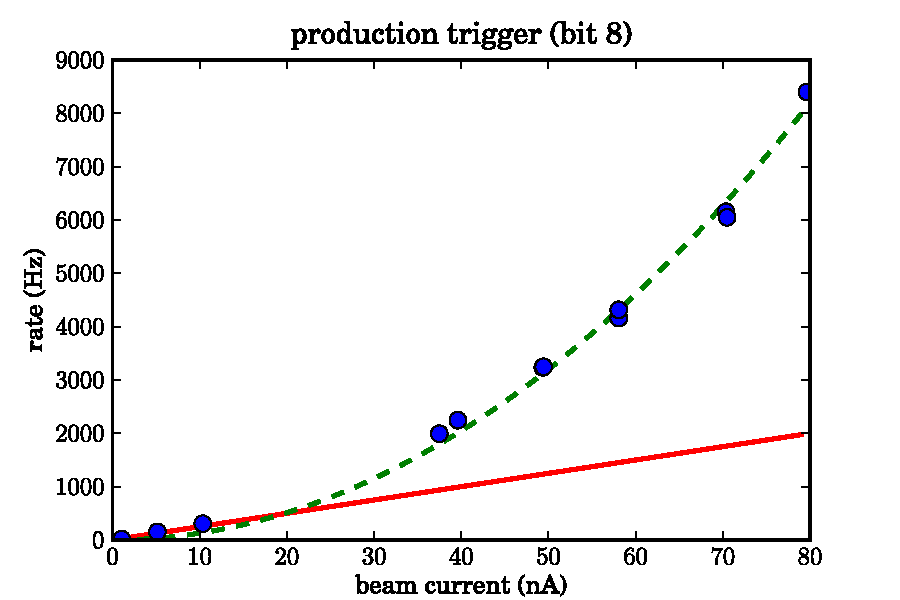
\includegraphics[width=0.6\columnwidth]{figures/calib/trig/trigger_study.eps}
\caption[Trigger Rate vs. Beam Current]{\label{fig:data.trig.eff}The production trigger rate (bit 8 in Tables~\ref{tab:data.trig.conf.1} and \ref{tab:data.trig.conf.2}) was measured for various beam currents shown by the blue dots. The rates below 10~nA are roughly linear and are extrapolated via the red solid line to show an estimate of the physical event rate. The actual trigger rate is fitted with a quadratic shown by the green dashed line. By this estimate, the accidental rate is shown to equal the physical event rate at approximately 40~nA. The \desg{g12} experiment was done at 60--65~nA.}
\end{center}\end{figure}

\FloatBarrier

\subsection{\label{sec:calib.tag}Tagger Timing Calibration}
The timing calibration of the tagger system was performed using the standard procedures. Overall, the quality of the calibration is excellent, showing an overall timing resolution of about $130~ps$, when the tagger time is compared with the RF time. The counter-by-counter alignment can be seen on Fig.~\ref{tagtpho}. The calibration was checked on a run by run basis (Fig.~\ref{tagRun}), and new constants were commissioned when major changes were noticed.

\begin{figure}[htpb]
\begin{center}
 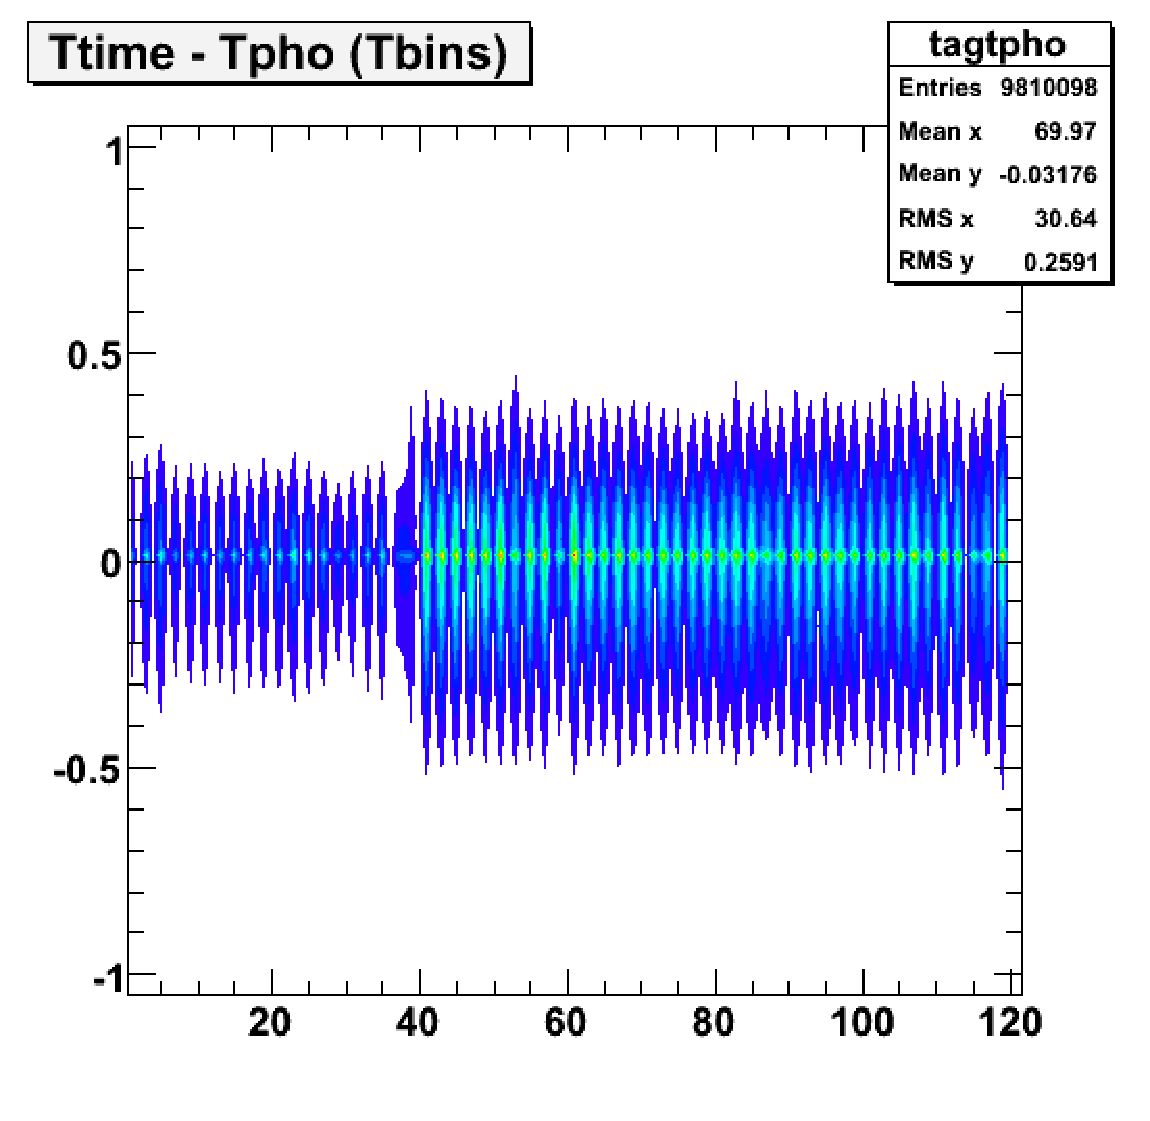
\includegraphics[width=0.45\textwidth]{figures/calib/tag/timing/tagtpho.eps}
  \caption{And example of the tagger timing calibration and the T-counter alignment, comparing  the difference between photon time determined from the tagger elements (T-counters, in this particular plot), and photon timing according to the RF. The relative intensity of the paddles shown are due to the trigger configuration, see Tables.~\ref{tab:data.trig.conf.2} and \ref{tab:data.trig.mor}.}
  \label{tagtpho}
  \end{center}
\end{figure}


\begin{figure}[htpb]
\begin{center}
 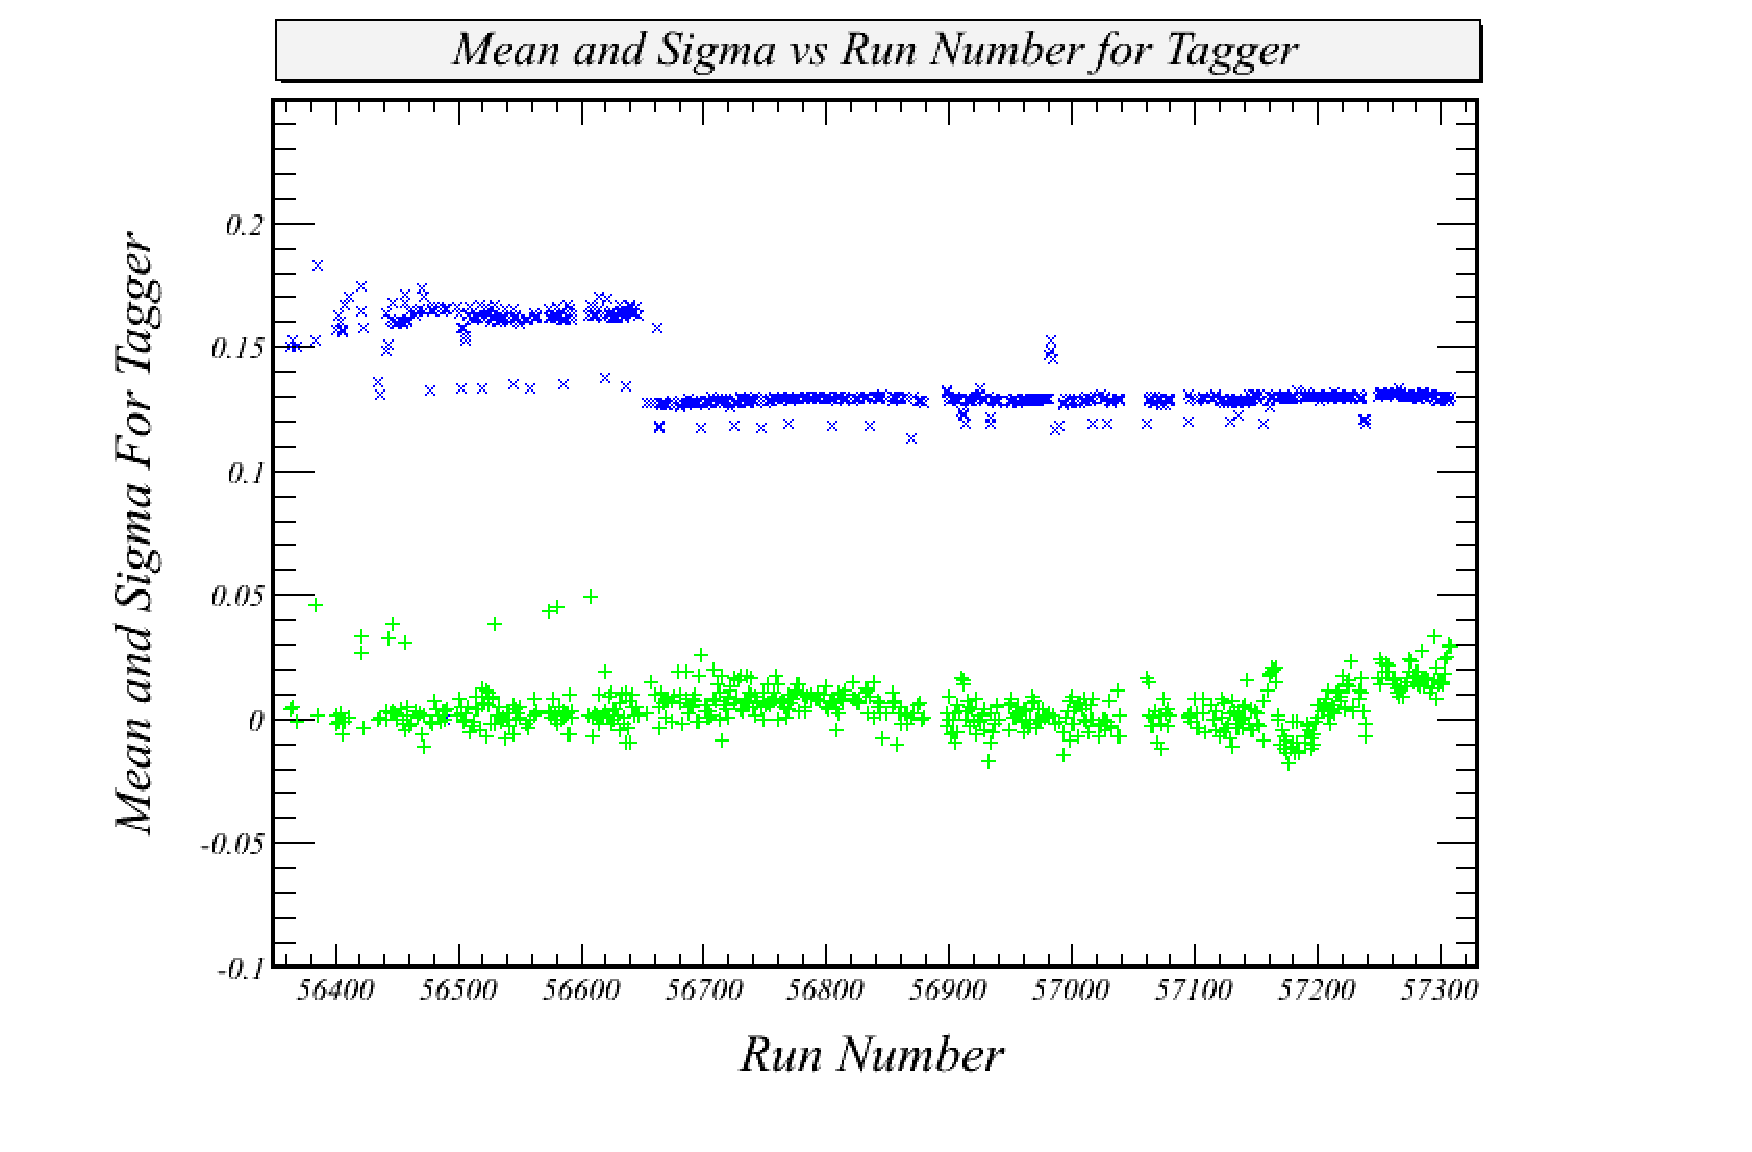
\includegraphics[width=0.45\textwidth]{figures/calib/tag/timing/tagRun.eps}
  \caption{The run-by-run behavior of the tagger timing calibration where the mean is in green and the sigma is in blue. Overall, the tagger timing resolution is about $130~ps$ for the production runs, and the mean behaves stably throughout the running period.}
  \label{tagRun}
  \end{center}
\end{figure}

\subsection{\label{sec:calib.beampol}Beam Polarization}

\subsection{\label{sec:calib.st}Start Counter Calibration and Resolution}

The start counter time-walk calibration took into account the varying geometry of the paddles. Fig.~\ref{fig:calib.st.adcuncor} shows the uncorrected timing difference for paddle 3 (of 24) as a function of \abbr{ADC} while Fig.~\ref{fig:calib.st.adccor} shows the corrected timing. This was done for each paddle and the resulting resolutions can be seen in Fig.~\ref{fig:calib.st.timepion} for pions, Fig.~\ref{fig:calib.st.timeproton} for protons, Fig.~\ref{fig:calib.st.timepion2d} for pions and all paddles, Fig.~\ref{fig:calib.st.timepion.ebeam} for pions a function of beam energy and Fig.~\ref{fig:calib.st.timepion.region} for pions as a function of geometry. The run-by-run resolution can be seen in Fig.~\ref{fig:calib.st.runbyrun}. This shows that the start counter was calibrated properly.

% ADC Uncorrected
\begin{figure}[htbp]\begin{center}
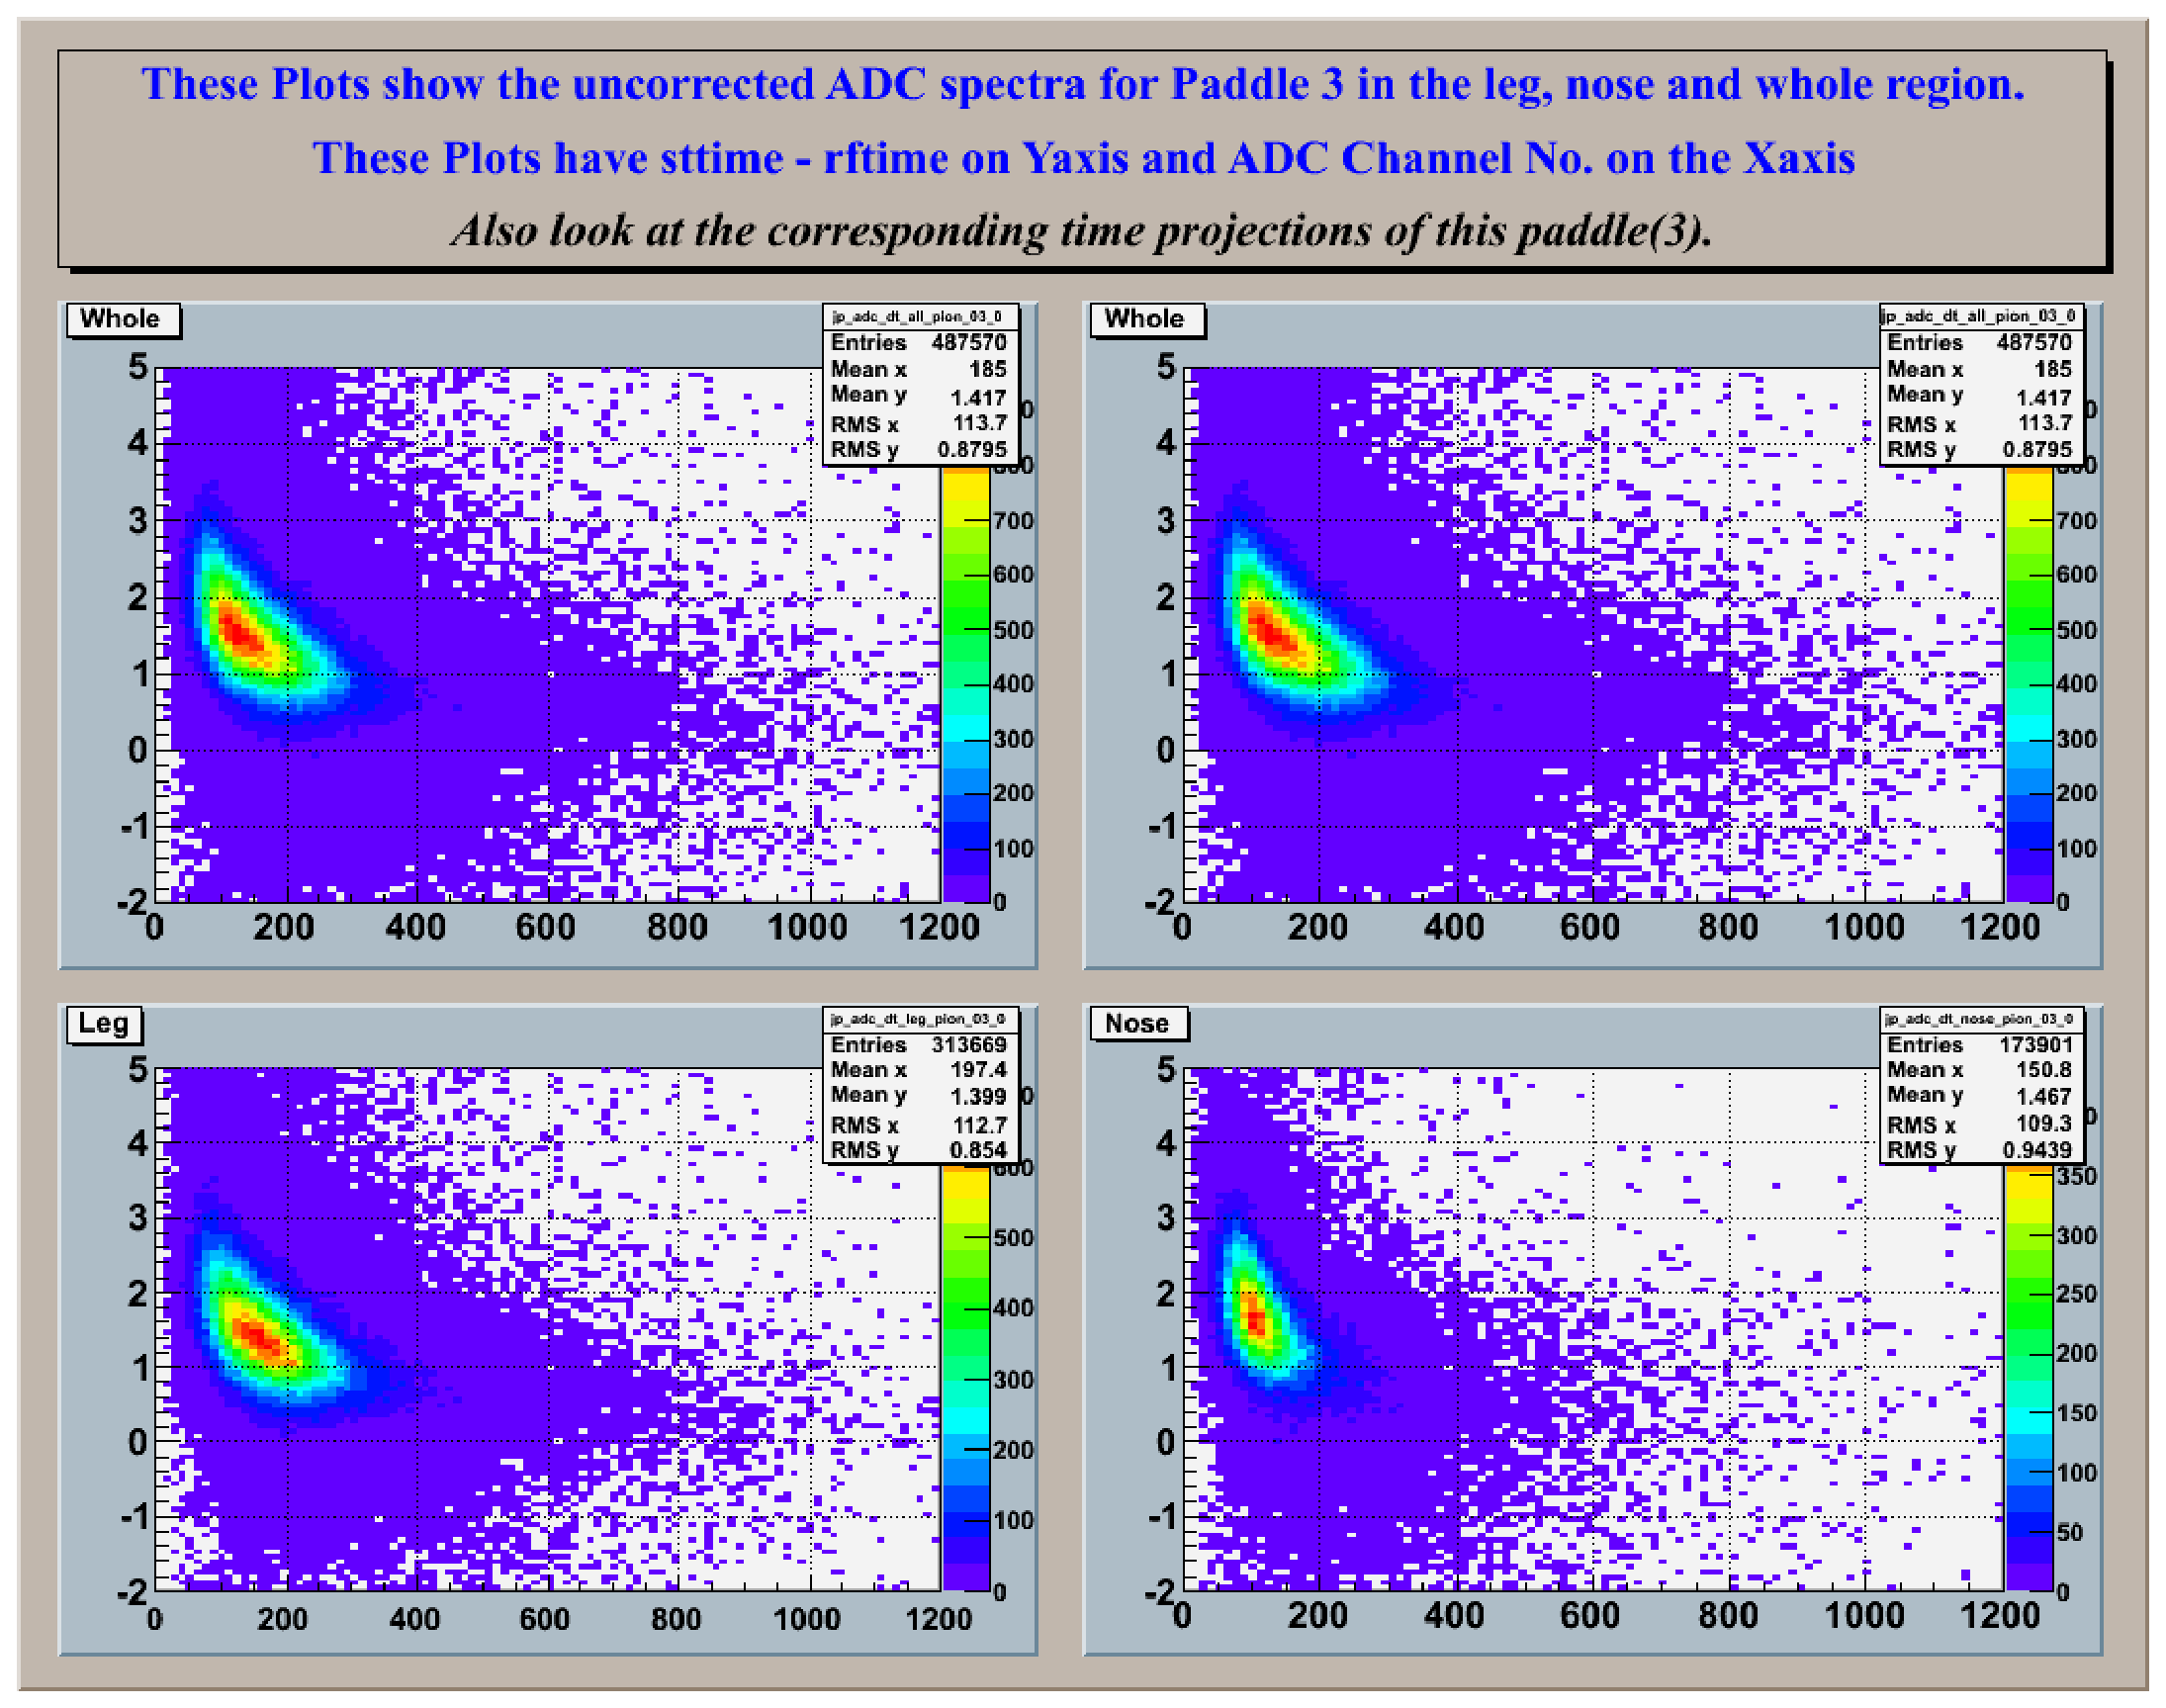
\includegraphics[width=0.65\columnwidth]{figures/calib/st/Uncorrected_adc.eps}
\caption[]{\label{fig:calib.st.adcuncor}ADC spectra for a paddle in the start counter. The top two plots are identical and show the all hits in the paddle. The bottom left plot shows hits in the ``leg'' of the counter and the bottom right shows hits in the ``nose.''}
\end{center}\end{figure}

% ADC Corrected
\begin{figure}[htbp]\begin{center}
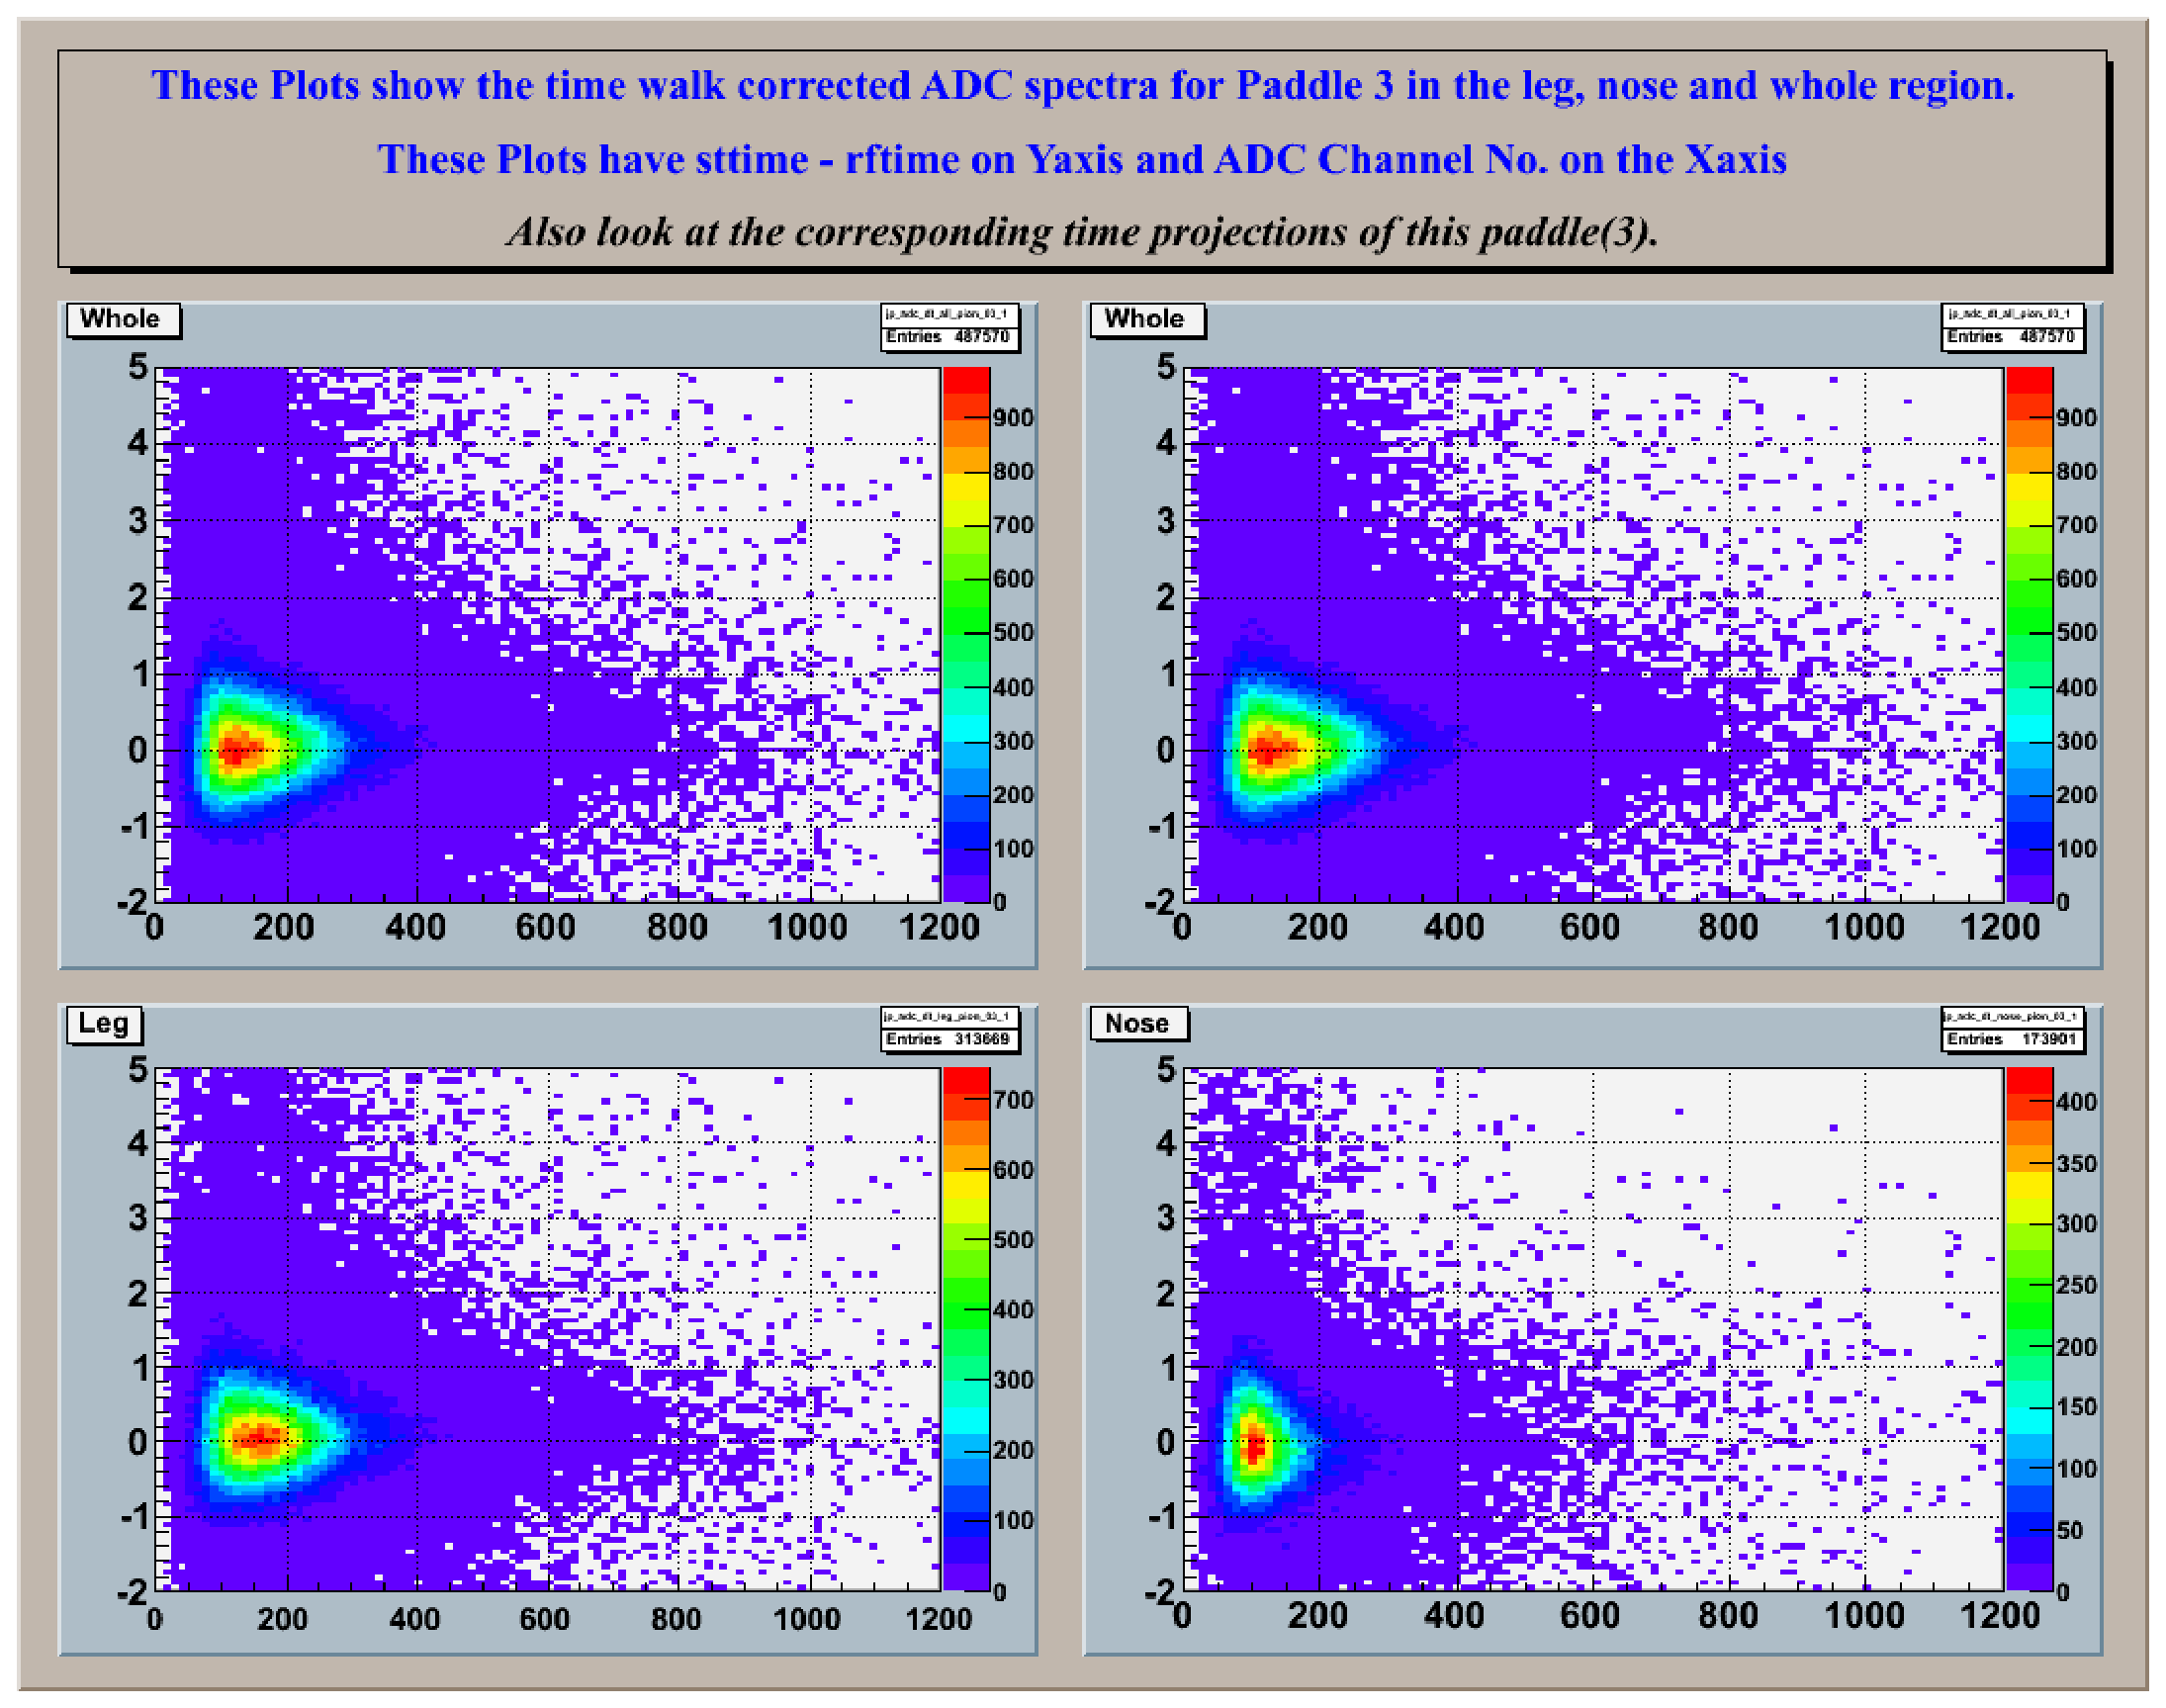
\includegraphics[width=0.65\columnwidth]{figures/calib/st/Corrected_adc.eps}
\caption[]{\label{fig:calib.st.adccor}See caption above and caption in Fig.~\ref{fig:calib.st.adcuncor}.}
\end{center}\end{figure}

\begin{figure}[htbp]\begin{center}
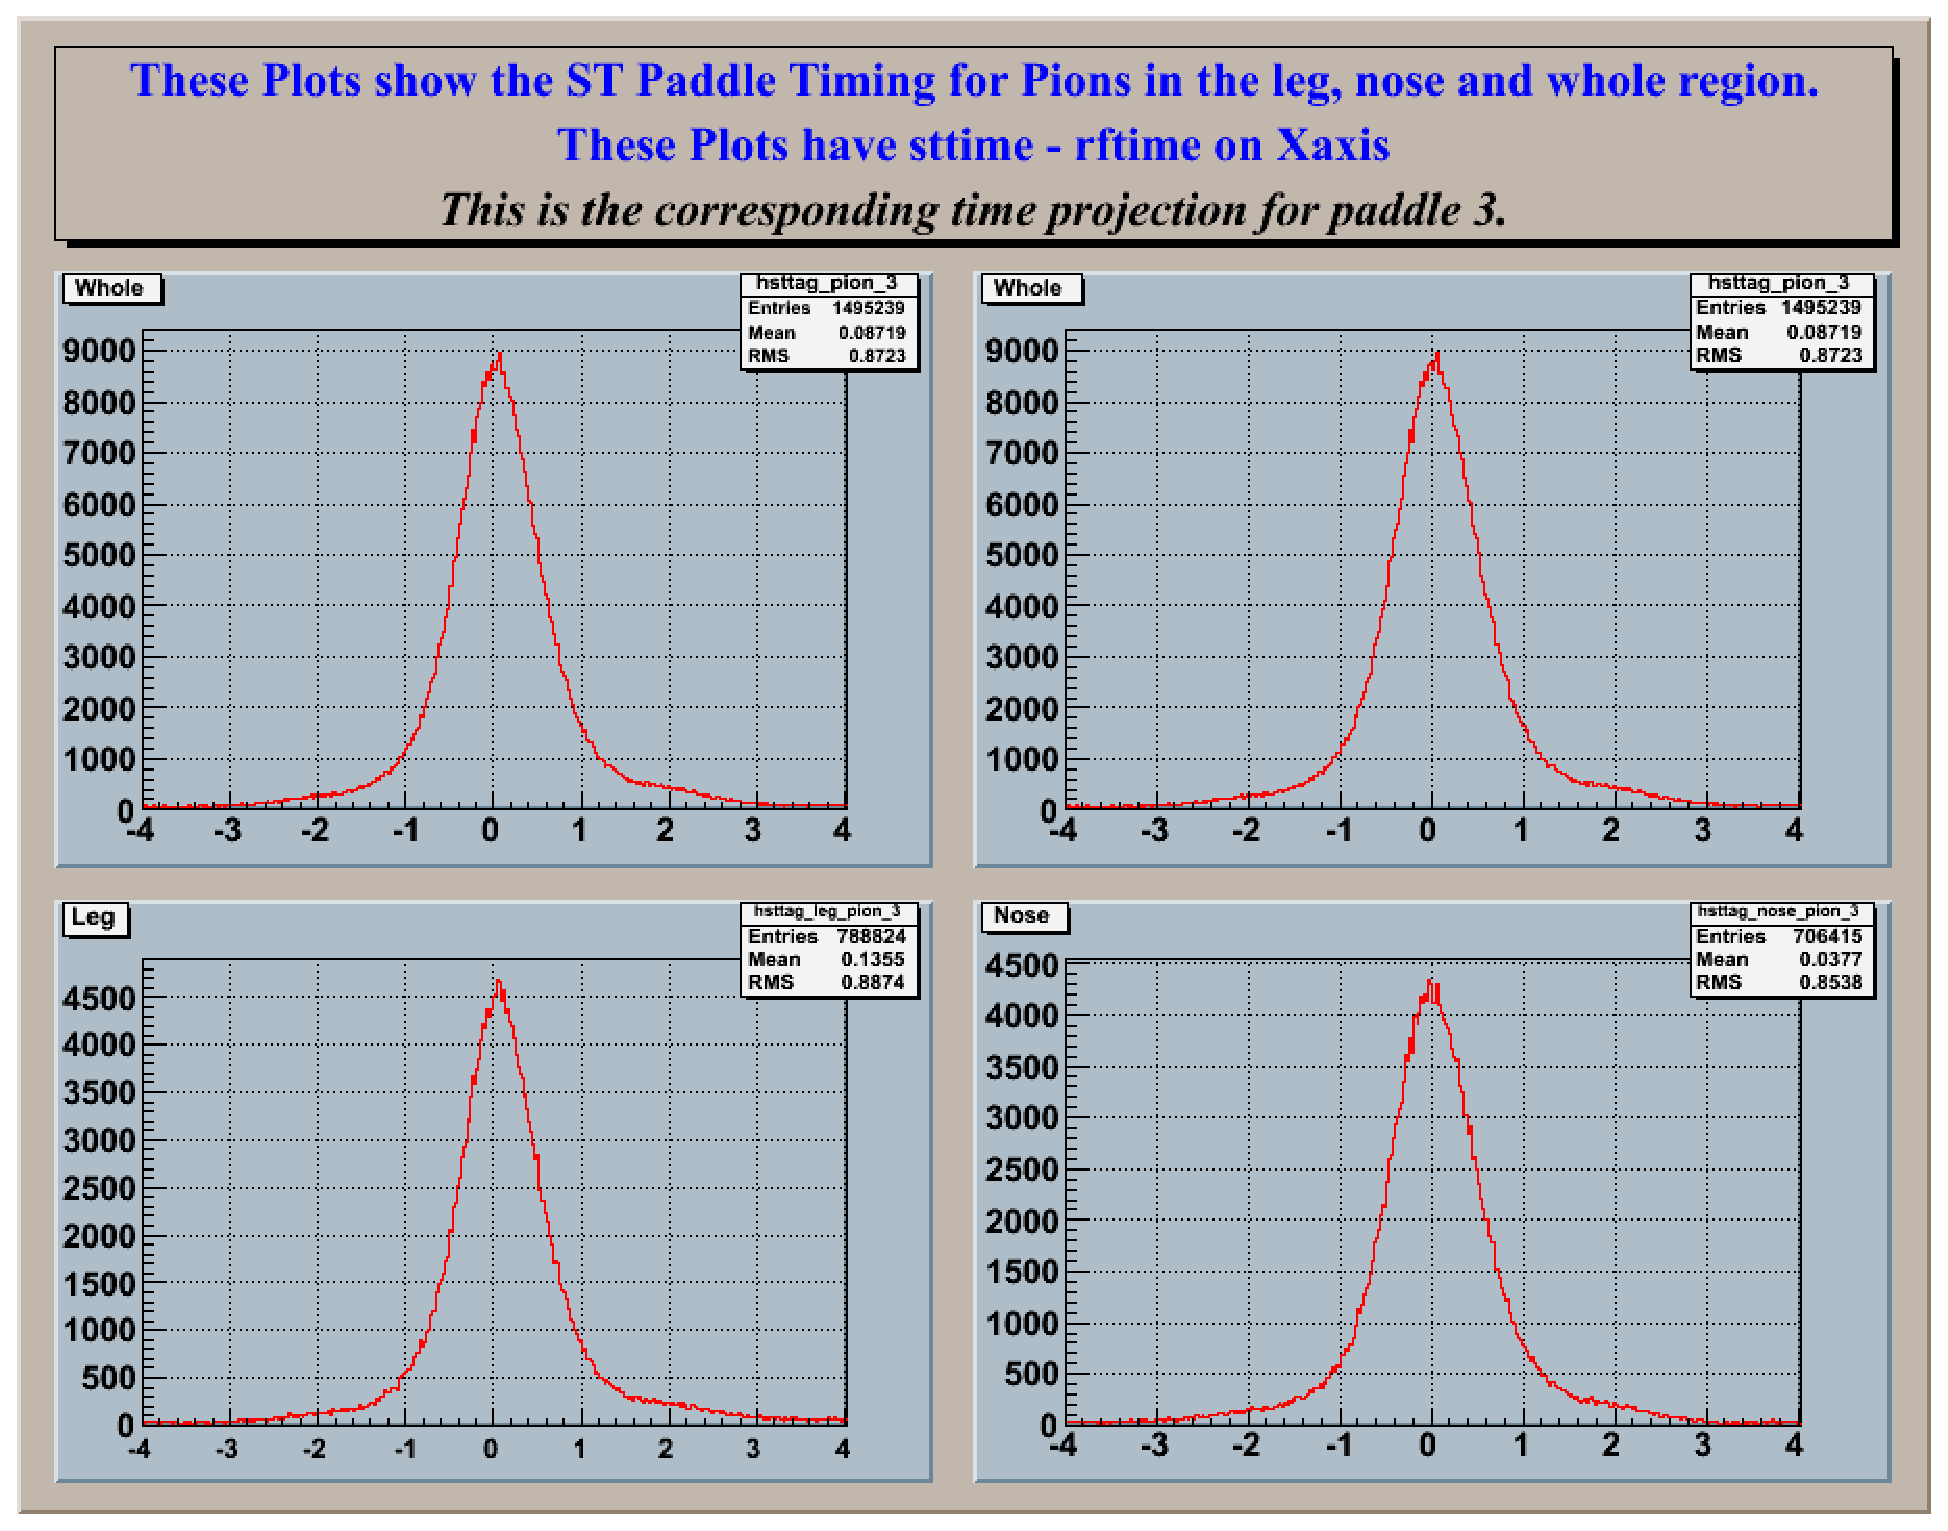
\includegraphics[width=0.65\columnwidth]{figures/calib/st/Hpad3_sttag_pion.eps}
\caption[]{\label{fig:calib.st.timepion}Difference of timing in a paddle of the start counter and the RF time for pions. The top two plots are identical and show the all hits in the paddle. The bottom left plot shows hits in the ``leg'' of the counter and the bottom right shows hits in the ``nose.''}
\end{center}\end{figure}

\begin{figure}[htbp]\begin{center}
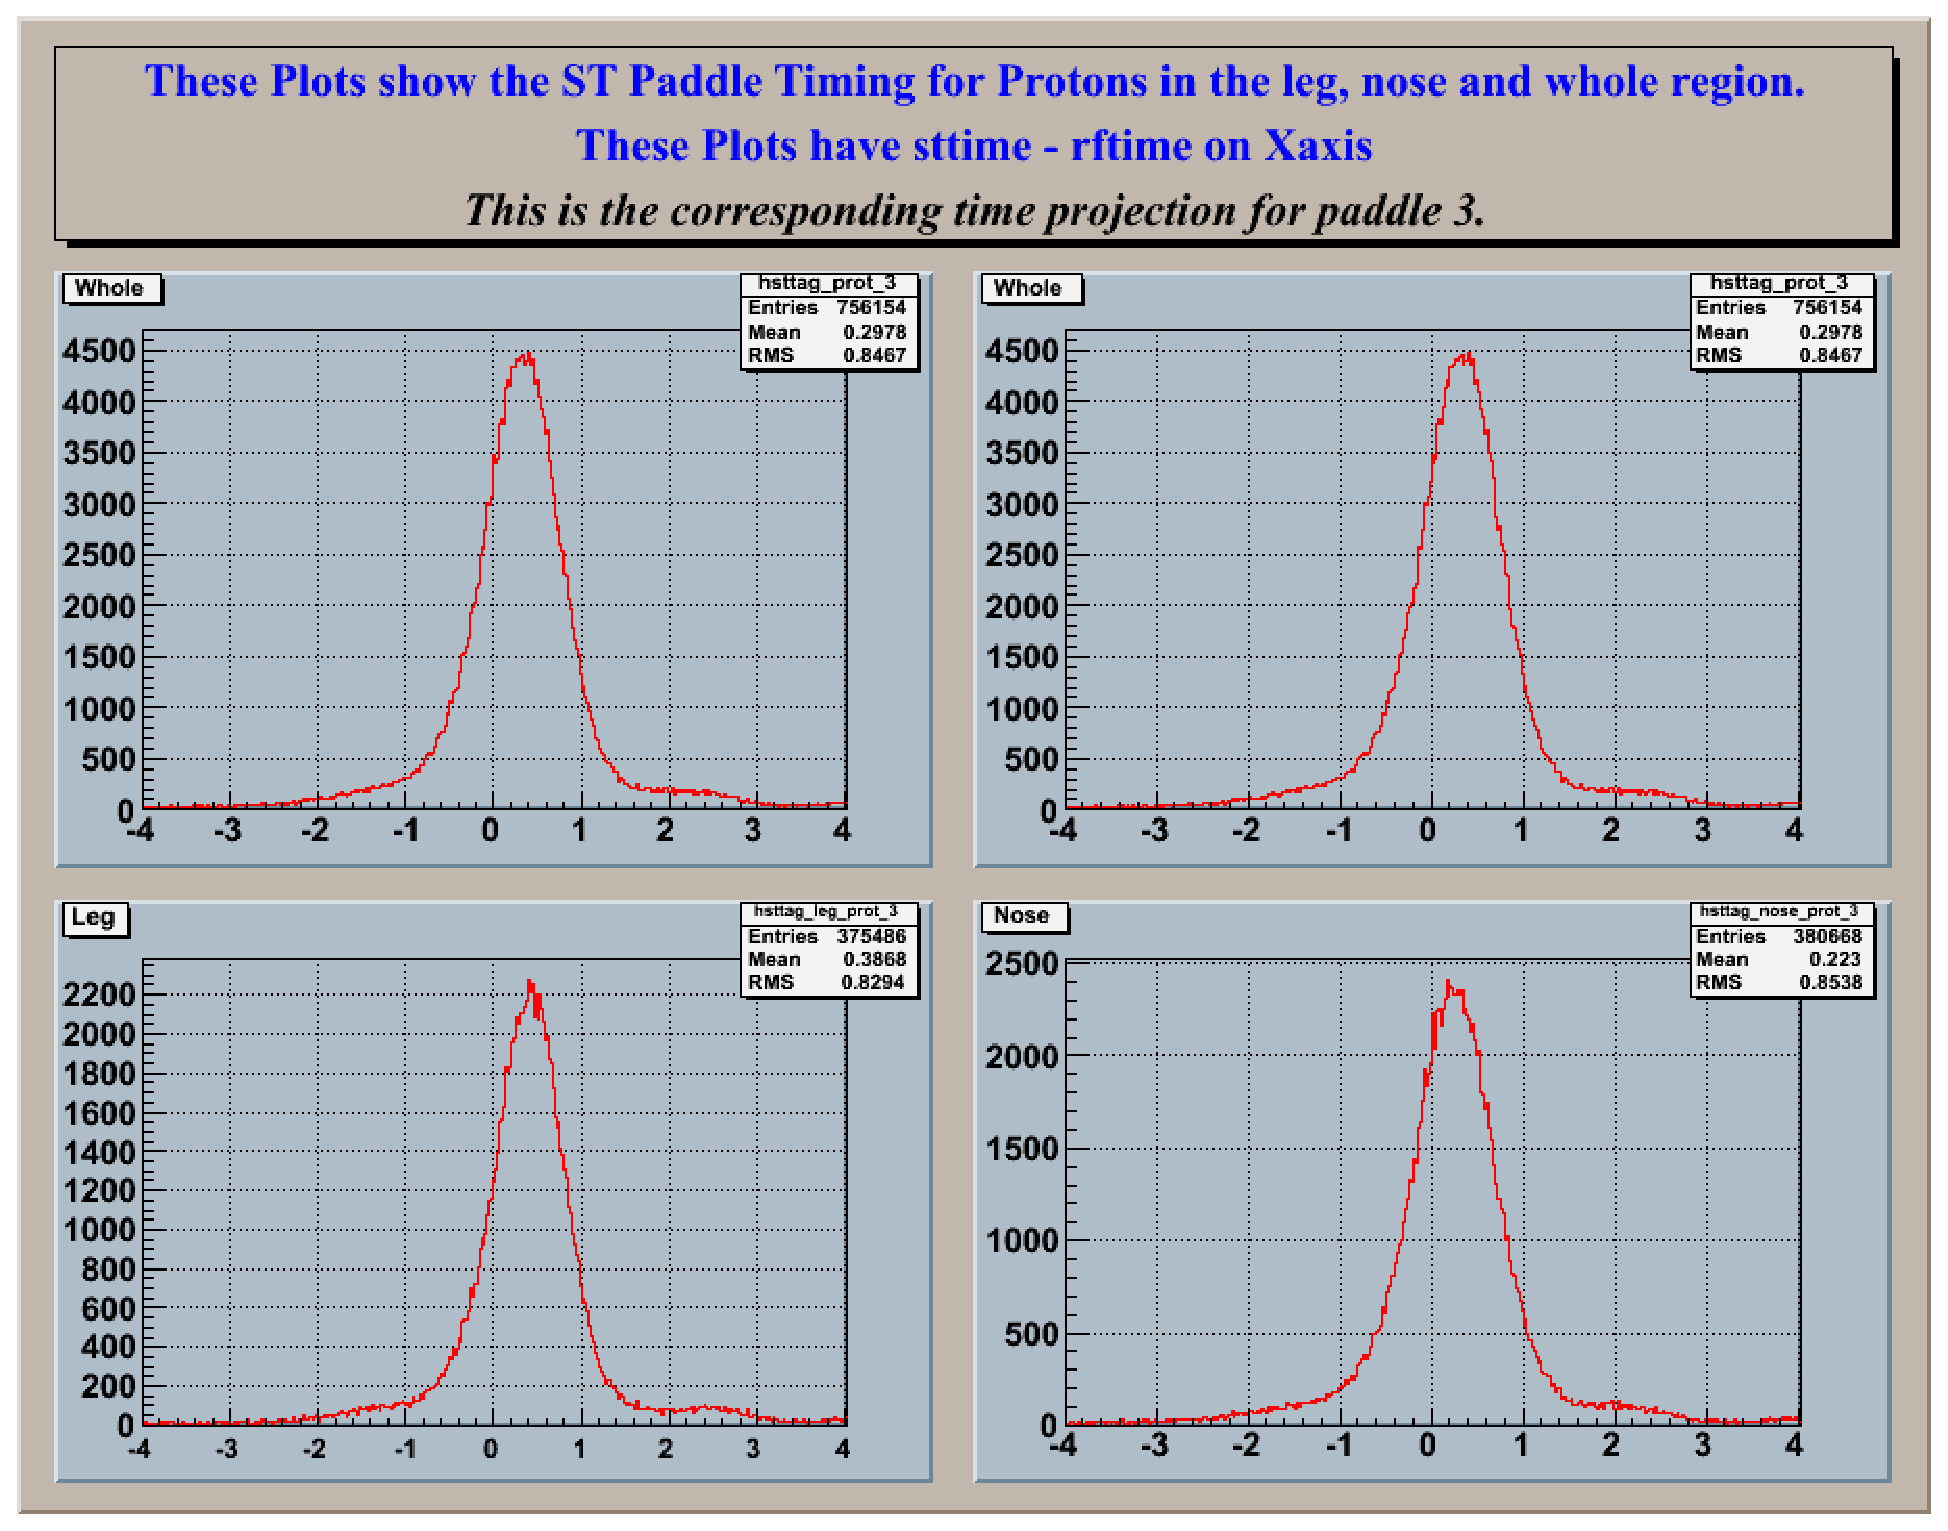
\includegraphics[width=0.65\columnwidth]{figures/calib/st/Hpad3_sttag_prot.eps}
\caption[]{\label{fig:calib.st.timeproton}Same as Fig.~\ref{fig:calib.st.timepion} for protons.}
\end{center}\end{figure}

\begin{figure}[htbp]\begin{center}
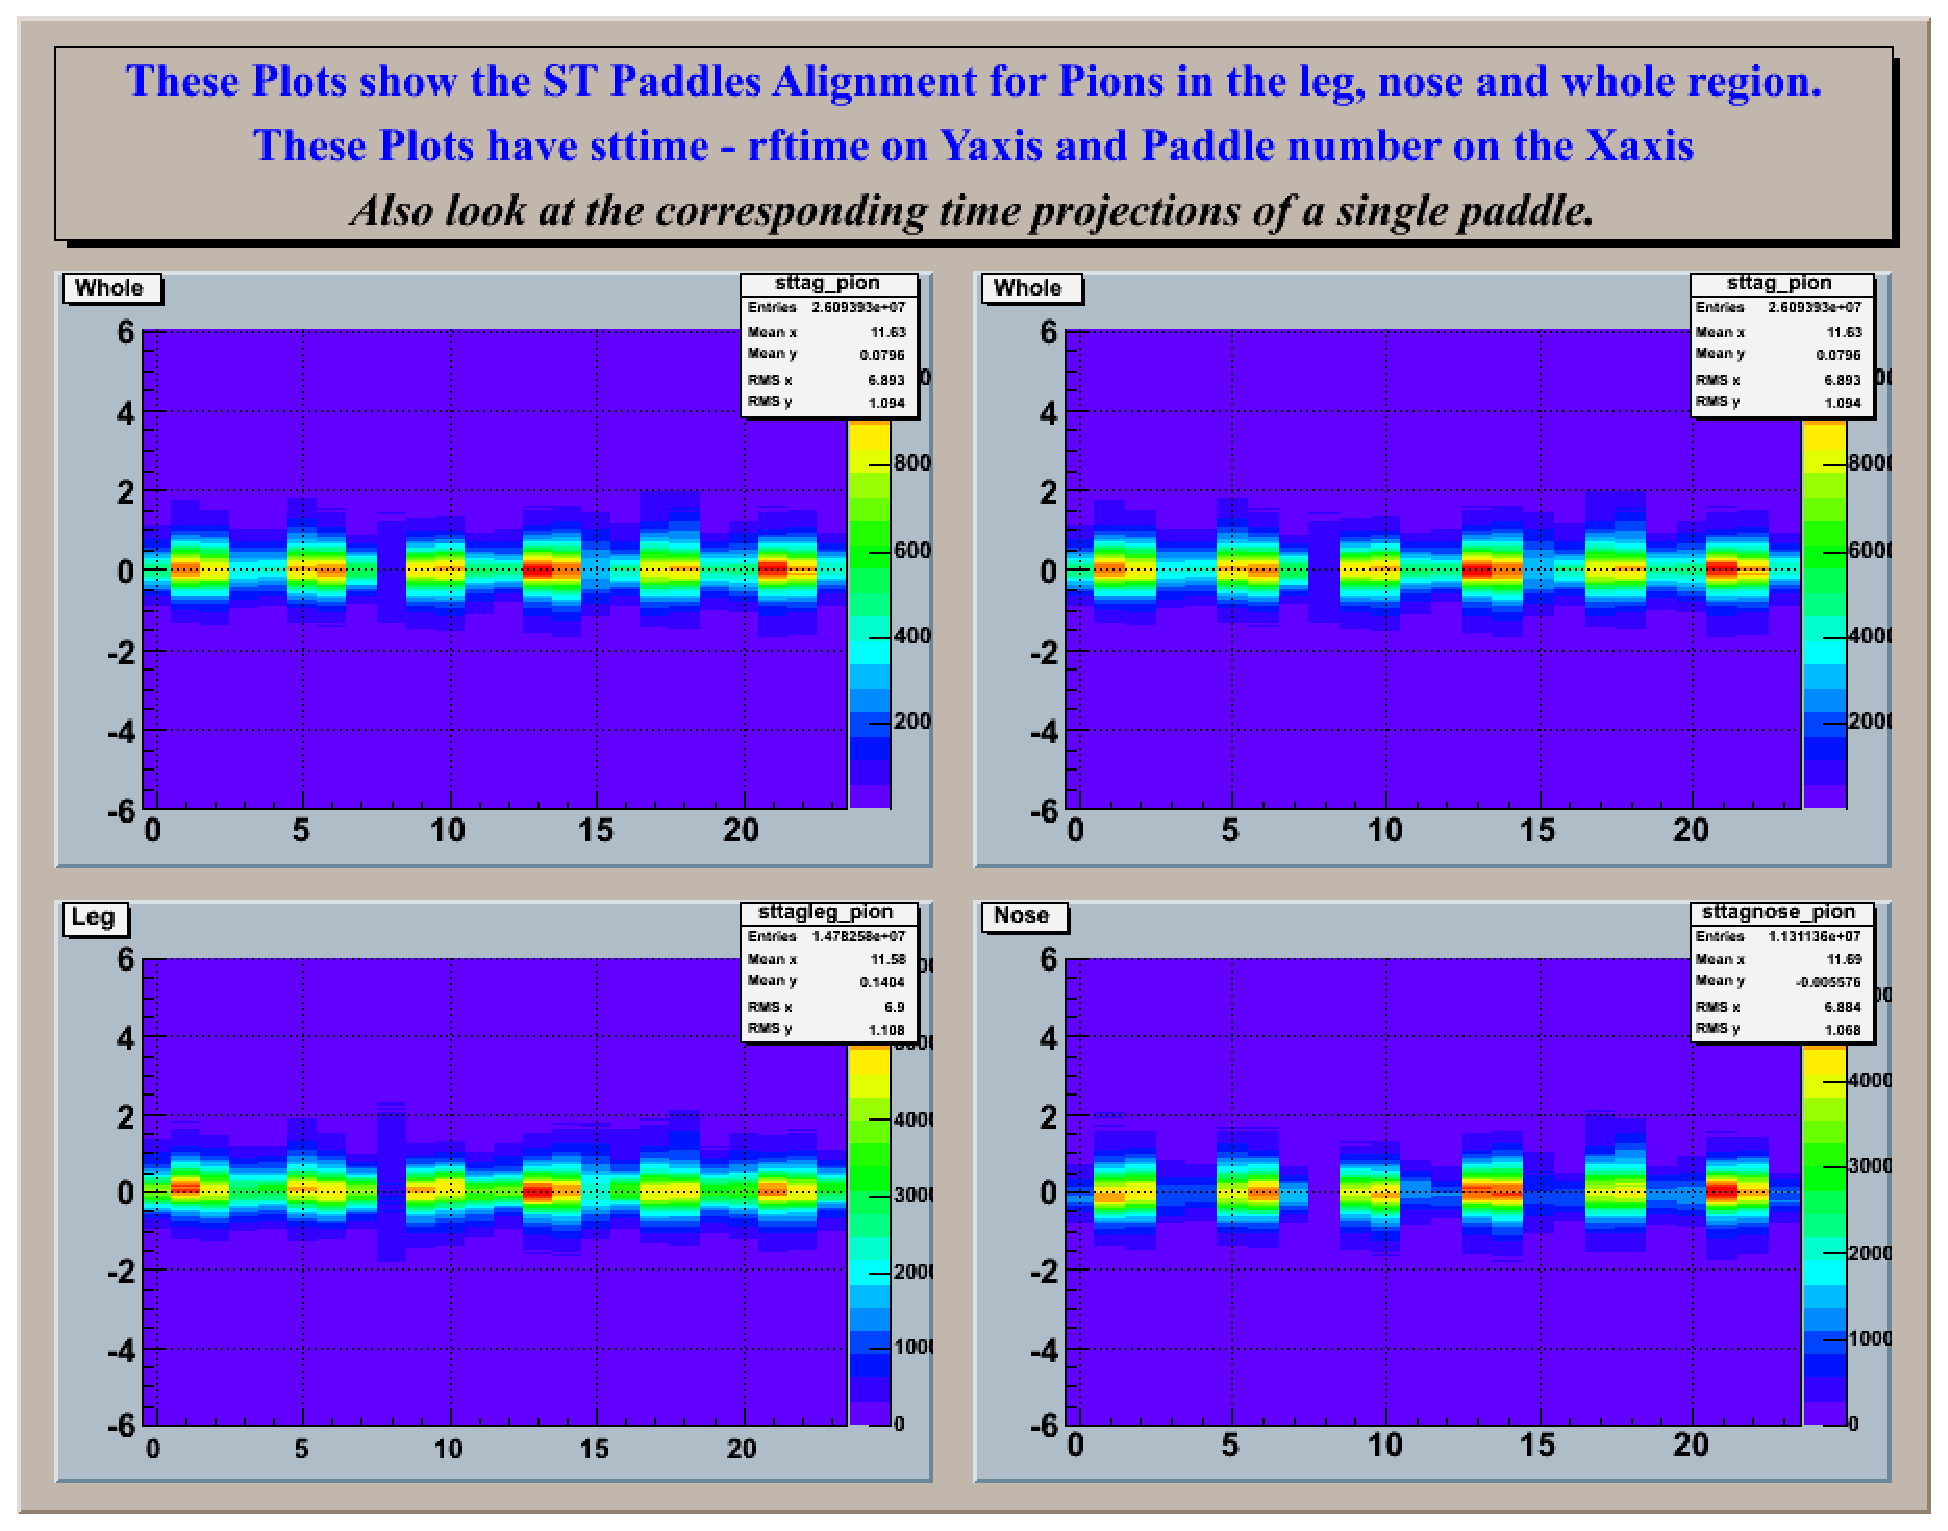
\includegraphics[width=0.6\columnwidth]{figures/calib/st/Hsttag_pion.eps}
\caption[]{\label{fig:calib.st.timepion2d}See caption above.}
\end{center}\end{figure}

\begin{figure}[htbp]\begin{center}
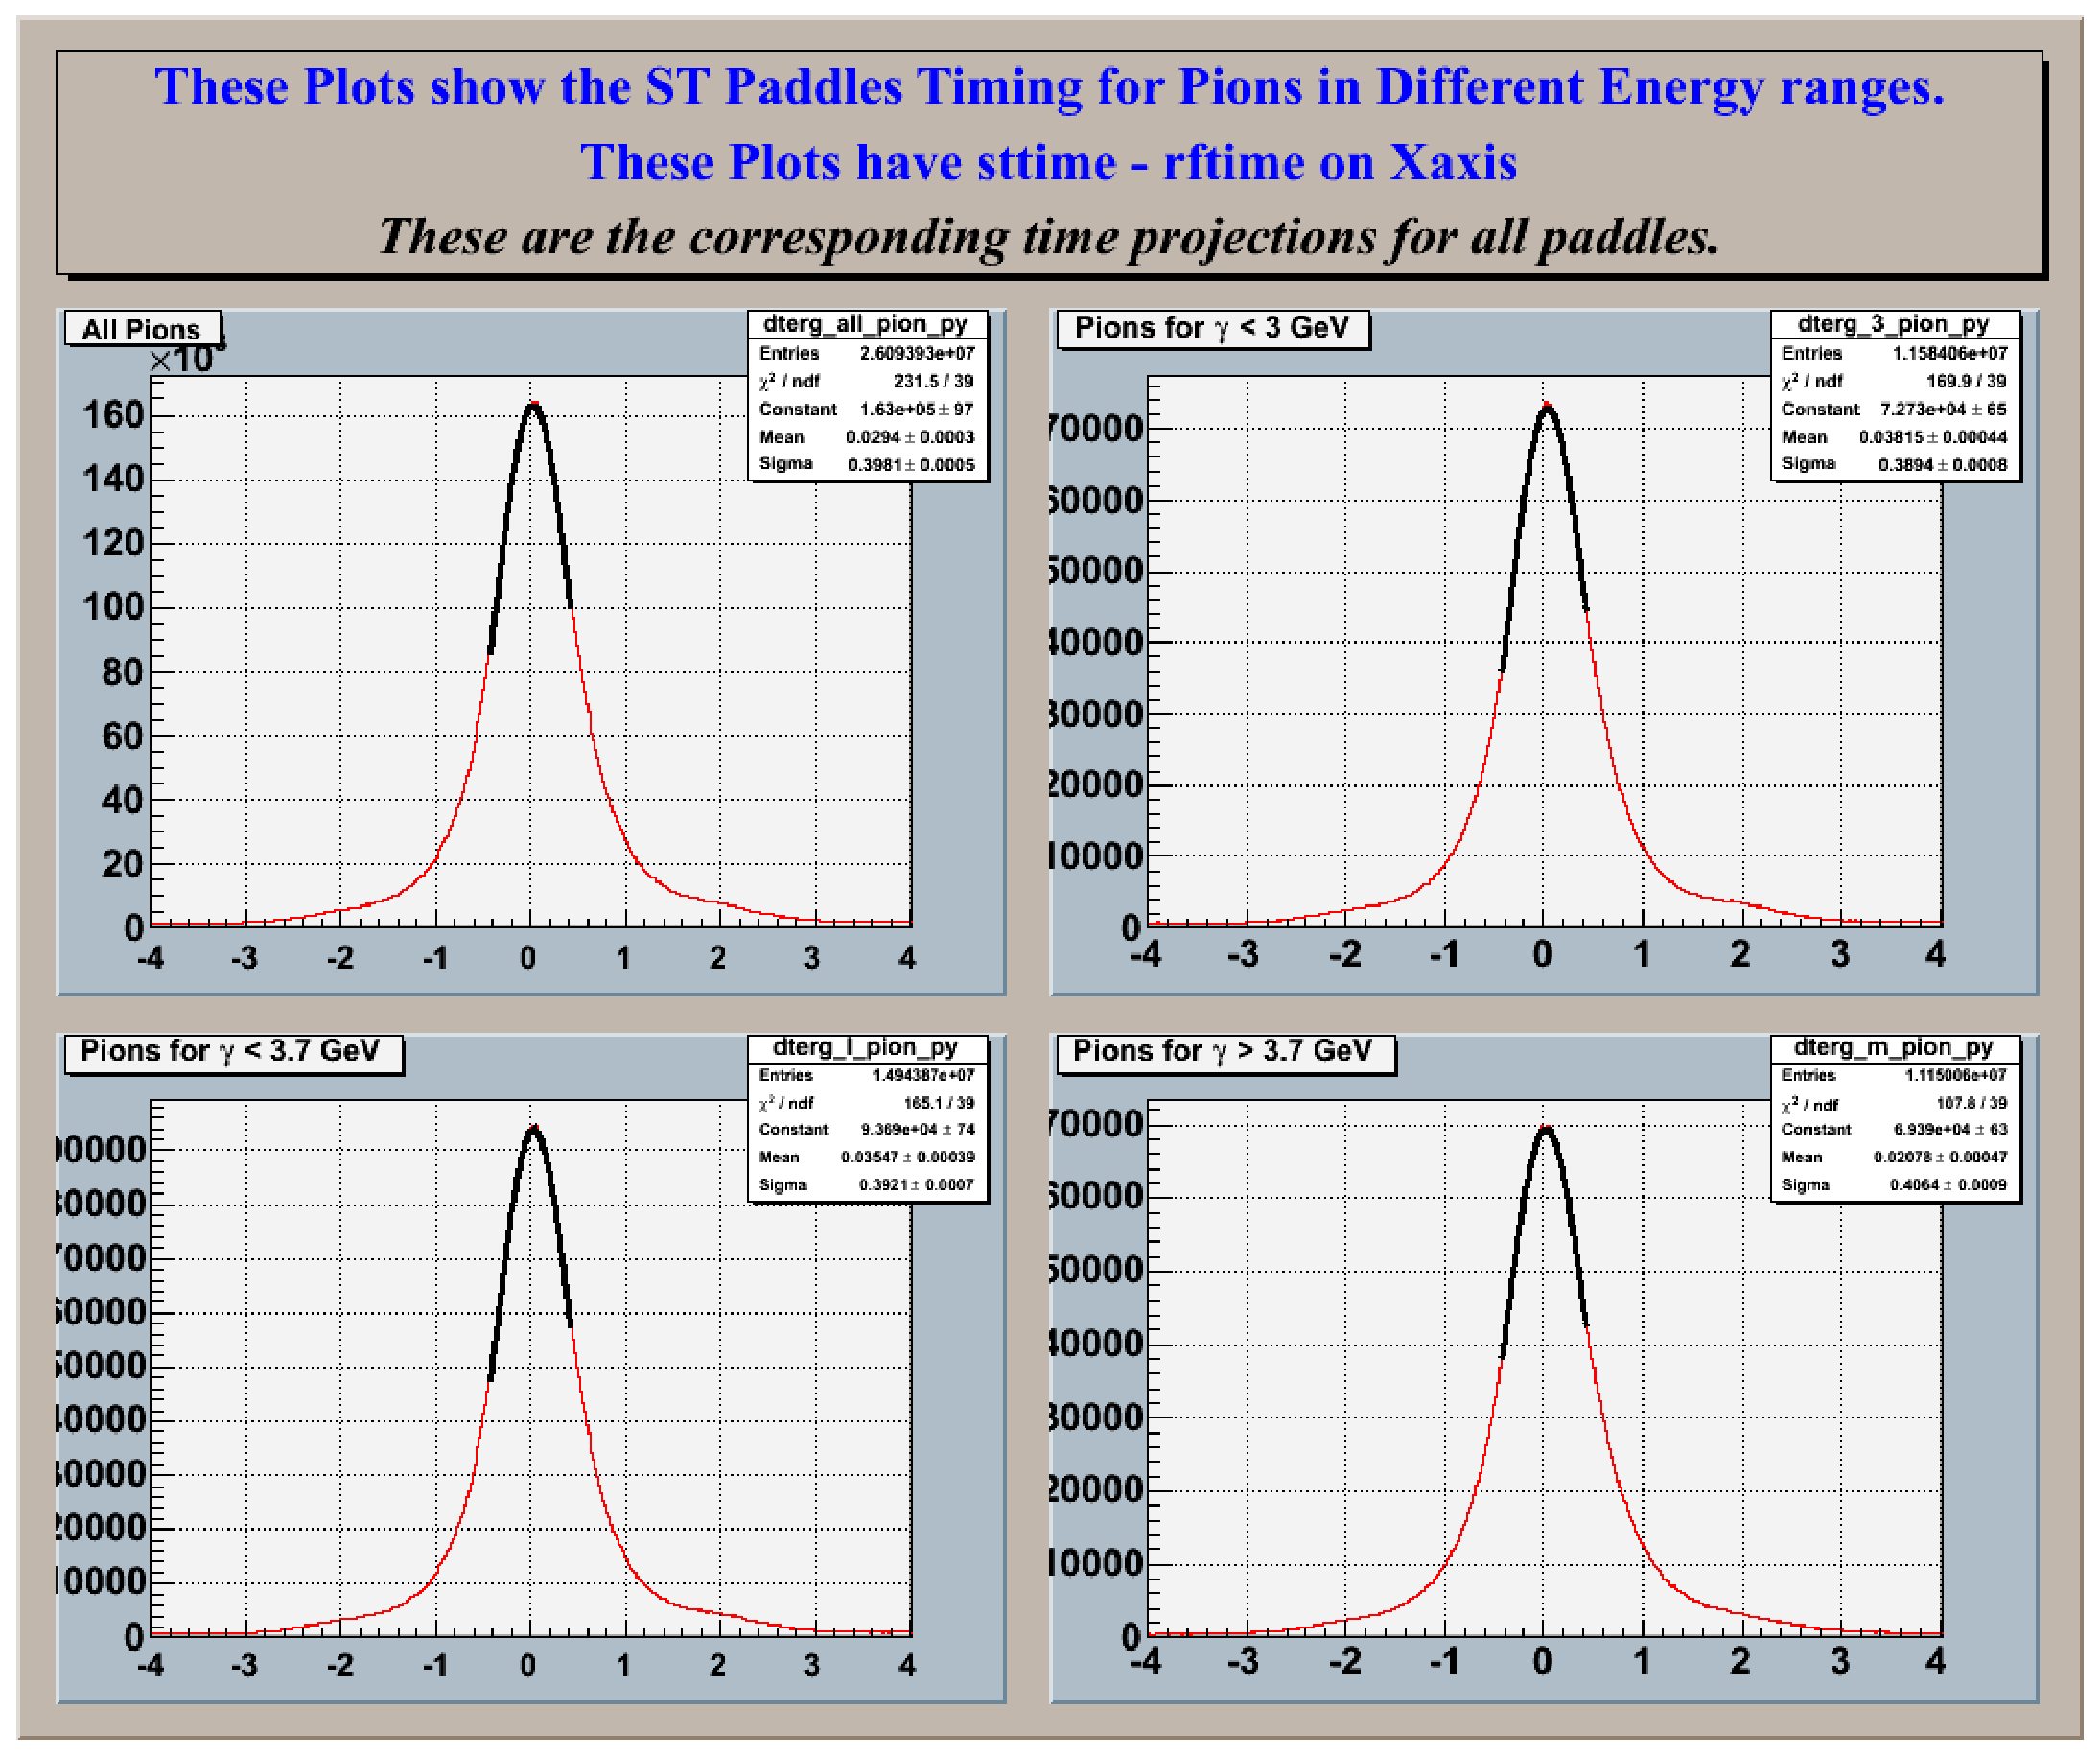
\includegraphics[width=0.6\columnwidth]{figures/calib/st/Sterg_pion.eps}
\caption[]{\label{fig:calib.st.timepion.ebeam}See caption above.}
\end{center}\end{figure}

\begin{figure}[htbp]\begin{center}
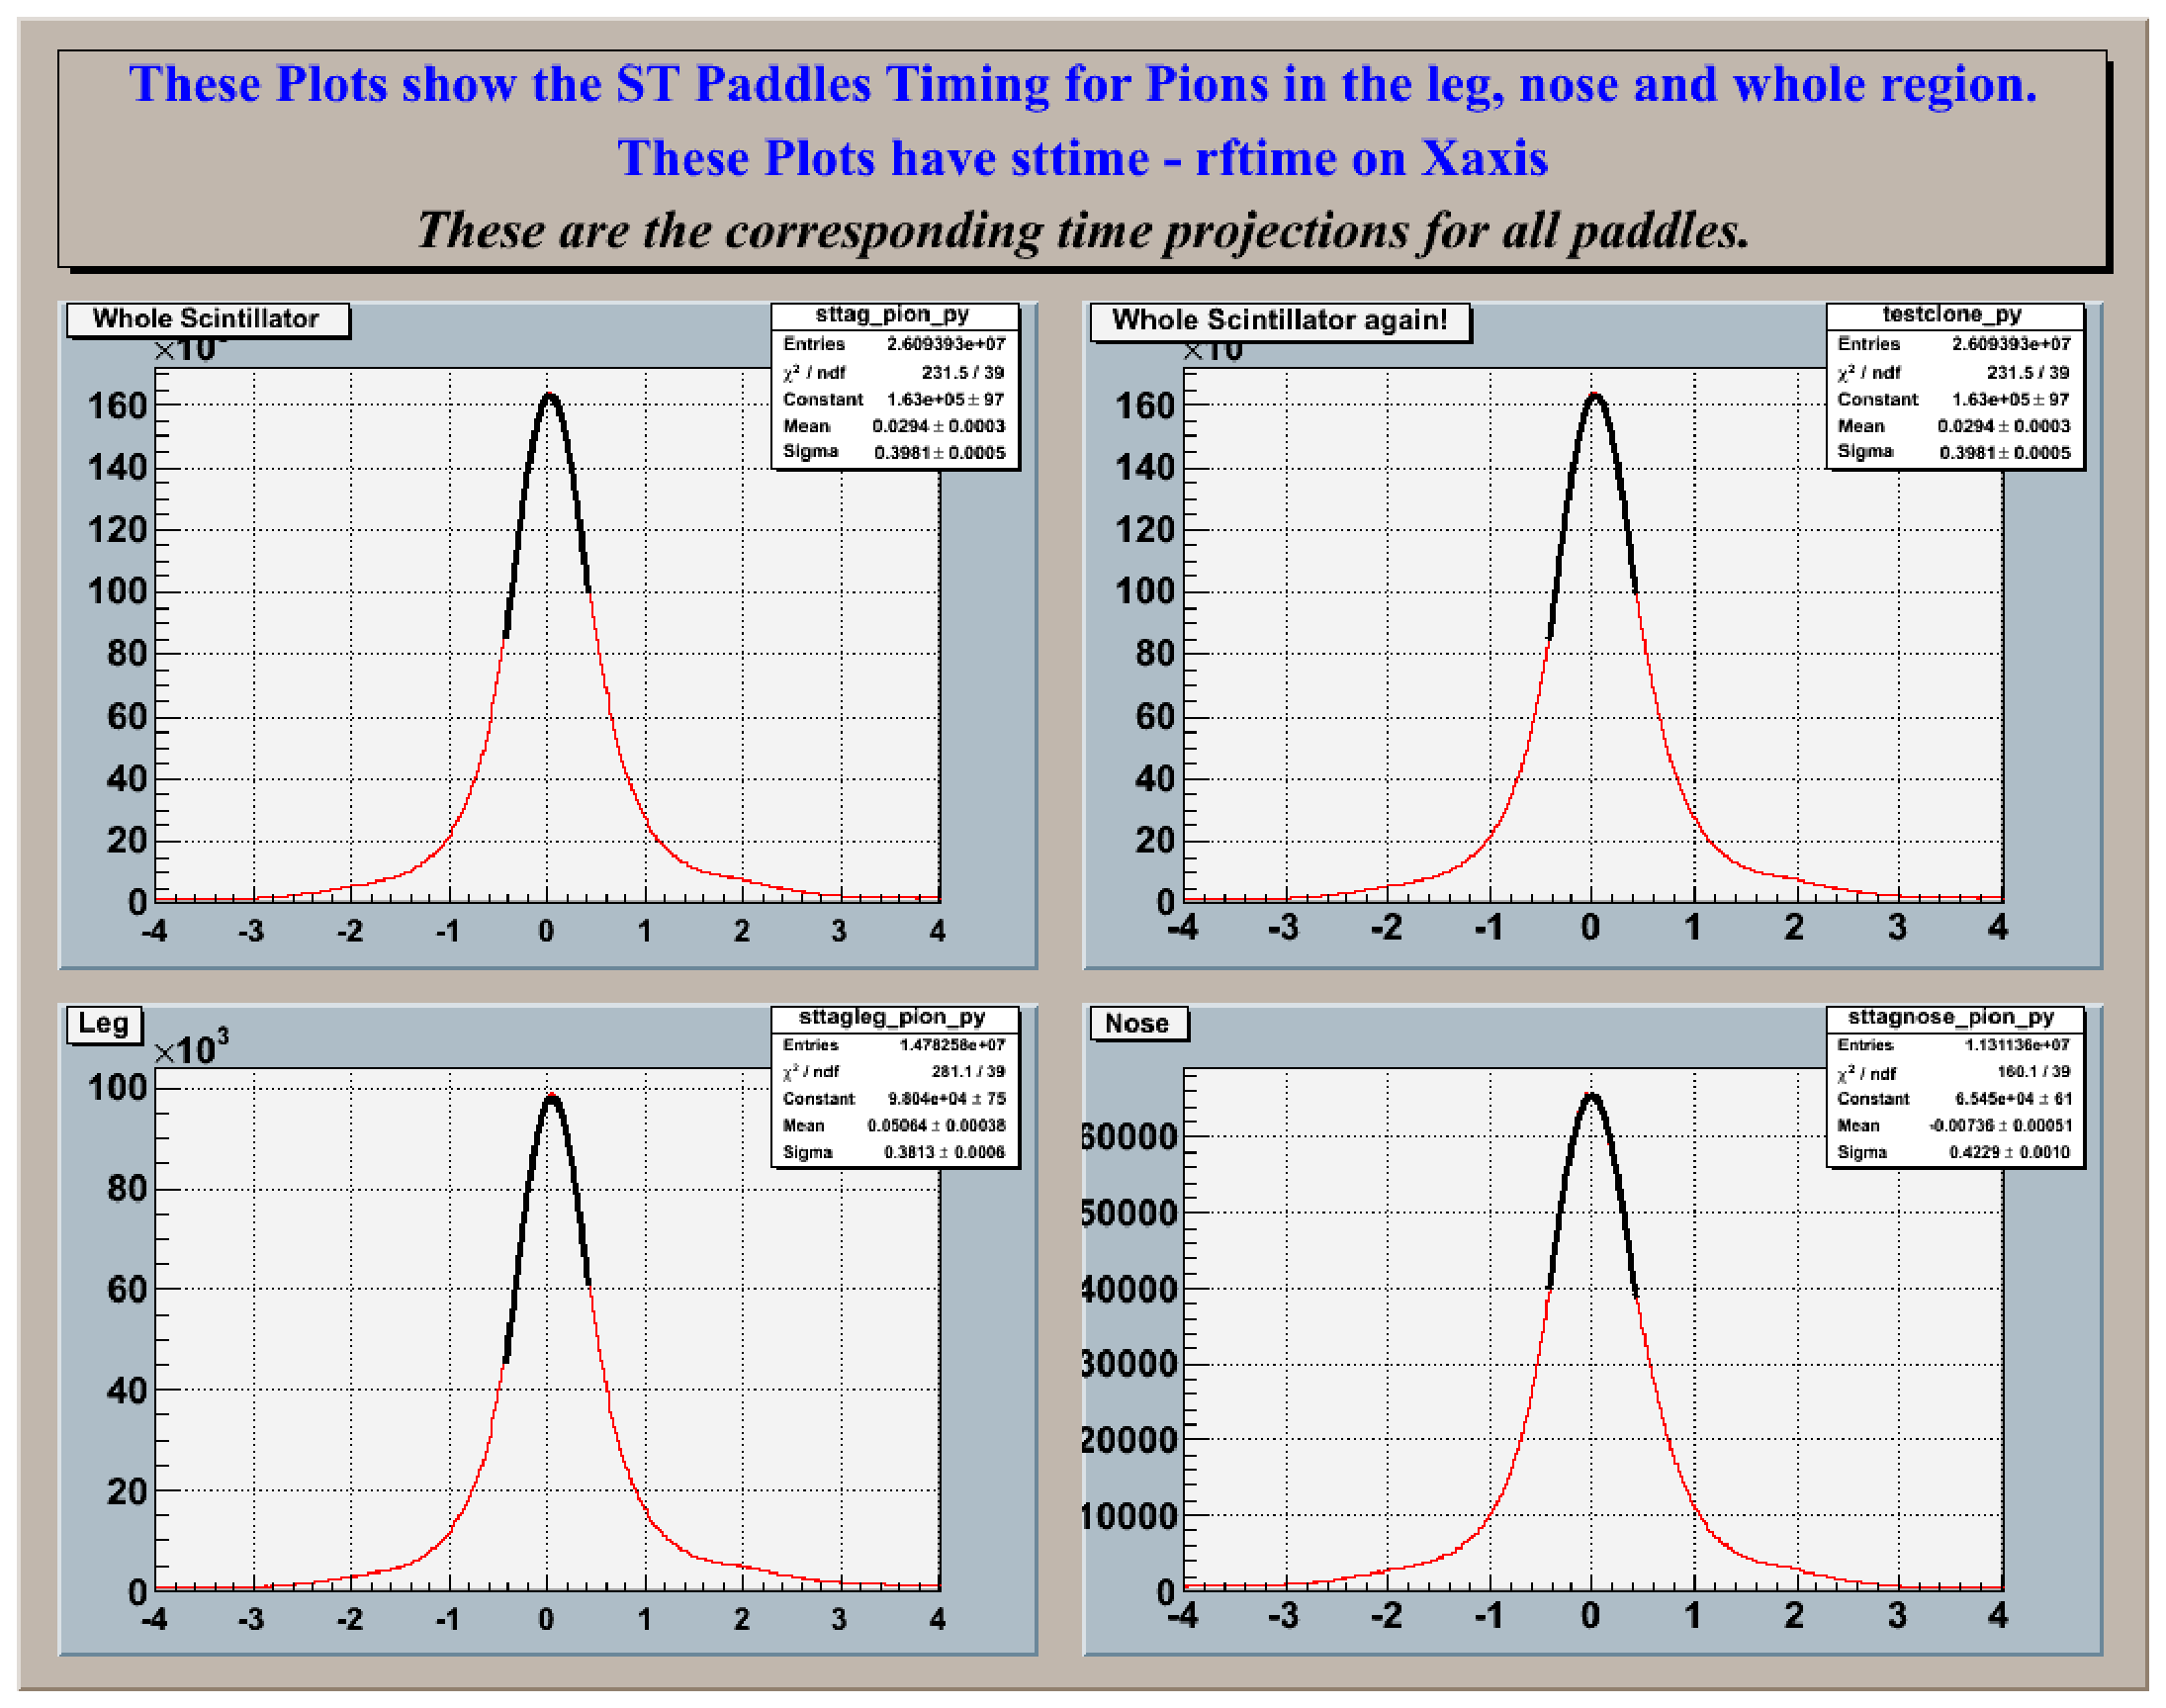
\includegraphics[width=0.6\columnwidth]{figures/calib/st/Timing_pad_3.eps}
\caption[]{\label{fig:calib.st.timepion.region}See caption above.}
\end{center}\end{figure}

\begin{figure}[htbp]\begin{center}
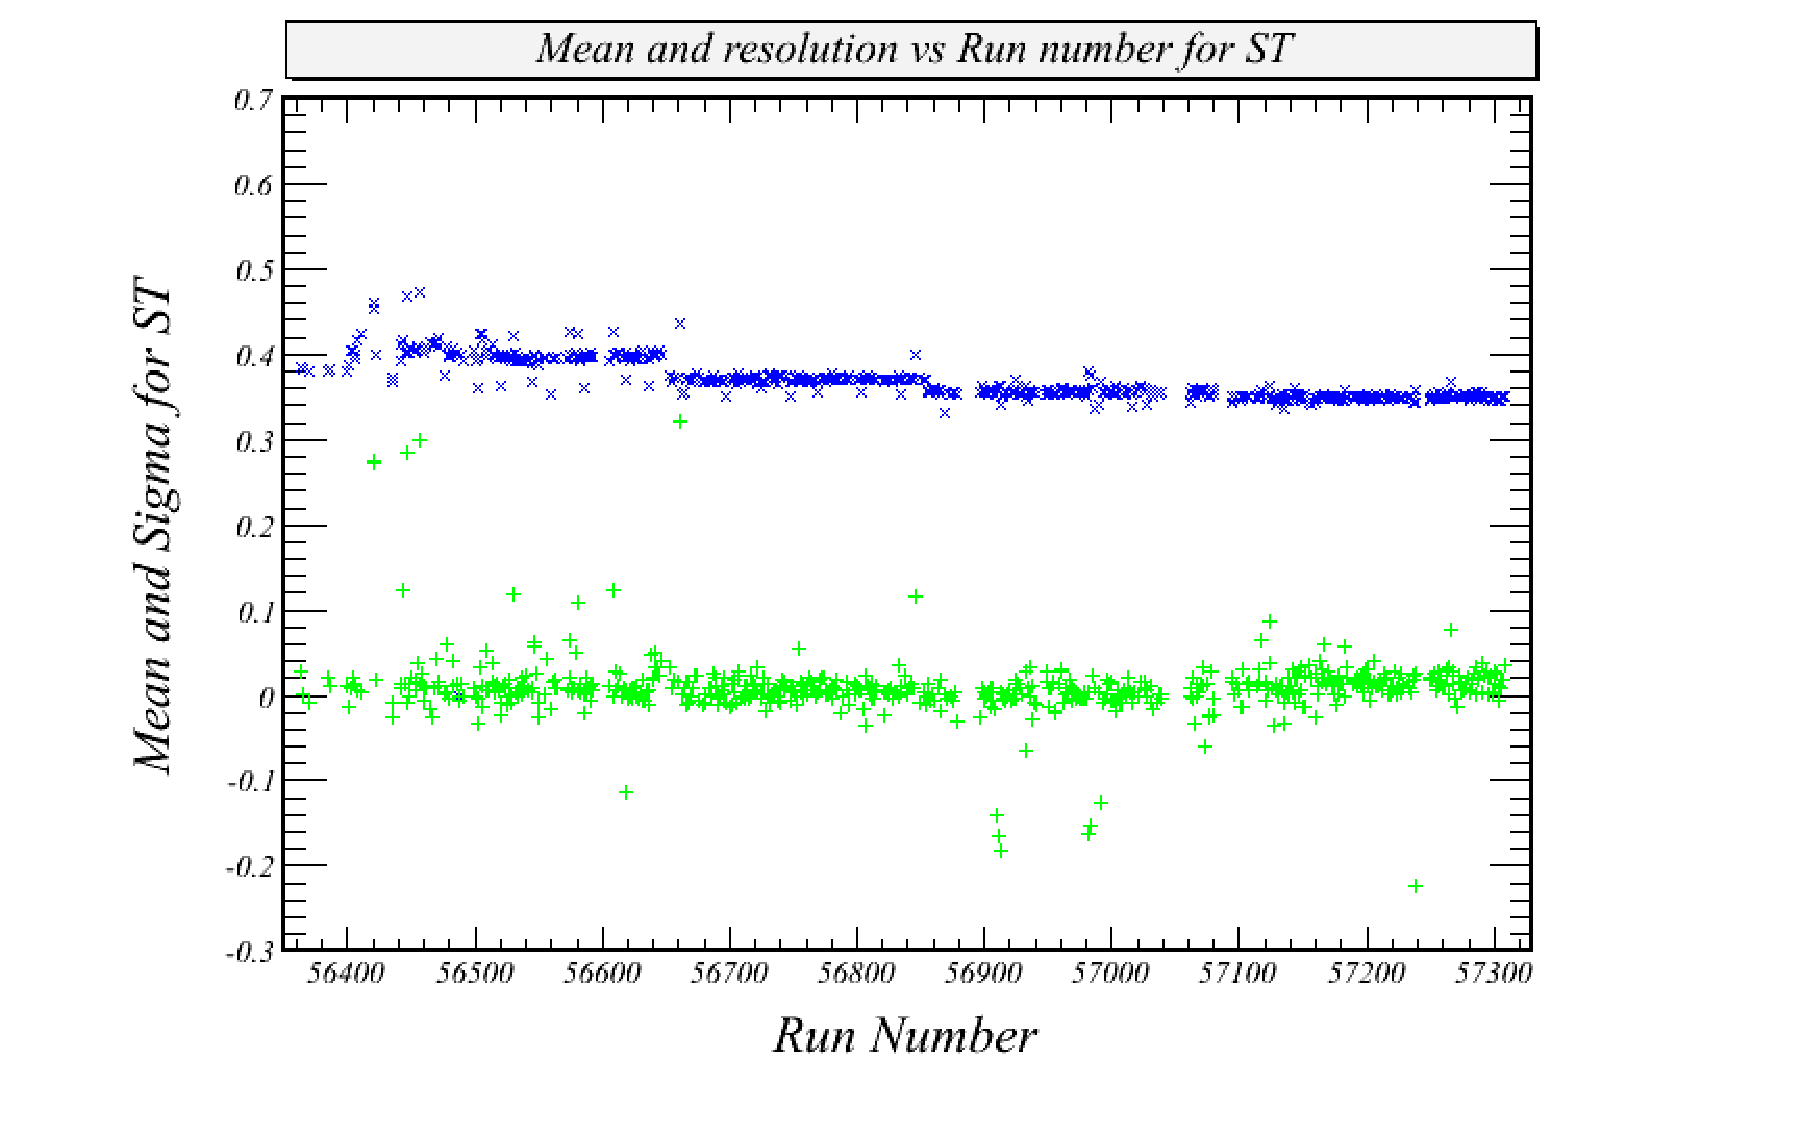
\includegraphics[width=0.65\columnwidth]{figures/calib/st/STmeanandres_v5.eps}
\caption[]{\label{fig:calib.st.runbyrun}Calibrated difference in time between the start counter and RF as a function of run. The mean (green) and 1σ resolution (blue) are shown.}
\end{center}\end{figure}

\FloatBarrier

%%%%%% add ref to 13,14


As a check on the timing resolution of the start counter, we used data containing at least two K$^+$ (this was part of the cascade baryon search) to look at kaons, pion and protons at the same time. The momenta ($p$) of the tracks was given by the drift chamber and tracking algorithm found in the \bank{TBTR} bank, and the energy ($\Epid$) of the particle was set by particle identification. This allowed us to calculate the speed of the particle:
\begin{equation}
    \betapid = \frac{p}{\Epid}.
    \label{eqn:betapid}
\end{equation}
This was used to calculate the vertex time of the particle:
\begin{equation}
    \tvtofpid = \ttof - \frac{\ltof}{c\betapid},
    \label{eqn:tvtofpid}
\end{equation}
where $\ttof$ and $\ltof$ are the time and path length of the track at the \system{TOF} plane as obtained from the \bank{TDPL} bank. This time was converted to a ``photon time'' ($\tpho$) by subtracting the photon propagation time ($\tprop$) from the center of the target:
\begin{equation}
    \tphotofpid = \tvtofpid - \tprop,
    \label{eqn:tphotofpid}
\end{equation}
where
\begin{equation}
    \tprop = \frac{1}{c} \left( \ztgt - \zv \right),
\end{equation}
where $\ztgt$ is the center of the target's z-position ($-90$~cm in the \system{CLAS} coordinate system), and $\zv$ is the z-coordinate of the track's vertex position -- in this case, the intersection of the two kaons where the covariance matrices of the estimated momenta are taken into account through the standard \prog{MVRT} vertexing algorithm. This photon time, $\tphotofpid$, was compared to the \system{RF}-corrected tagger times ($\ttgrf$, shown in Figs.~\ref{fig:dvertex_time_pid_st} and \ref{fig:dvertex_time_st}) of each hit in the photon tagger as obtained from the \bank{TAGR} bank. The resulting data indicates a timing resolution of 310~ns for protons, 400~ns for pions, and 430~ns for kaons.

\begin{figure}[htbp]\begin{center}
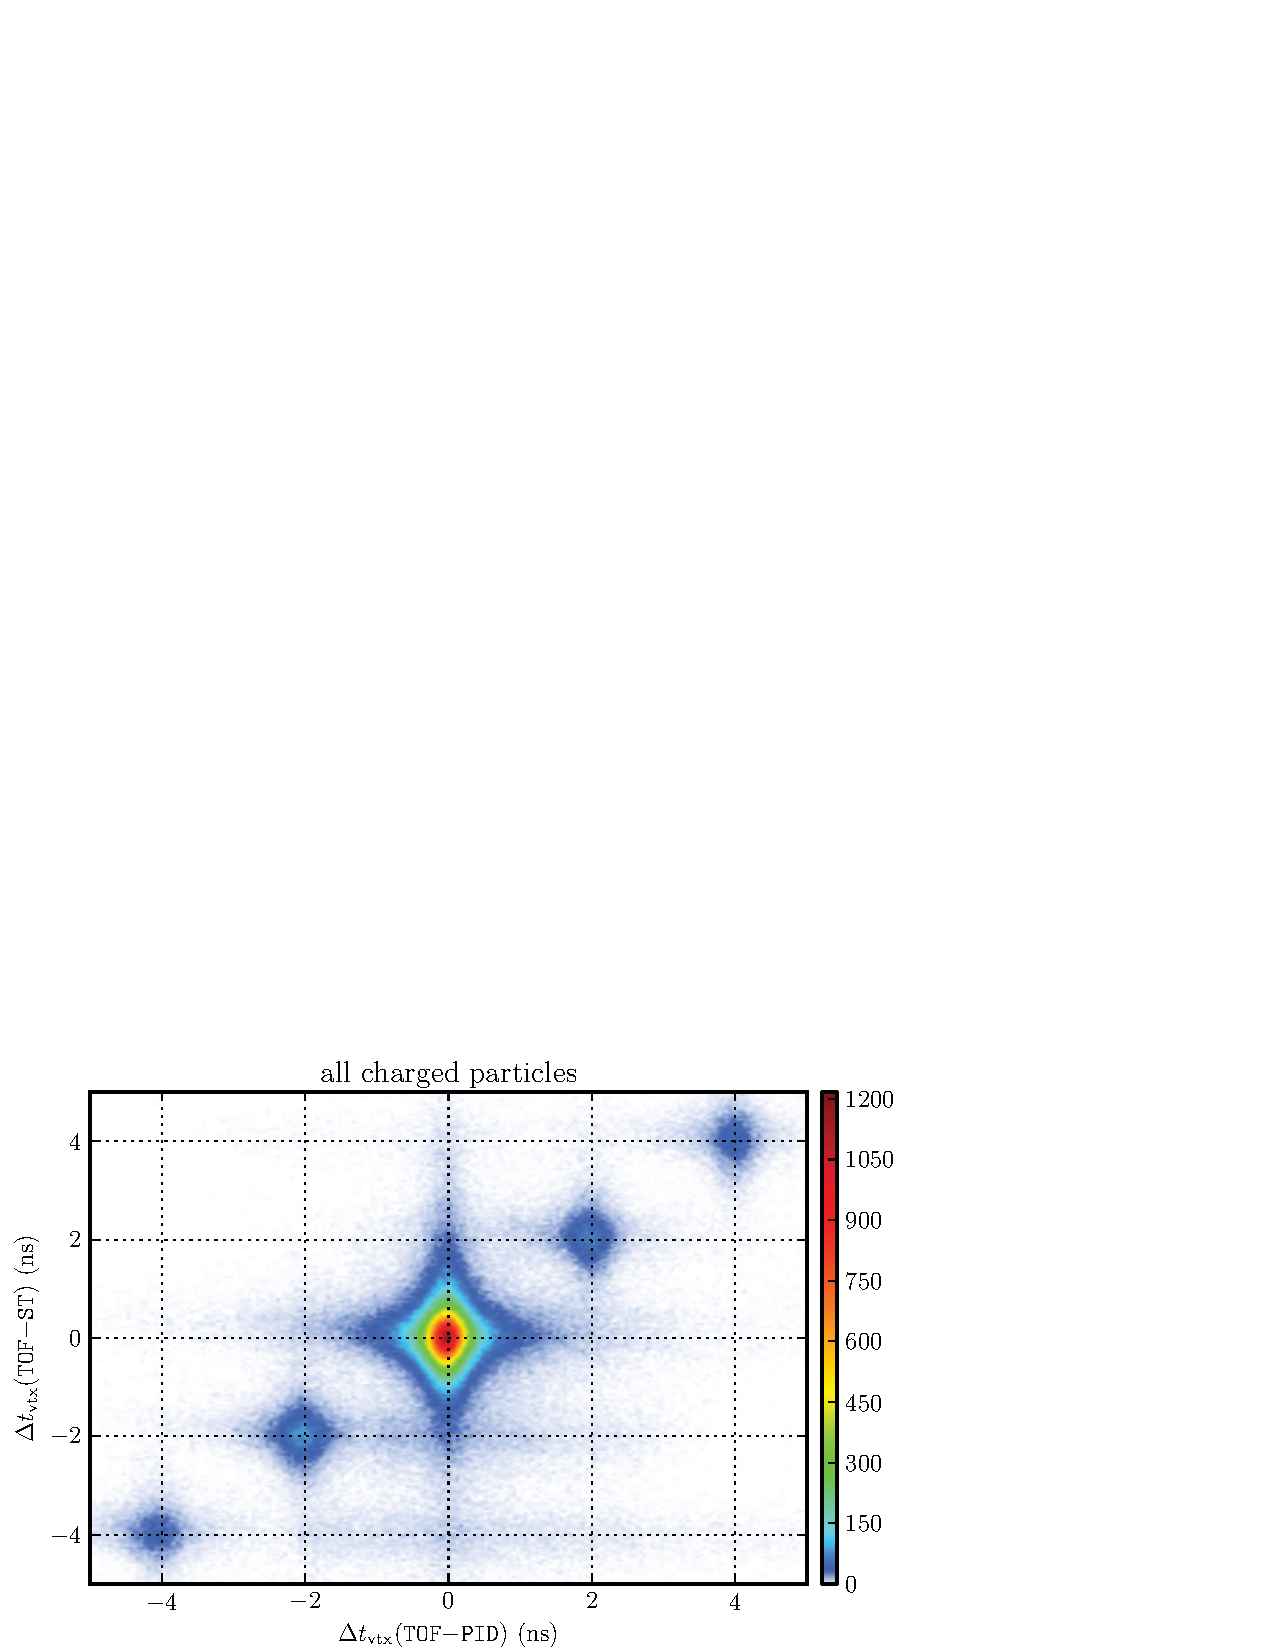
\includegraphics[width=0.5\columnwidth]{figures/calib/st/dvertex_time_pid_st.pdf}
\caption[vertex timing, \abbr{TOF-ST} vs.\ \abbr{TOF-PID}]{\label{fig:dvertex_time_pid_st}Difference in vertex times for each track for the two calculations made above. Represents 1.5\% of the total statistics.}
\end{center}\end{figure}

\begin{figure}[htbp]\begin{center}
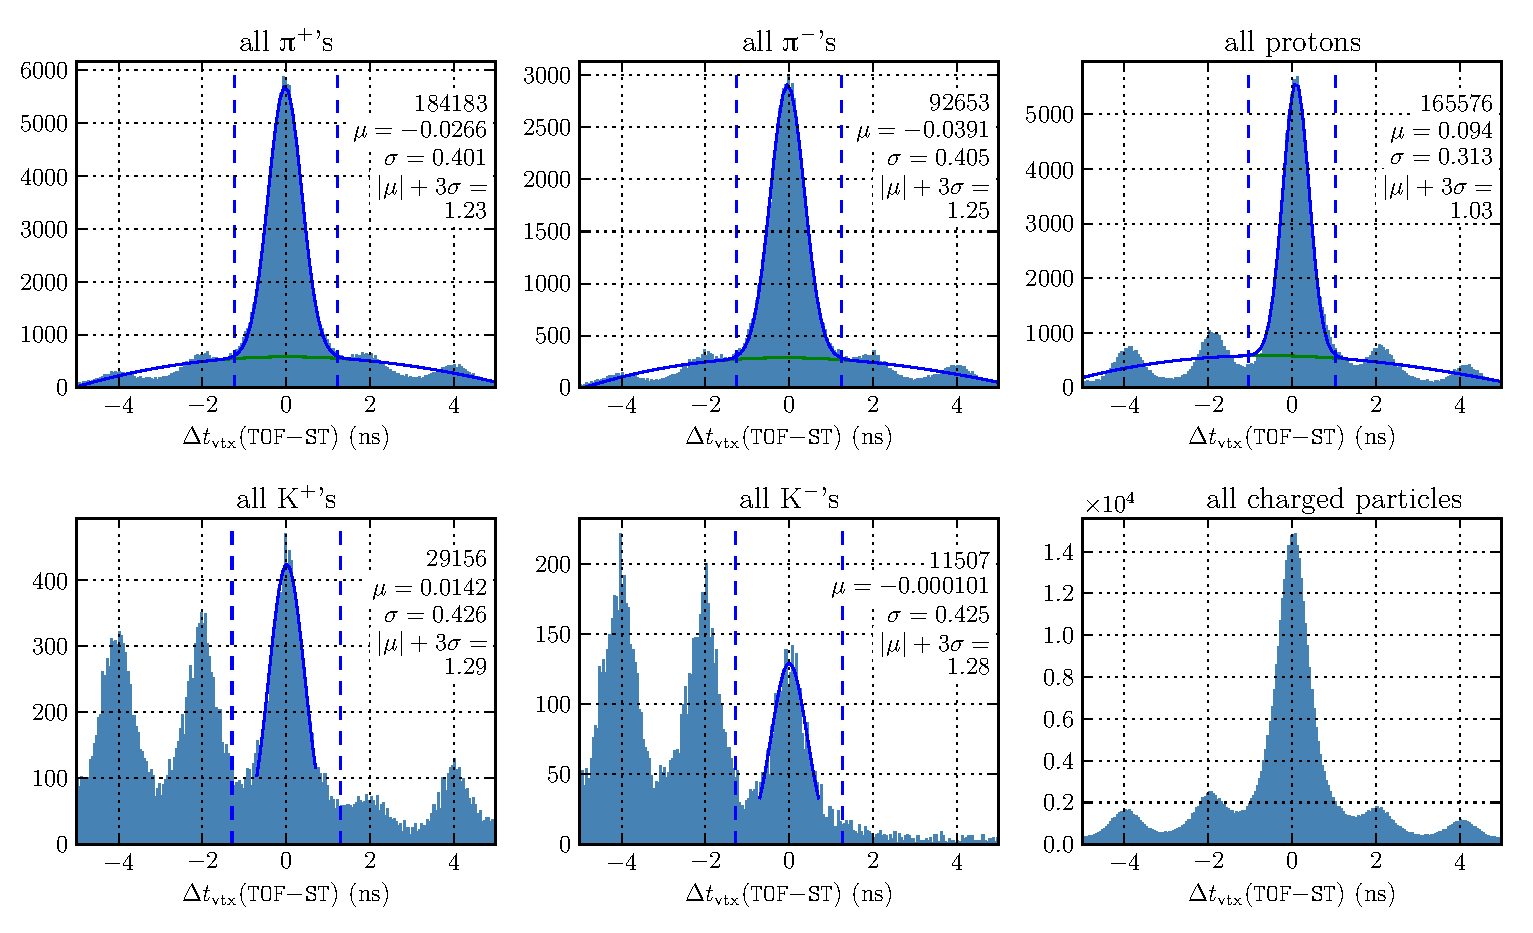
\includegraphics[width=0.9\columnwidth]{figures/calib/st/dvertex_time_st.eps}
\caption[vertex timing, \abbr{TOF-ST}]{\label{fig:dvertex_time_st}Difference in vertex time between that of the photon and of the tracks based on start counter and time-of-flight times. Represents 1.5\% of the total statistics.}
\end{center}\end{figure}


\subsubsection{\label{sec:calib.st.eff}Start Counter Efficiency}

The efficiency of the start counter was calculated by examining the number of tracks with a ST hit after track reconstruction. The ST fired $91.6\%$ of the time, this was calculated from run 57000 since it is a good run and included in production data. This percentage was calculated for the start counter as a whole. Any analysis that uses associated start counter hits with identified tracks must take this efficiency into account. Note, however, that this effect is very small ($< 1 \%$) for many-particle final states where only a single start counter is required.

\FloatBarrier

\subsection{\label{sec:calib.dc}Drift Chamber Calibration and Resolution}

Tracking in the Drift Chamber of a \abbr{CLAS} Sector is performed using the six superlayers of the \abbr{DC}. A good measure of the the quality of tracking are the \abbr{DC} residuals for each superlayer. After a track is identified using the hit elements in the \abbr{DC} superlayer, It's \abbr{DC} residual is calculated using the TBLA bank as follows:

\begin{verbatim}
fabs(TBLA->tbla[i].fitdoca) - fabs(TBLA->tbla[i].calcdoca)
\end{verbatim}

\begin{v2}The Drift Chamber alignment was done by correcting the mean of the residuals and the results are shown in Fig.~\ref{fig:dc.align}.\end{v2}  The values of the \abbr{DC} residuals in the \abbr{CLAS} data are empirically found to be a good fit to a convolution of 2 Gaussians - a narrow Gaussian and a broad Gaussian. During \abbr{DC} calibrations efforts were made to minimize this residual to have maximum reconstruction efficiency. The mean and width of the residuals as a function of superlayer and run number are shown in Figs.~\ref{fig:calib.dc.residuals.mean} and \ref{fig:calib.dc.residuals.wid} respectively.

\begin{figure}\begin{center}
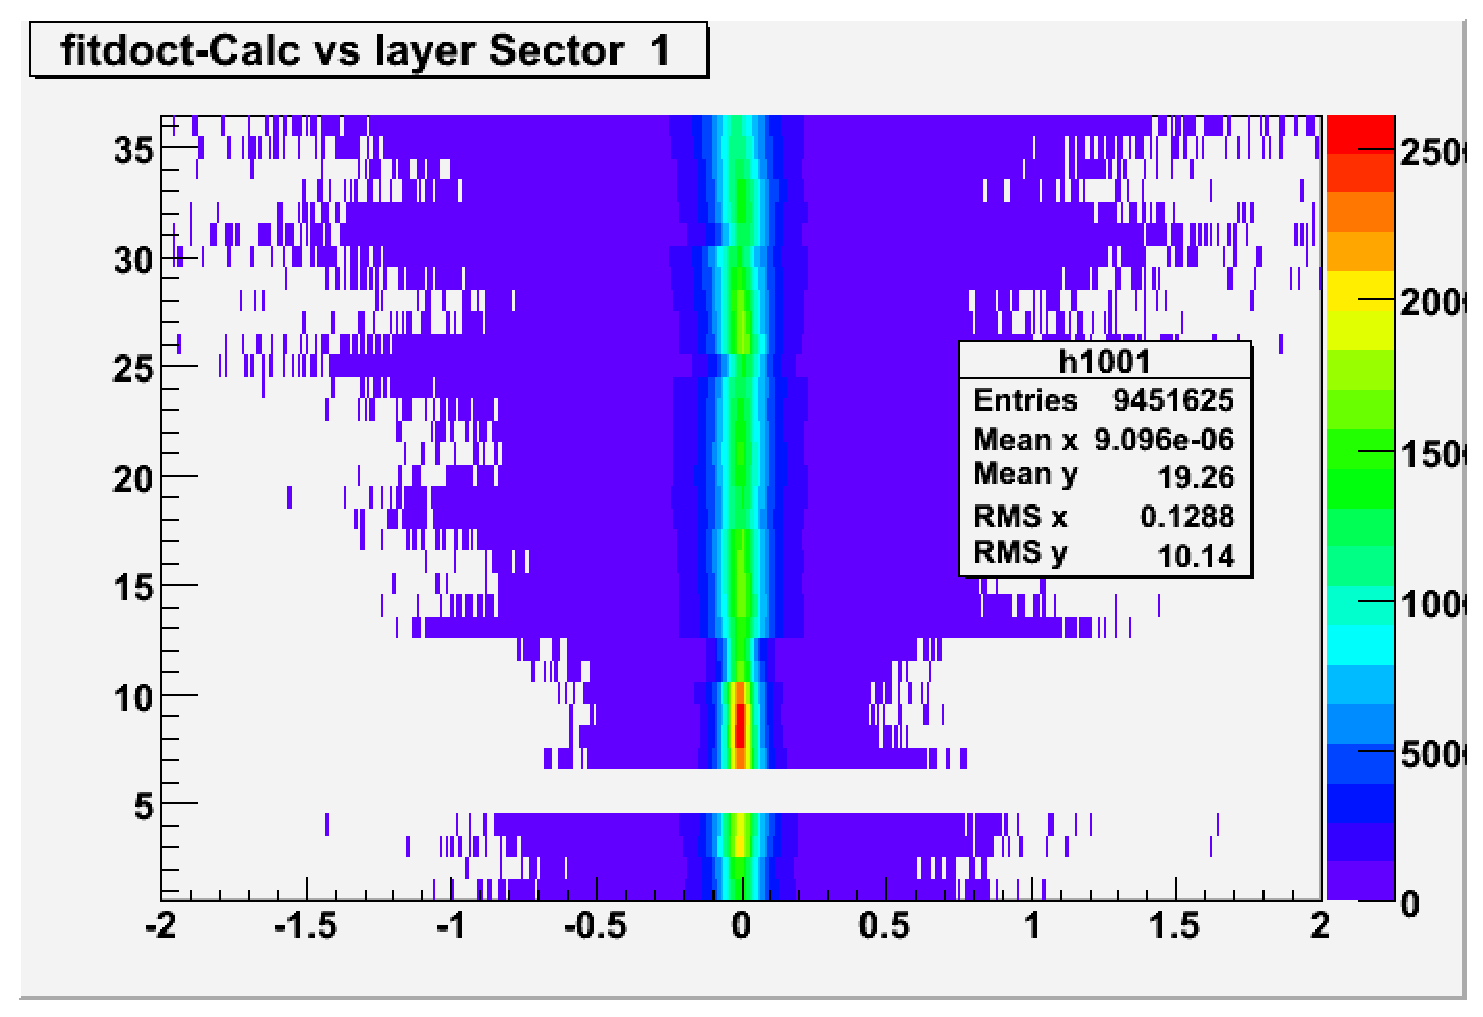
\includegraphics[width=0.6\textwidth]{figures/calib/dc/dc_align1.eps}
\caption[DC Alignment]{\label{fig:dc.align}Alignment of the Drift Chambers in sector 1. All other sectors show very similar results.}
\end{center}\end{figure}

\begin{figure}\begin{center}
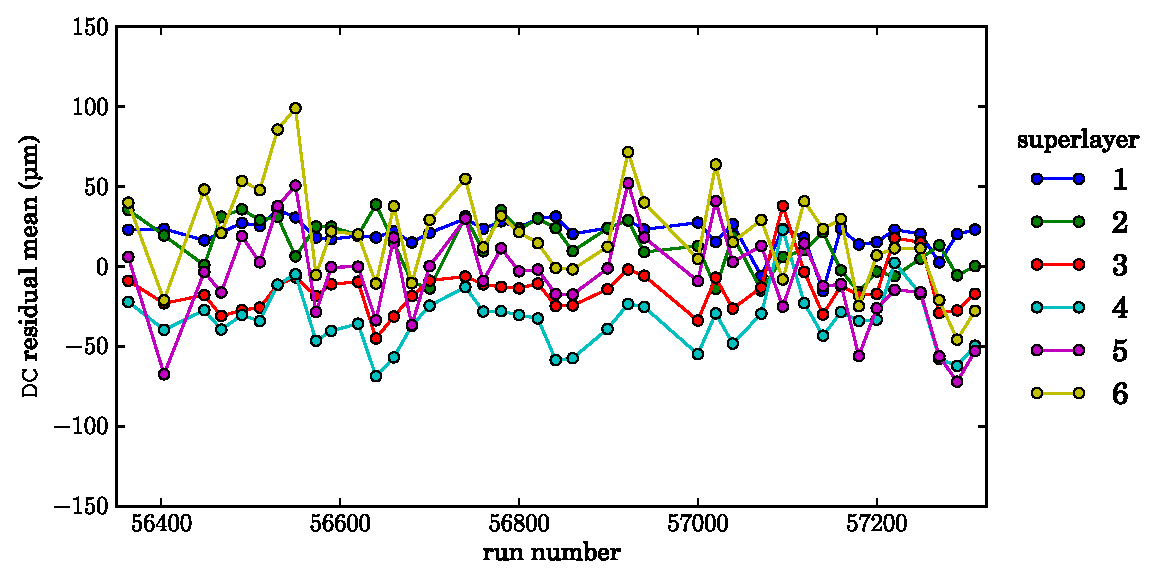
\includegraphics[width=0.6\textwidth]{figures/calib/dc/dc_resid_mean.eps}
\caption[DC Residuals (Mean)]{\label{fig:calib.dc.residuals.mean}Mean of residuals for the drift chambers by superlayer and by run.}
\end{center}\end{figure}

\begin{figure}\begin{center}
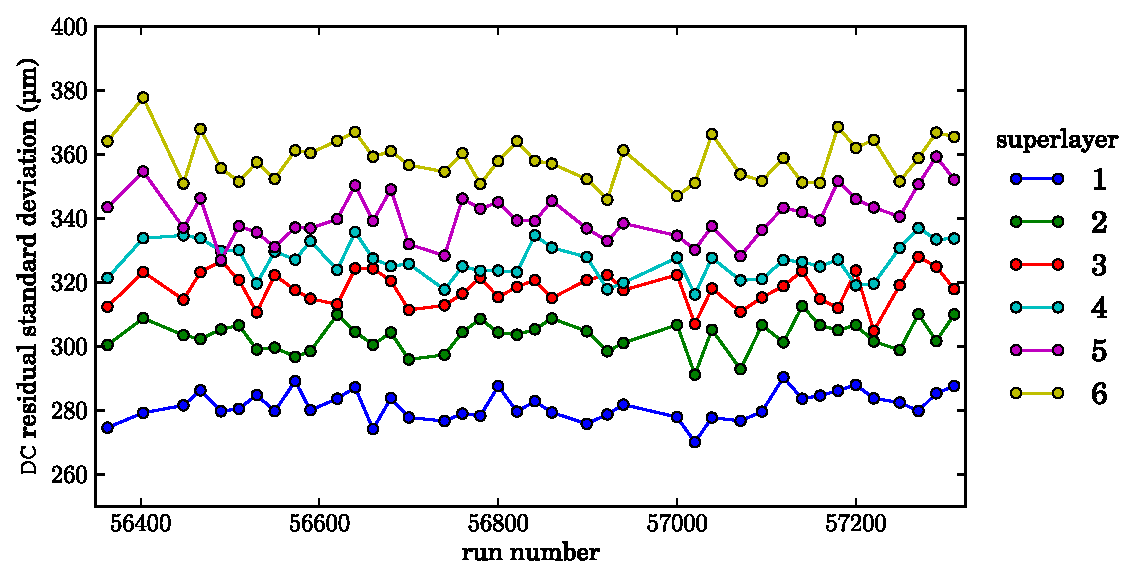
\includegraphics[width=0.6\textwidth]{figures/calib/dc/dc_resid_sigma.eps}
\caption[DC Residuals (Width)]{\label{fig:calib.dc.residuals.wid}Gaussian width of residuals for the drift chambers by superlayer and by run.}
\end{center}\end{figure}

\subsubsection{\label{sec:calib.dc.eff}Drift Chamber Wire Efficiency}

To generate the wire map for \desg{g12}, the utility \prog{pdu}, available in \abbr{SVN}, was used. Maurizio Ungaro made the wire-maps for \desg{g12} with the root files [\verb+A01+ and \verb+A02+] for each run. These output files are at \url{/home/mukesh/work/pdu_hbook} at \abbr{Jlab}. Root files needed are at \url{/home/mukesh/work/pdu_root}. The values were added to the \desg{g12} database. The results of the wire map are plotted in for each sector and can be found here:
\begin{verbatim}
http://www.jlab.org/~ungaro/maureepage/proj/dceff/dc_periods/g12.html
\end{verbatim}
\begin{v2}An example plot from this site is shown in Fig.~\ref{fig:calib.dc.eff}. The DC wire efficiencies were computed for each wire using the whole data set, using the CLAS utility \prog{pdu}. An example of this is shown in the beginning of DC calibration section. Simulation data all use the \prog{gpp} to apply this efficiency map. Comparison of the real data and MC data depends on the topology and model.\end{v2}

\begin{figure}\begin{center}
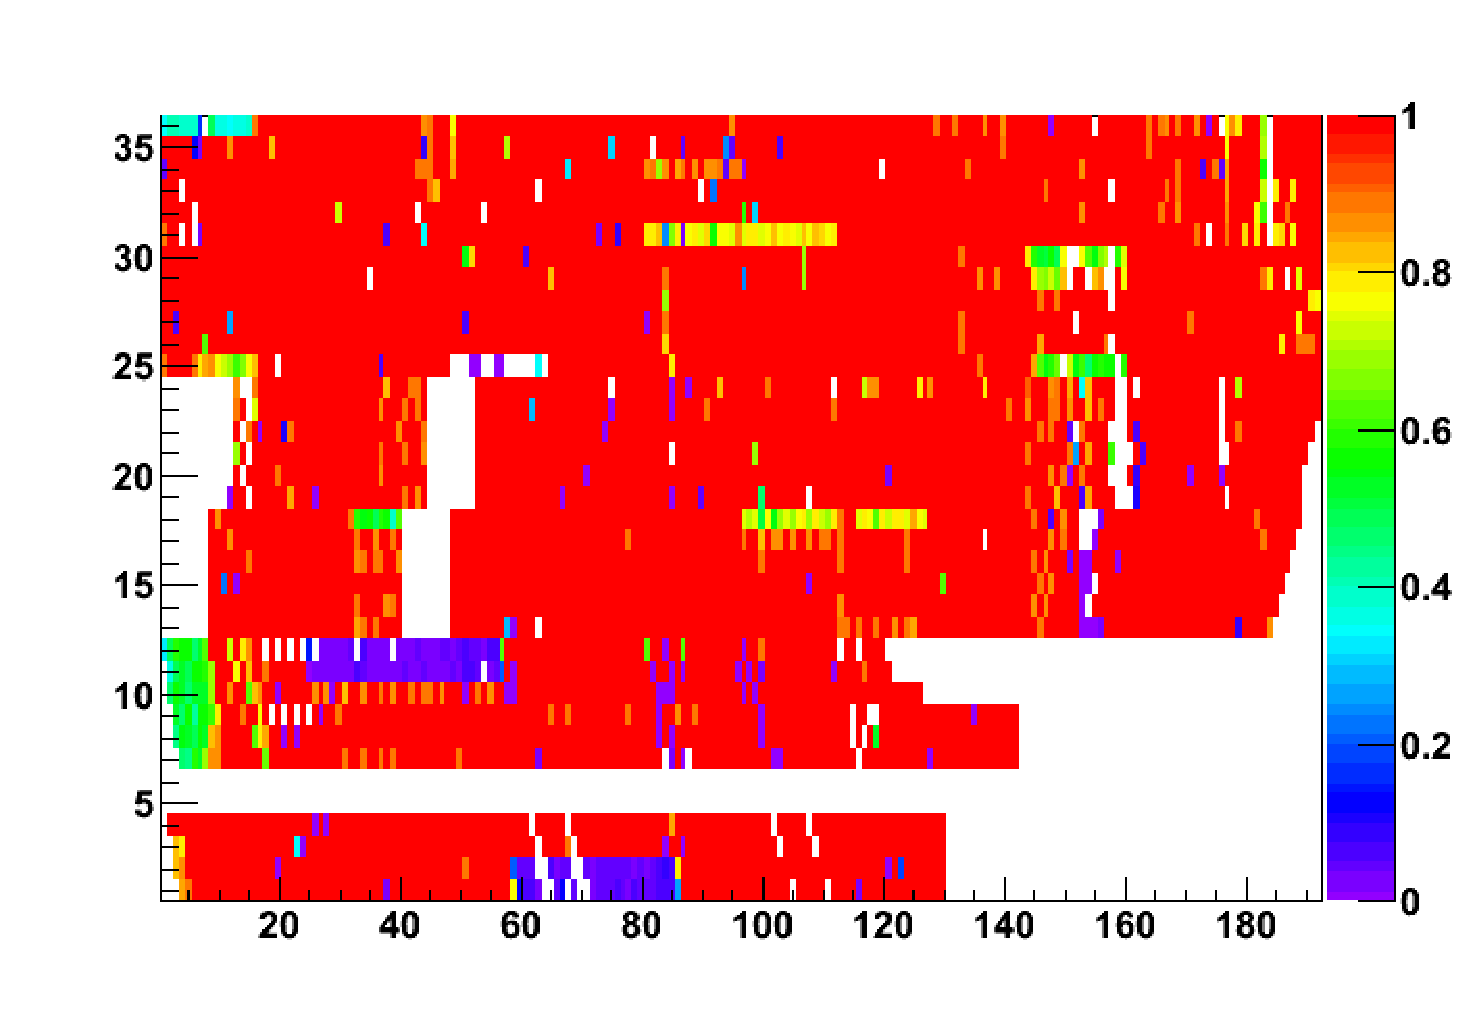
\includegraphics[width=0.6\textwidth]{figures/calib/dc/Occupancy_g12_s1.eps}
\caption[DC Efficiency Map Sector 1]{\label{fig:calib.dc.eff}DC efficiency map for sector 1. All other sectors show very similar results.}
\end{center}\end{figure}

\FloatBarrier


\subsection{\label{sec:calib.cc}Cerenkov Calibration and Performance}

The Cerenkov detector's primary role in CLAS is to help differentiate leptons from pions at momentums below the pion Cerenkov radiation threshold.  The Cerenkov for g12 was roughly calibrated by importing the (then) most recent CLAS CC calibration constants and then verifying that the photoelectron number was reasonable on a sector by sector basis.  The following validation plots come from two g12 production runs skimmed only for pions via the standard PID, and inside the fiducial region as described in this document.  In Fig.~\ref{calib.cc_pesec} the total photoelectron yield for each sector is shown.  The histogram y-axis range is constant between all plots for ease of comparison.  One can see that the photoelectron yield is consistent between sectors.

\begin{figure}[htpb]
\begin{center}
 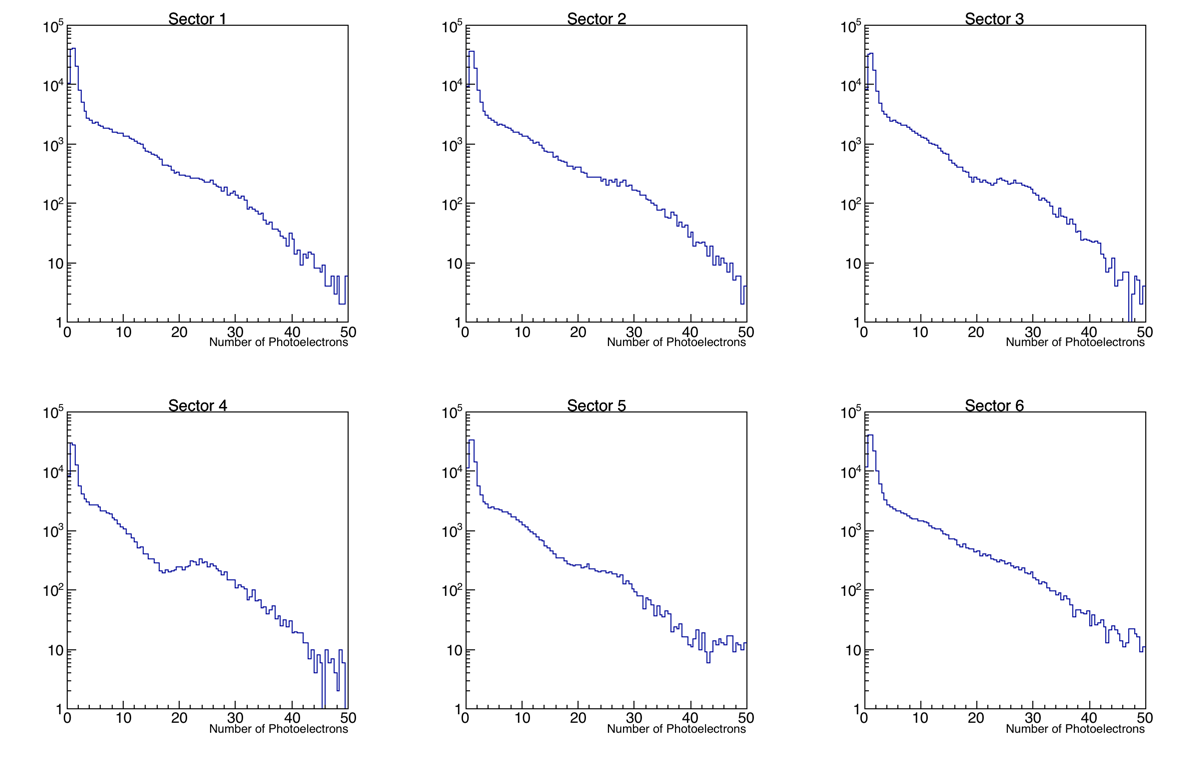
\includegraphics[width=0.75\textwidth]{figures/calib/cc/npeCC_check.png}
  \caption{An example CC photoelectron spectra from two production runs skimmed for pions.  The y-axis range is fixed over all plots for ease of comparison.}
  \label{calib.cc_pesec}
  \end{center}
\end{figure}

In Fig.~\ref{calib.cc_pepmt} the photoelectron yields are further broken down by PMT.  The z-axis (log-scale) is fixed for ease of comparison.  The important feature here is that the delta-ray "pion" peak in the photoelectron spectra peaks roughly around 1.0 photoelectrons for all PMTs. The general lepton selection criteria includes a cut > 2.5 photoelectrons, which is a relatively safe and conservative cut on any PMT (see Sec.~\ref{sec:data.lepton} for more details on the lepton PID).

\begin{figure}[htpb]
\begin{center}
 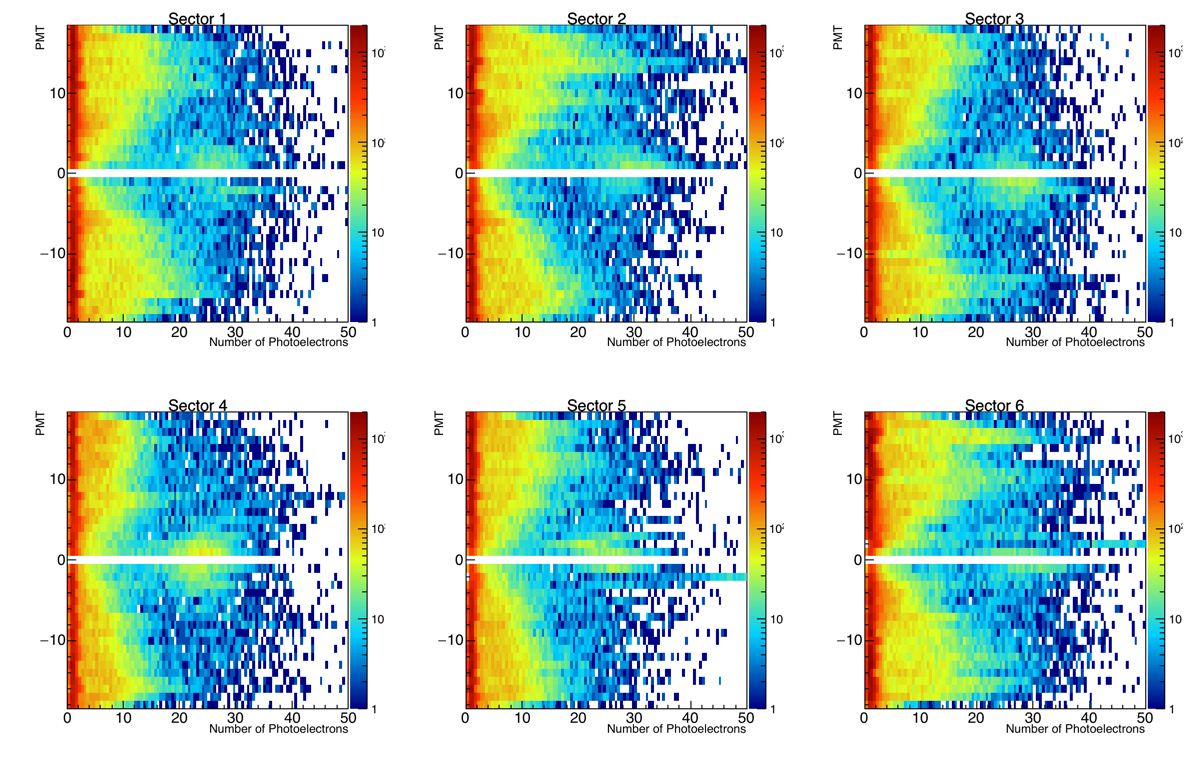
\includegraphics[width=0.75\textwidth]{figures/calib/cc/PMT_v_npe_log.png}
  \caption{Same plot as Fig.~\ref{calib.cc_pesec} but 2D in PMT number.  Negative and positive PMT numbers correspond to left and right CC PMTs. Z-axis range is fixed for ease of comparison.}
  \label{calib.cc_pepmt}
  \end{center}
\end{figure}

As an additional validity plot, the probability of a pion to cause a hit in the CC versus the momentum of the pion is shown in Fig.~\ref{calib.cc_piprob}.  This plot shows the expected behavior of the CC as the pions passes the Cerenkov radiation threshold.

\begin{figure}[htpb]
\begin{center}
 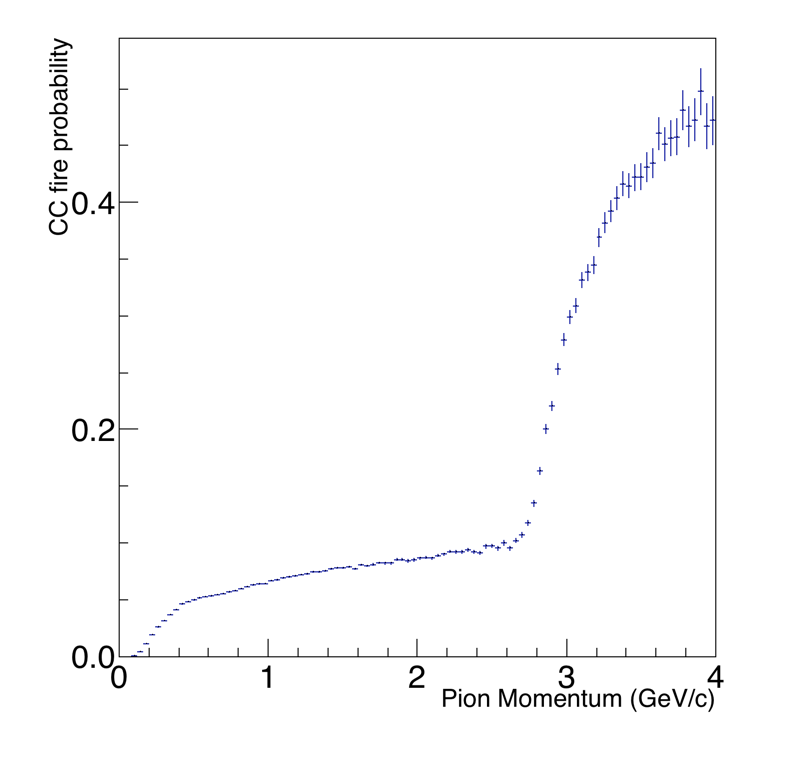
\includegraphics[width=0.45\textwidth]{figures/calib/cc/pionProb.png}
  \caption{The overall CC hit probability for pions within the fiducial region versus the pion momentum.}
  \label{calib.cc_piprob}
  \end{center}
\end{figure}

\subsubsection{\label{sec:calib.cc.eff}Cerenkov Efficiency}
The exact efficiency of the CC over all momenta and angles for leptons was never explicitly calculated.  Instead, it is recommended to look at the efficiency of the overall lepton identification procedure, if needed, for any lepton analyses.


\FloatBarrier

\subsection{\label{sec:calib.tof}Time-of-Flight Counter Calibration and Resolution}

\subsubsection{\label{sec:calib.tof.eff}Time-of-Flight Counter Efficiency and Bad Paddles}

As a standard procedure of the time-of-flight calibrations, the time-of-flight scintillators were initially studied during the calibration period, in which a list~\footnote{Can be obtained using the CLAS calibration database} of scintillators had a faulty ADC or TDC as shown in \ref{tab:craigtof}. Another study, as shown below, was conducted to determine the efficiency of each paddle and to reevaluate the status of their ADC and TDC. Due to the more stringent requirements of paddle efficiency in the study below, more paddles were considered to be faulty than in the initial study. \ref{tab:diff} shows the additional paddles which were considered to be inefficient.

\begin{table}
\begin{minipage}{\textwidth}
\begin{center}
\begin{singlespacing}

\caption{\label{tab:craigtof}List of faulty paddles as compiled during calibration}
    
\begin{tabular}{llp{.43\textwidth}}

\hline \hline

Sector & SCID & Notes \\

\hline

1 & 6 & No ADCR and TDCR \\
2 & 8 & No ADCL and TDCL \\
2 & 34 & No ADCL and TDCL \\
3 & 11 & No ADCR and TDCR \\
3 & 57 & No ADCL, ADCR, TDCL, and TDCR \\
4 & 48 & No ADCL and TDCL \\
5 & 57 & No ADCL, ADCR, TDCL, and TDCR \\
6 & 5 & No ADCR and TDCR \\

\hline \hline

\end{tabular}

\end{singlespacing}
\end{center}
\end{minipage}
\end{table}
 % label: tab:craigtof

\begin{figure}
    %\vspace{16pt}
    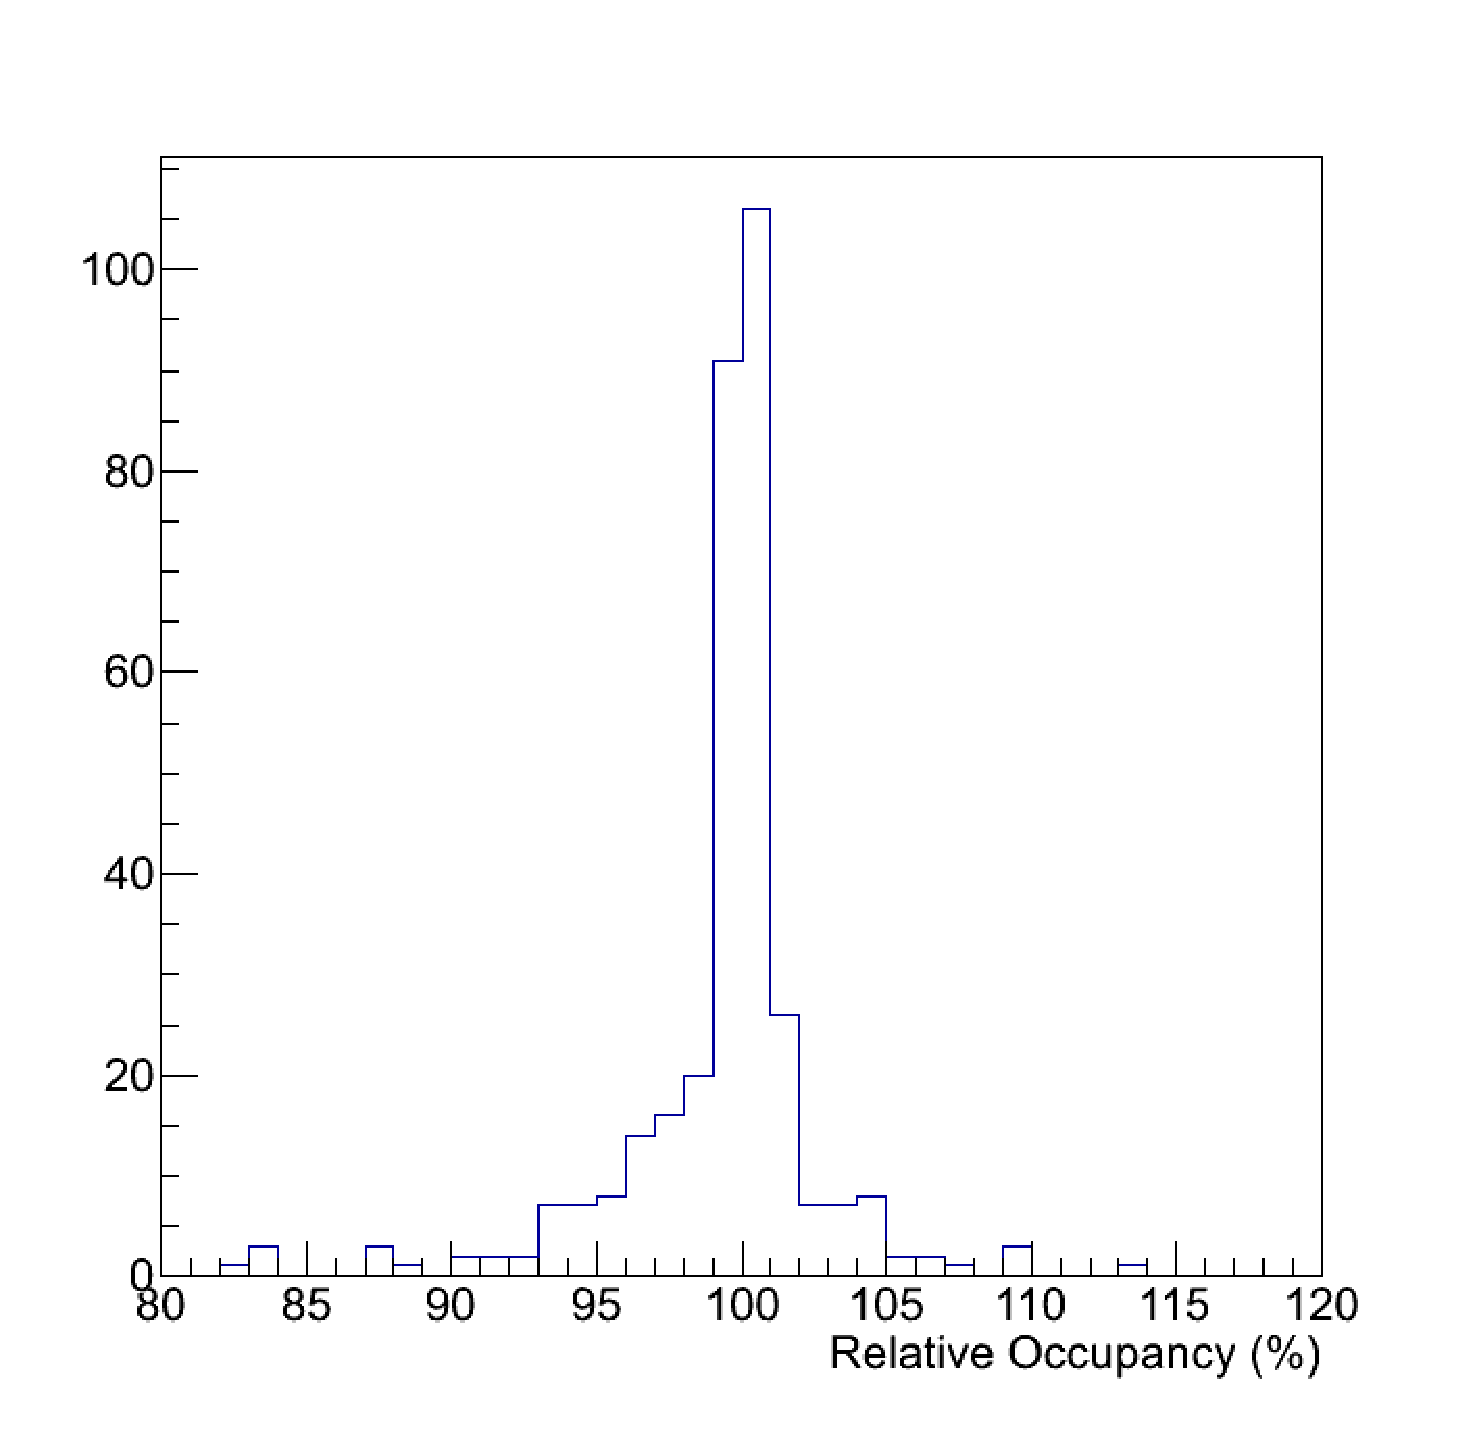
\includegraphics[trim=0 40 10 40,clip,width=.70\linewidth]{figures/calib/tof/tofko/occp.eps}
    \caption{Relative occupancy of all scintillators}
    \label{plt:occp}
\end{figure}

To determine efficiency of each scintillator paddle, the number of hits~\footnote{The data used were obtained from the \texttt{clas\underline{\hspace{5pt}}0$[$run\#$]$.A01} files located in \texttt{$/$mss$/$clas$/$g12$/$data$/$}} registered by every paddle was recorded~\footnote{This was done by using \texttt{bosdump -GSC} and parsing its output}. The relative occupancy of paddle $i$ in sector $j$ is defined the following way: list the number of hits recorded by all paddle $i$'s in sectors $\neq j$ and remove the ones with the most and least hits from the list. Take the average number of hits of the remaining three paddles. The relative occupancy is defined as 
\[
100 \times \frac{ \mathrm{Number of hits in paddle } i \mathrm{ of sector } j}{\mathrm{Average of remaining three paddles}} \hspace{2pt}\%
\]

\ref{plt:occp} shows the relative occupancy of all scintillators plotted on a single histogram. A paddle is defined as inefficient if it is greater than two standard deviations below the mean relative occupancy of all scintillators. \ref{tab:occp} shows the paddles which are below two (left) or three (right) standard deviations below the mean relative occupancy.


\input{tables/tof_padpaddles_stddev} % label: tab:occp

\subsubsection{ADC and TDC Values}


\begin{figure}
    %\vspace{-16pt}
    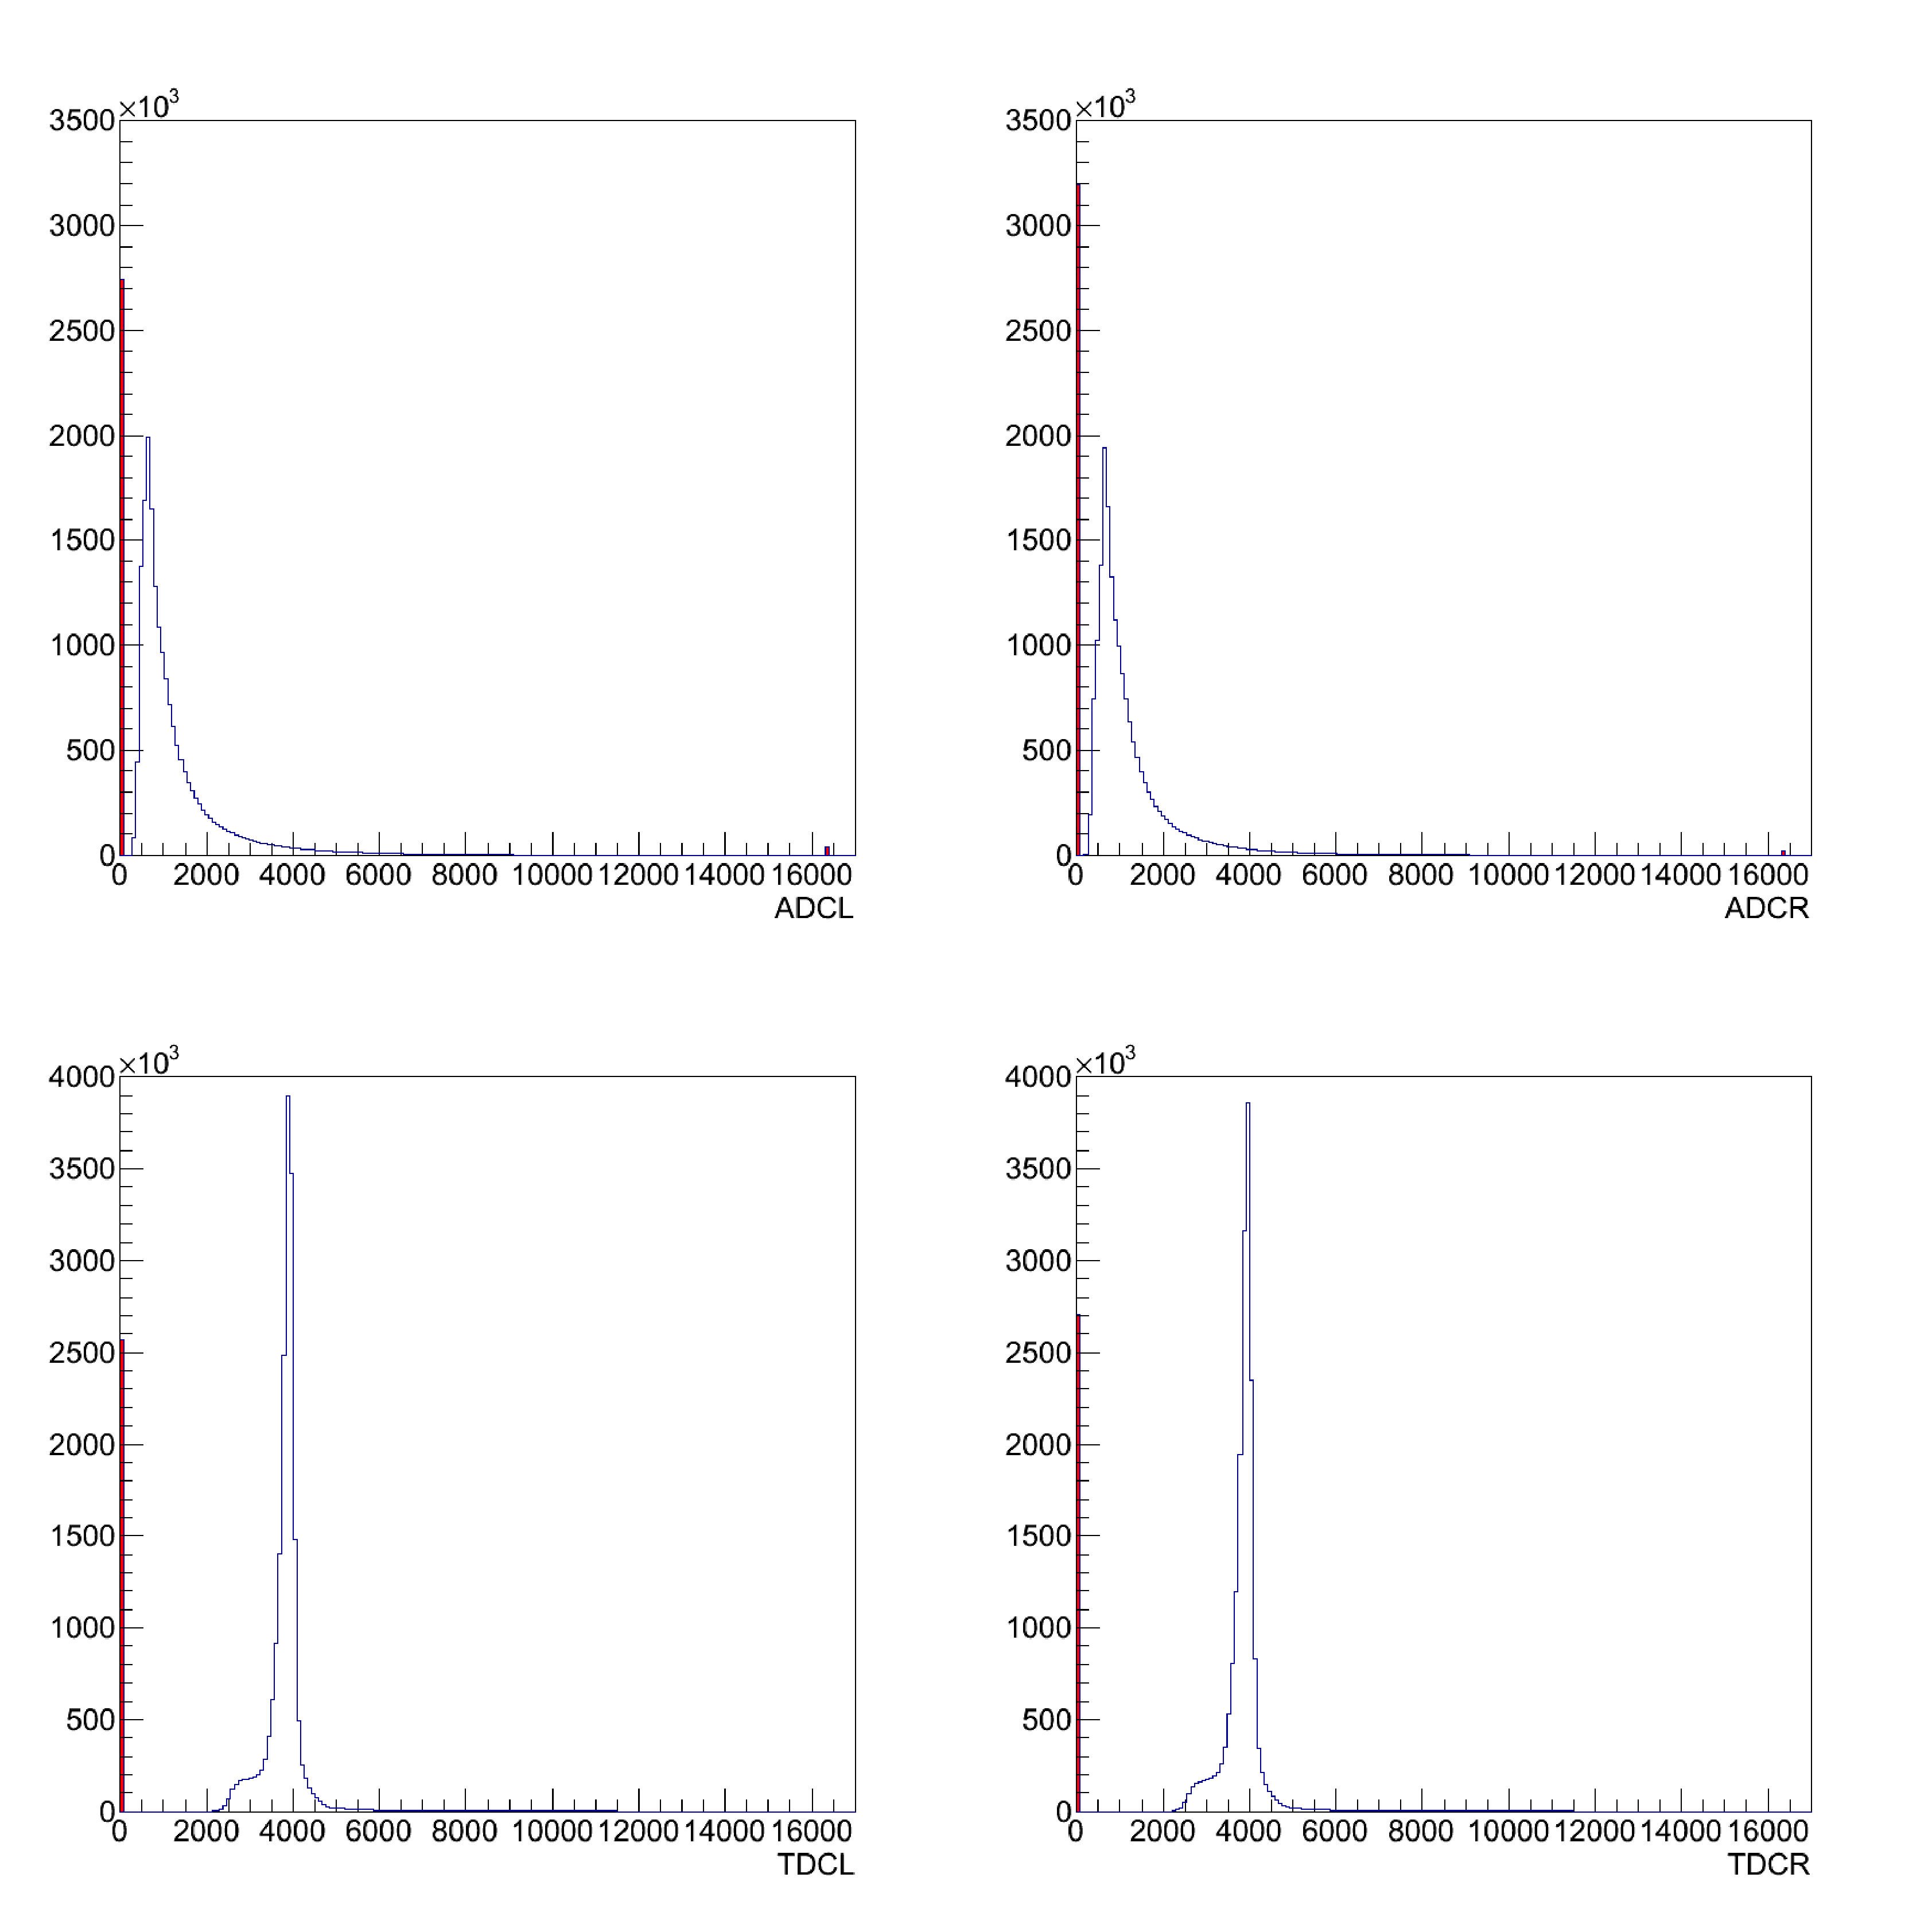
\includegraphics[width=0.70\linewidth]{figures/calib/tof/tofko/adctdcval.eps}
    \caption{Top: ADC values of all scintillators. Left ADC (ADCL) values are on the left and right ADC values are on the right (ADCR). Shaded in red are events recorded with an ADC value of zero or maximum. Bottom: Same as Top but for TDC values}
    \label{plt:adctdcval}
\end{figure}


The occupancy alone is not enough to determine which scintillators are bad. The ADC and TDC values for all scintillators were also recorded and studied. \ref{plt:adctdcval} shows the ADC and TDC values for all scintillators. Some of the events registered had an ADC or TDC value of zero or a maximum ADC value (shaded in red). The percentage of events a scintillator recorded either a TDC or ADC value of zero or maximum ADC value was studied as shown in \ref{plt:adc0vSCID,plt:adcMvSCID,plt:tdc0vSCID}. \ref{plt:adc0vSCID,plt:tdc0vSCID,plt:proj} assisted in determining bad paddles. It (is to be) was decided that a paddle cannot have more than $50\%$ of its ADC (left or right) values be equal to zero or more than $45\%$ of its TDC (left or right) values equal to zero. \ref{tab:adctdc0} shows which paddles fall in these categories. \ref{tab:tofko} shows which scintillators should be knocked out due to low occupancy or too many null ADC or TDC values. Due to the small number of events in which a maximum ADC value is obtained, it is not recommended in knocking paddles out based on this measure. However, \ref{tab:adcM} shows the paddles which attain a maximum ADC value on more than $2.5\%$ of its registered events.


\begin{table}
\begin{minipage}{\textwidth}
\begin{center}
\begin{singlespacing}

\caption{\label{tab:adctdc0}Paddles which registered an ADC or TDC value of zero greater than 50\% and 45\%, respectively, of its entries}

\begin{tabular}{lp{.43\textwidth}p{.43\textwidth}}

\hline \hline

 &  \% Events with ADCL or ADCR = 0 \( > \) 50\% &  \% Event with TDCL or TDCR = 0 \( > \) 45\% \\
 
\hline

Sector 1 & 6 (100\% ADCR) & 6 (100\% TDCR), 46 (97.89\% TDCL), 50 (98.11\% TDCL) \\
Sector 2 & 8 (100\% ADCL), 34 (100\% ADCL), 44 (50.22\% ADCL), 54 (52.00\% ADCR) &  8 (100\% TDCL), 34 (100\% TDCL), 44 (47.51\% TDCL), 54 (47.10\% TDCR)\\
Sector 3 & 11 (100\% ADCR), 56 (74.75\% ADCR) & 11 (100\% TDCR), 56 (62.79\% TDCR)\\
Sector 4 & 48 (100\% ADCL) & 48 (100\% TDCL) \\
Sector 5 & 48 (77.98\% ADCL) & 48 (76.10\% TDCL)\\
Sector 6 & 5 (100\% ADCR), 56 (59.30\% ADCR) & 1 (98.78\% TDCL), 5 (100\% TDCR), 33 (97.78\% TDCL) \\

\hline \hline

\end{tabular}

\end{singlespacing}
\end{center}
\end{minipage}
\end{table}
 % label: tab:adctdc0

\begin{table}
\begin{minipage}{\textwidth}
\begin{center}
\begin{singlespacing}

\caption{\label{tab:tofko}Union of \ref{tab:occp,tab:adctdc0} (Recommended list of paddles to knockout)}

\begin{tabular}{lc}

\hline \hline

Sector 1: & 6, 35, 40, 41, 50, 56\\
Sector 2: & 2, 8, 34, 35, 41, 44, 50, 54, 56\\
Sector 3: & 11, 35, 40, 41, 56\\
Sector 4: & 41, 48 \\
Sector 5: & 48\\
Sector 6: & 1, 5, 33, 56 \\

\hline \hline

\end{tabular}

\end{singlespacing}
\end{center}
\end{minipage}
\end{table}

 % label: tab:tofko


\begin{table}
\centering
\begin{tabular}{l | c |}
Sector 1 & 35, 40, 41, 50, 56 \\
Sector 2 & 2, 35, 41, 44, 50, 54, 56 \\
Sector 3 & 35, 40, 41, 56 \\
Sector 4 & 41 \\
Sector 5 & 48 \\
Sector 6 & 1, 33, 56
\end{tabular}
\caption{Paddles in \ref{tab:tofko} not included in \ref{tab:craigtof}}
\label{tab:diff}
\end{table}

\begin{table}
\centering
\begin{tabular}{l | c |}
Sector 1 & 20 (2.93\% ADCL)\\
Sector 3 & 20 (4.26\% ADCL)
\end{tabular}
\caption{Paddles with percentage of hits registering a maximum ADC value \( > \) 2.5\% of its events}
\label{tab:adcM}
\end{table}

\begin{figure}
    %\vspace{-16pt}
    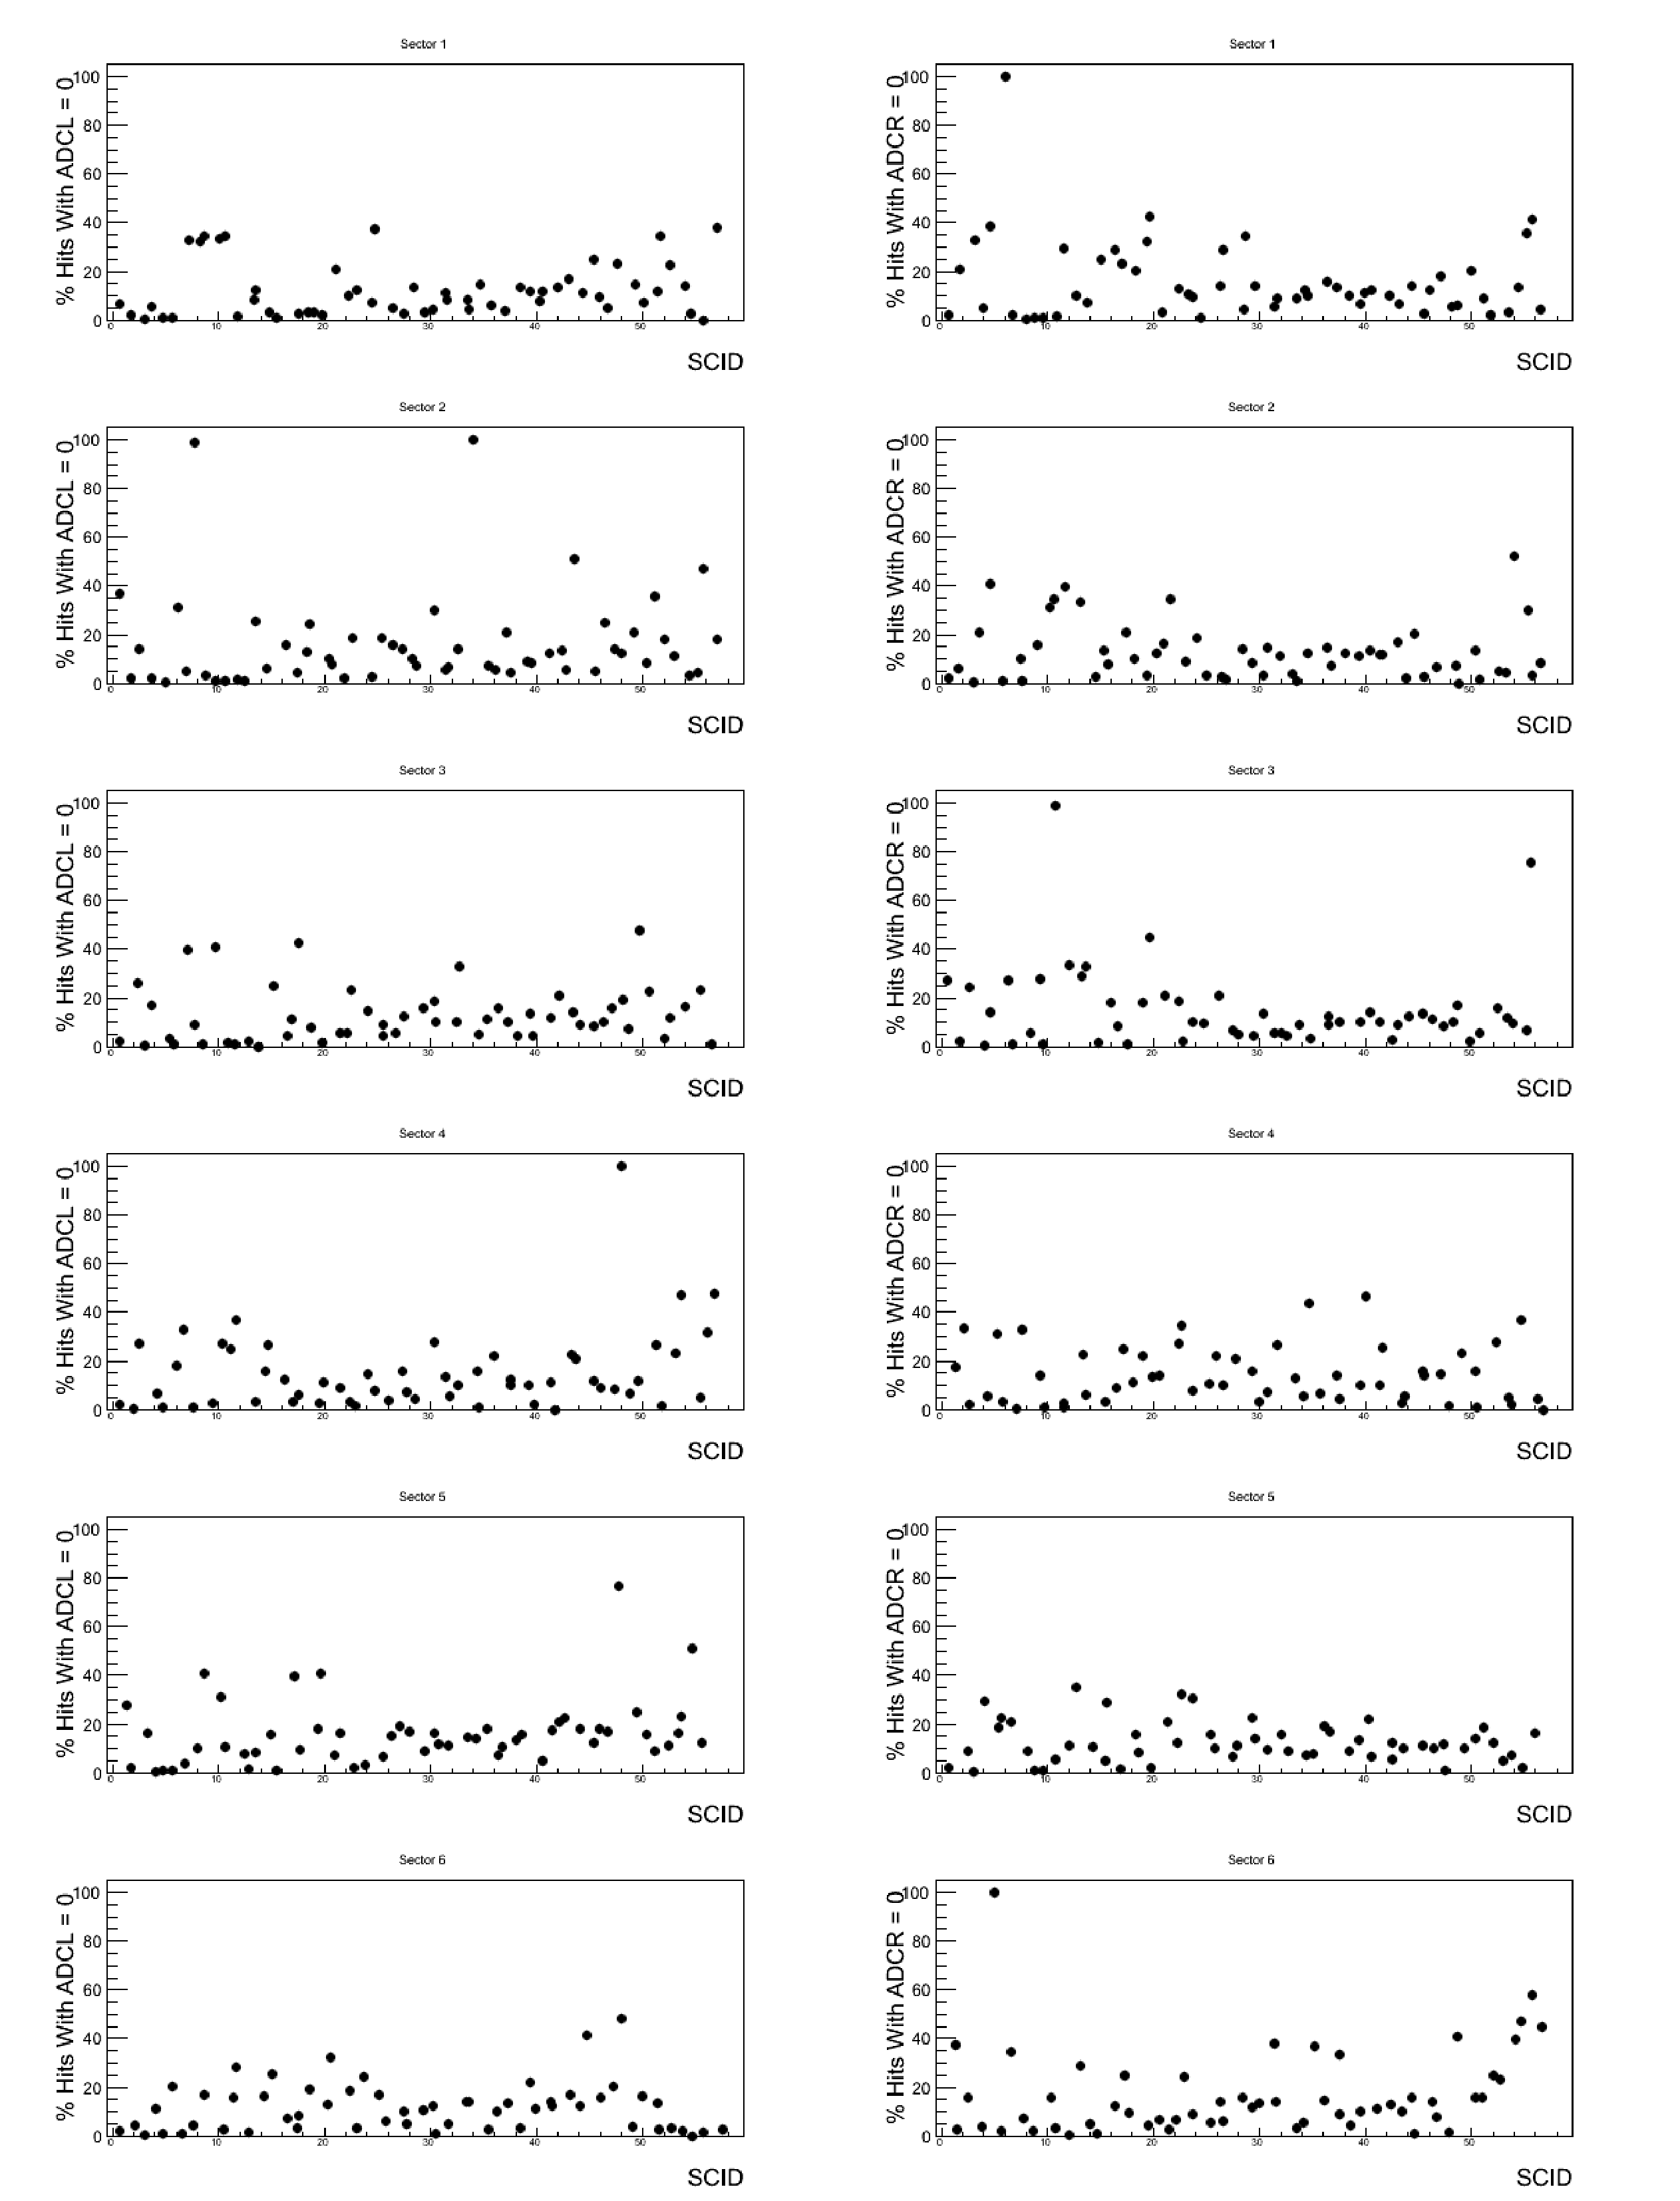
\includegraphics[width=0.8\textwidth]{figures/calib/tof/tofko/adc.eps}
    \caption{Percentage of hits registering an ADC value of 0 for all scintillators. Left ADC (ADCL) are on the left and right ADC (ADCR) values are on the right}
    \label{plt:adc0vSCID}
\end{figure}

\begin{figure}
    %\vspace{-16pt}
    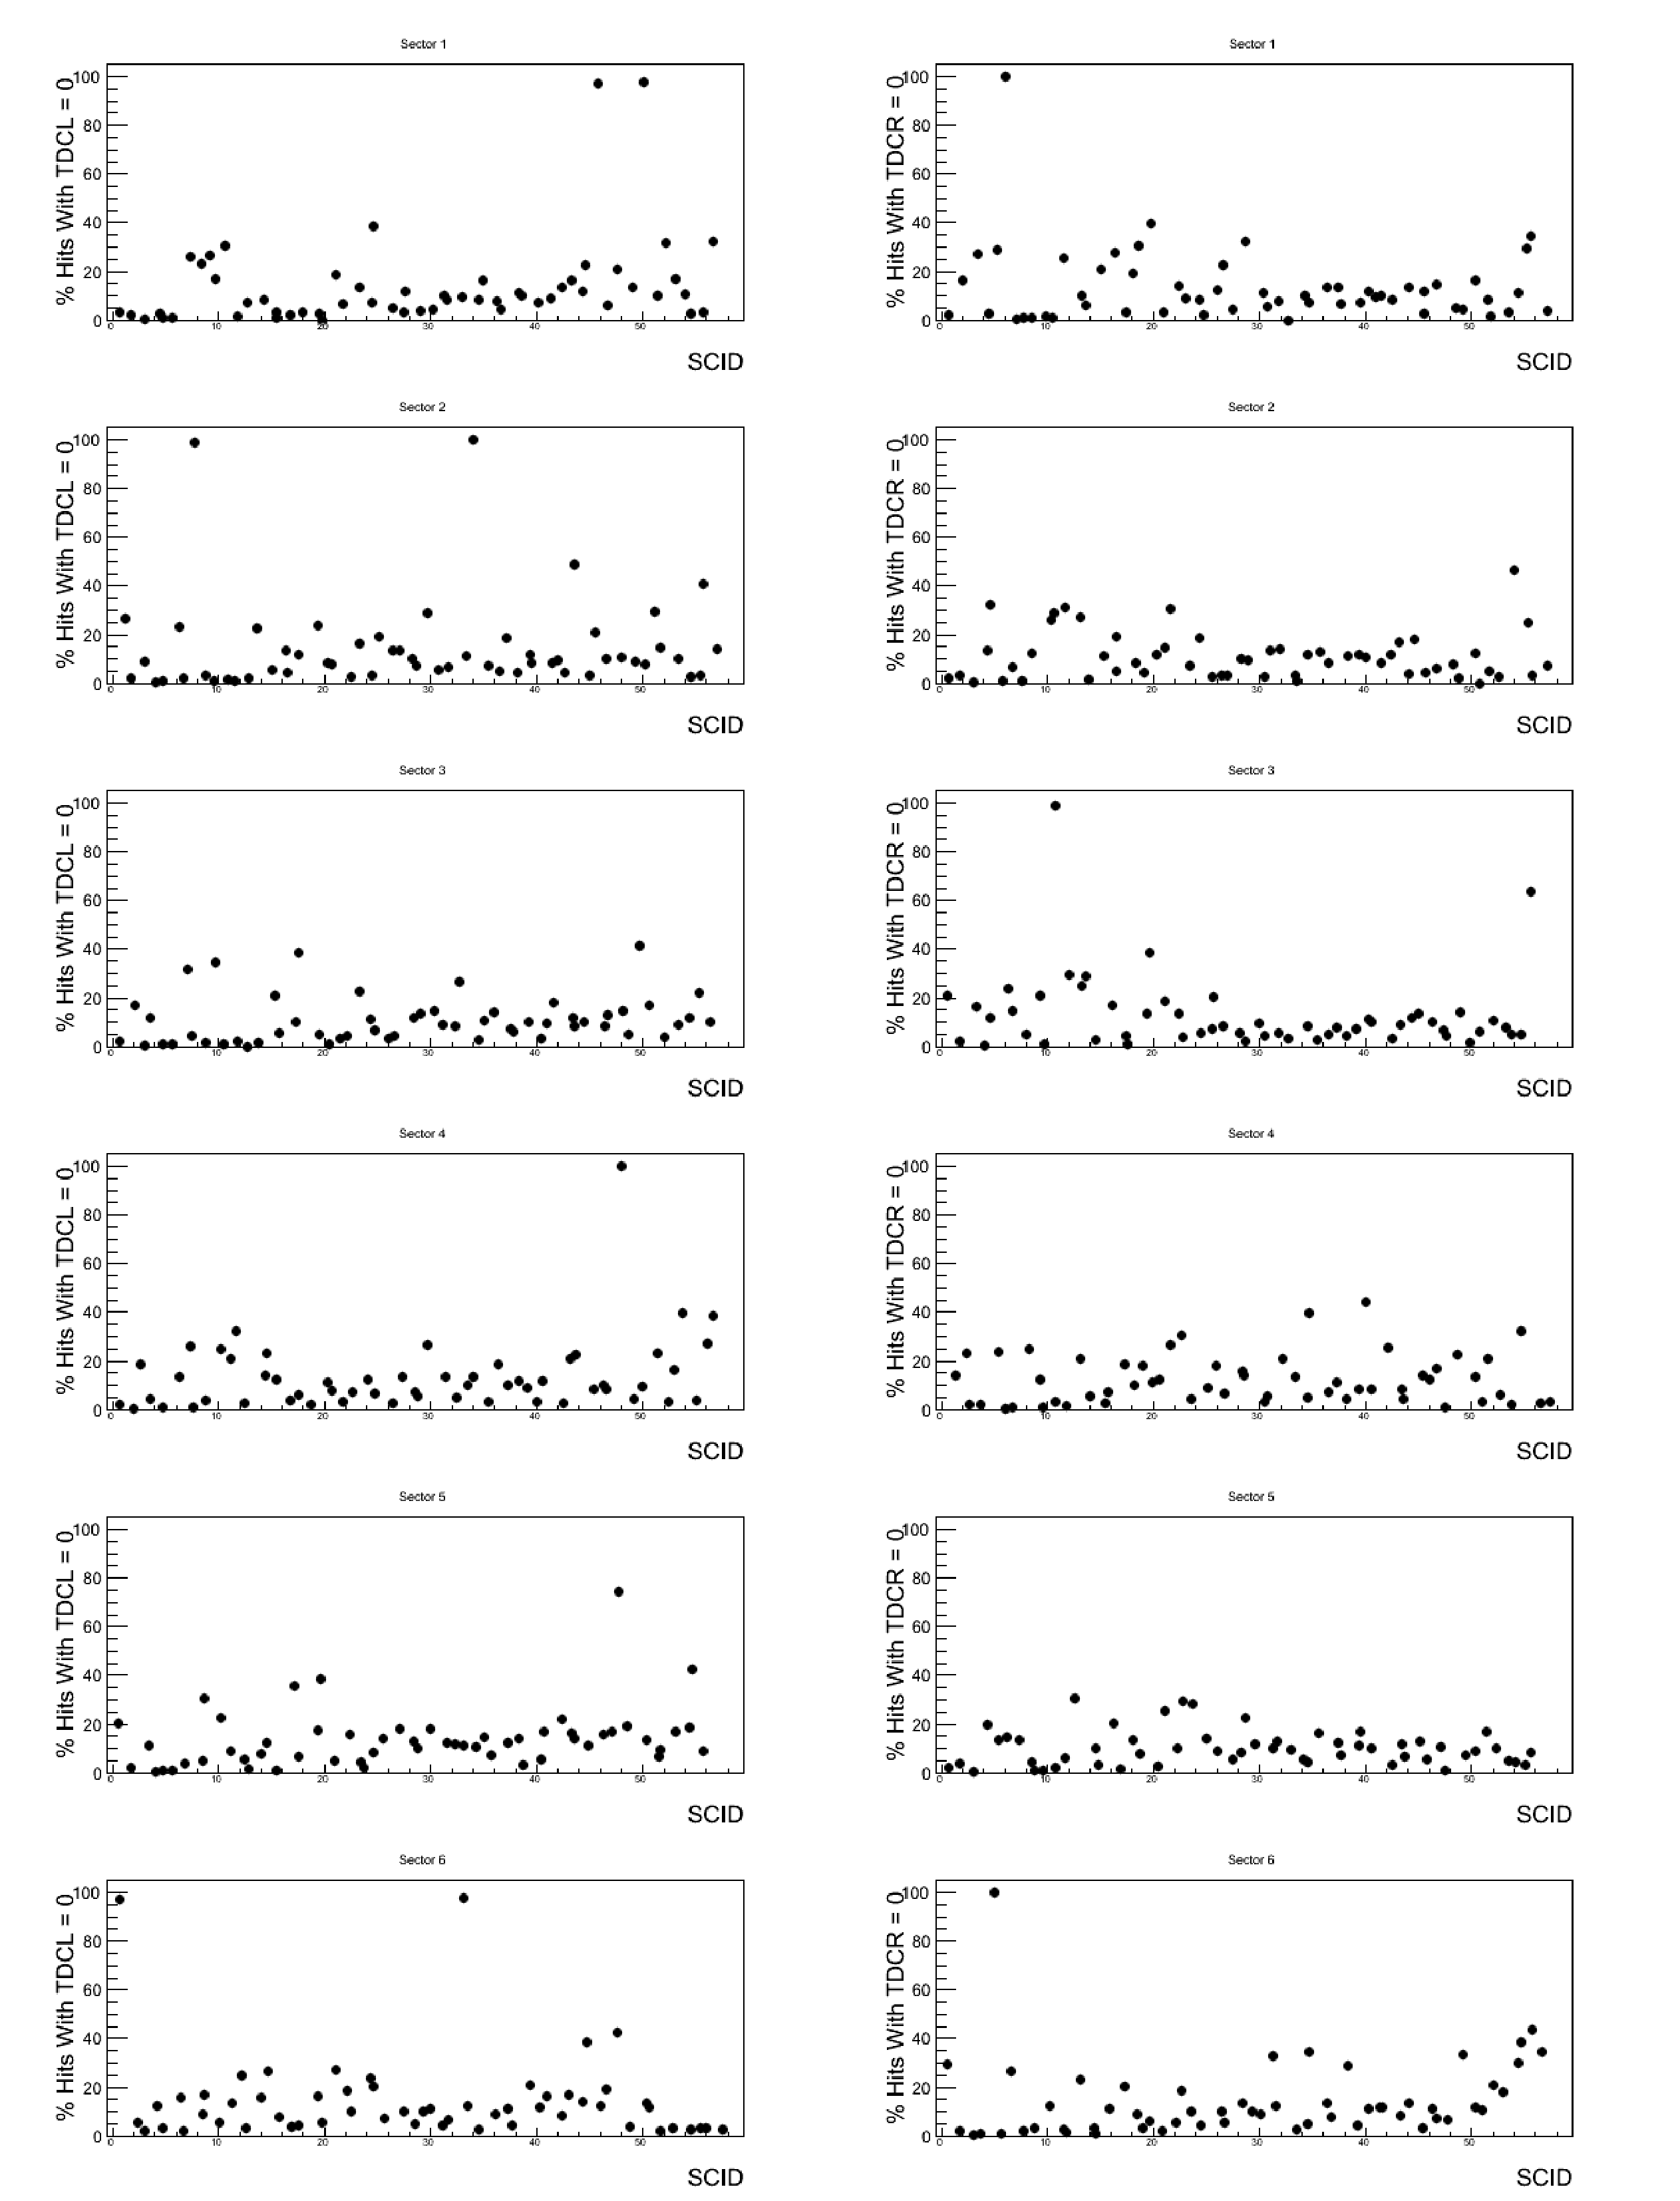
\includegraphics[width=0.8\textwidth]{figures/calib/tof/tofko/tdc.eps}
    \caption{Percentage of hits registering an TDC value of 0 for all scintillators. Left TDC (TDCL) are on the left and right TDC (TDCR) values are on the right}
    \label{plt:tdc0vSCID}
\end{figure}

\begin{figure}
    %\vspace{-16pt}
    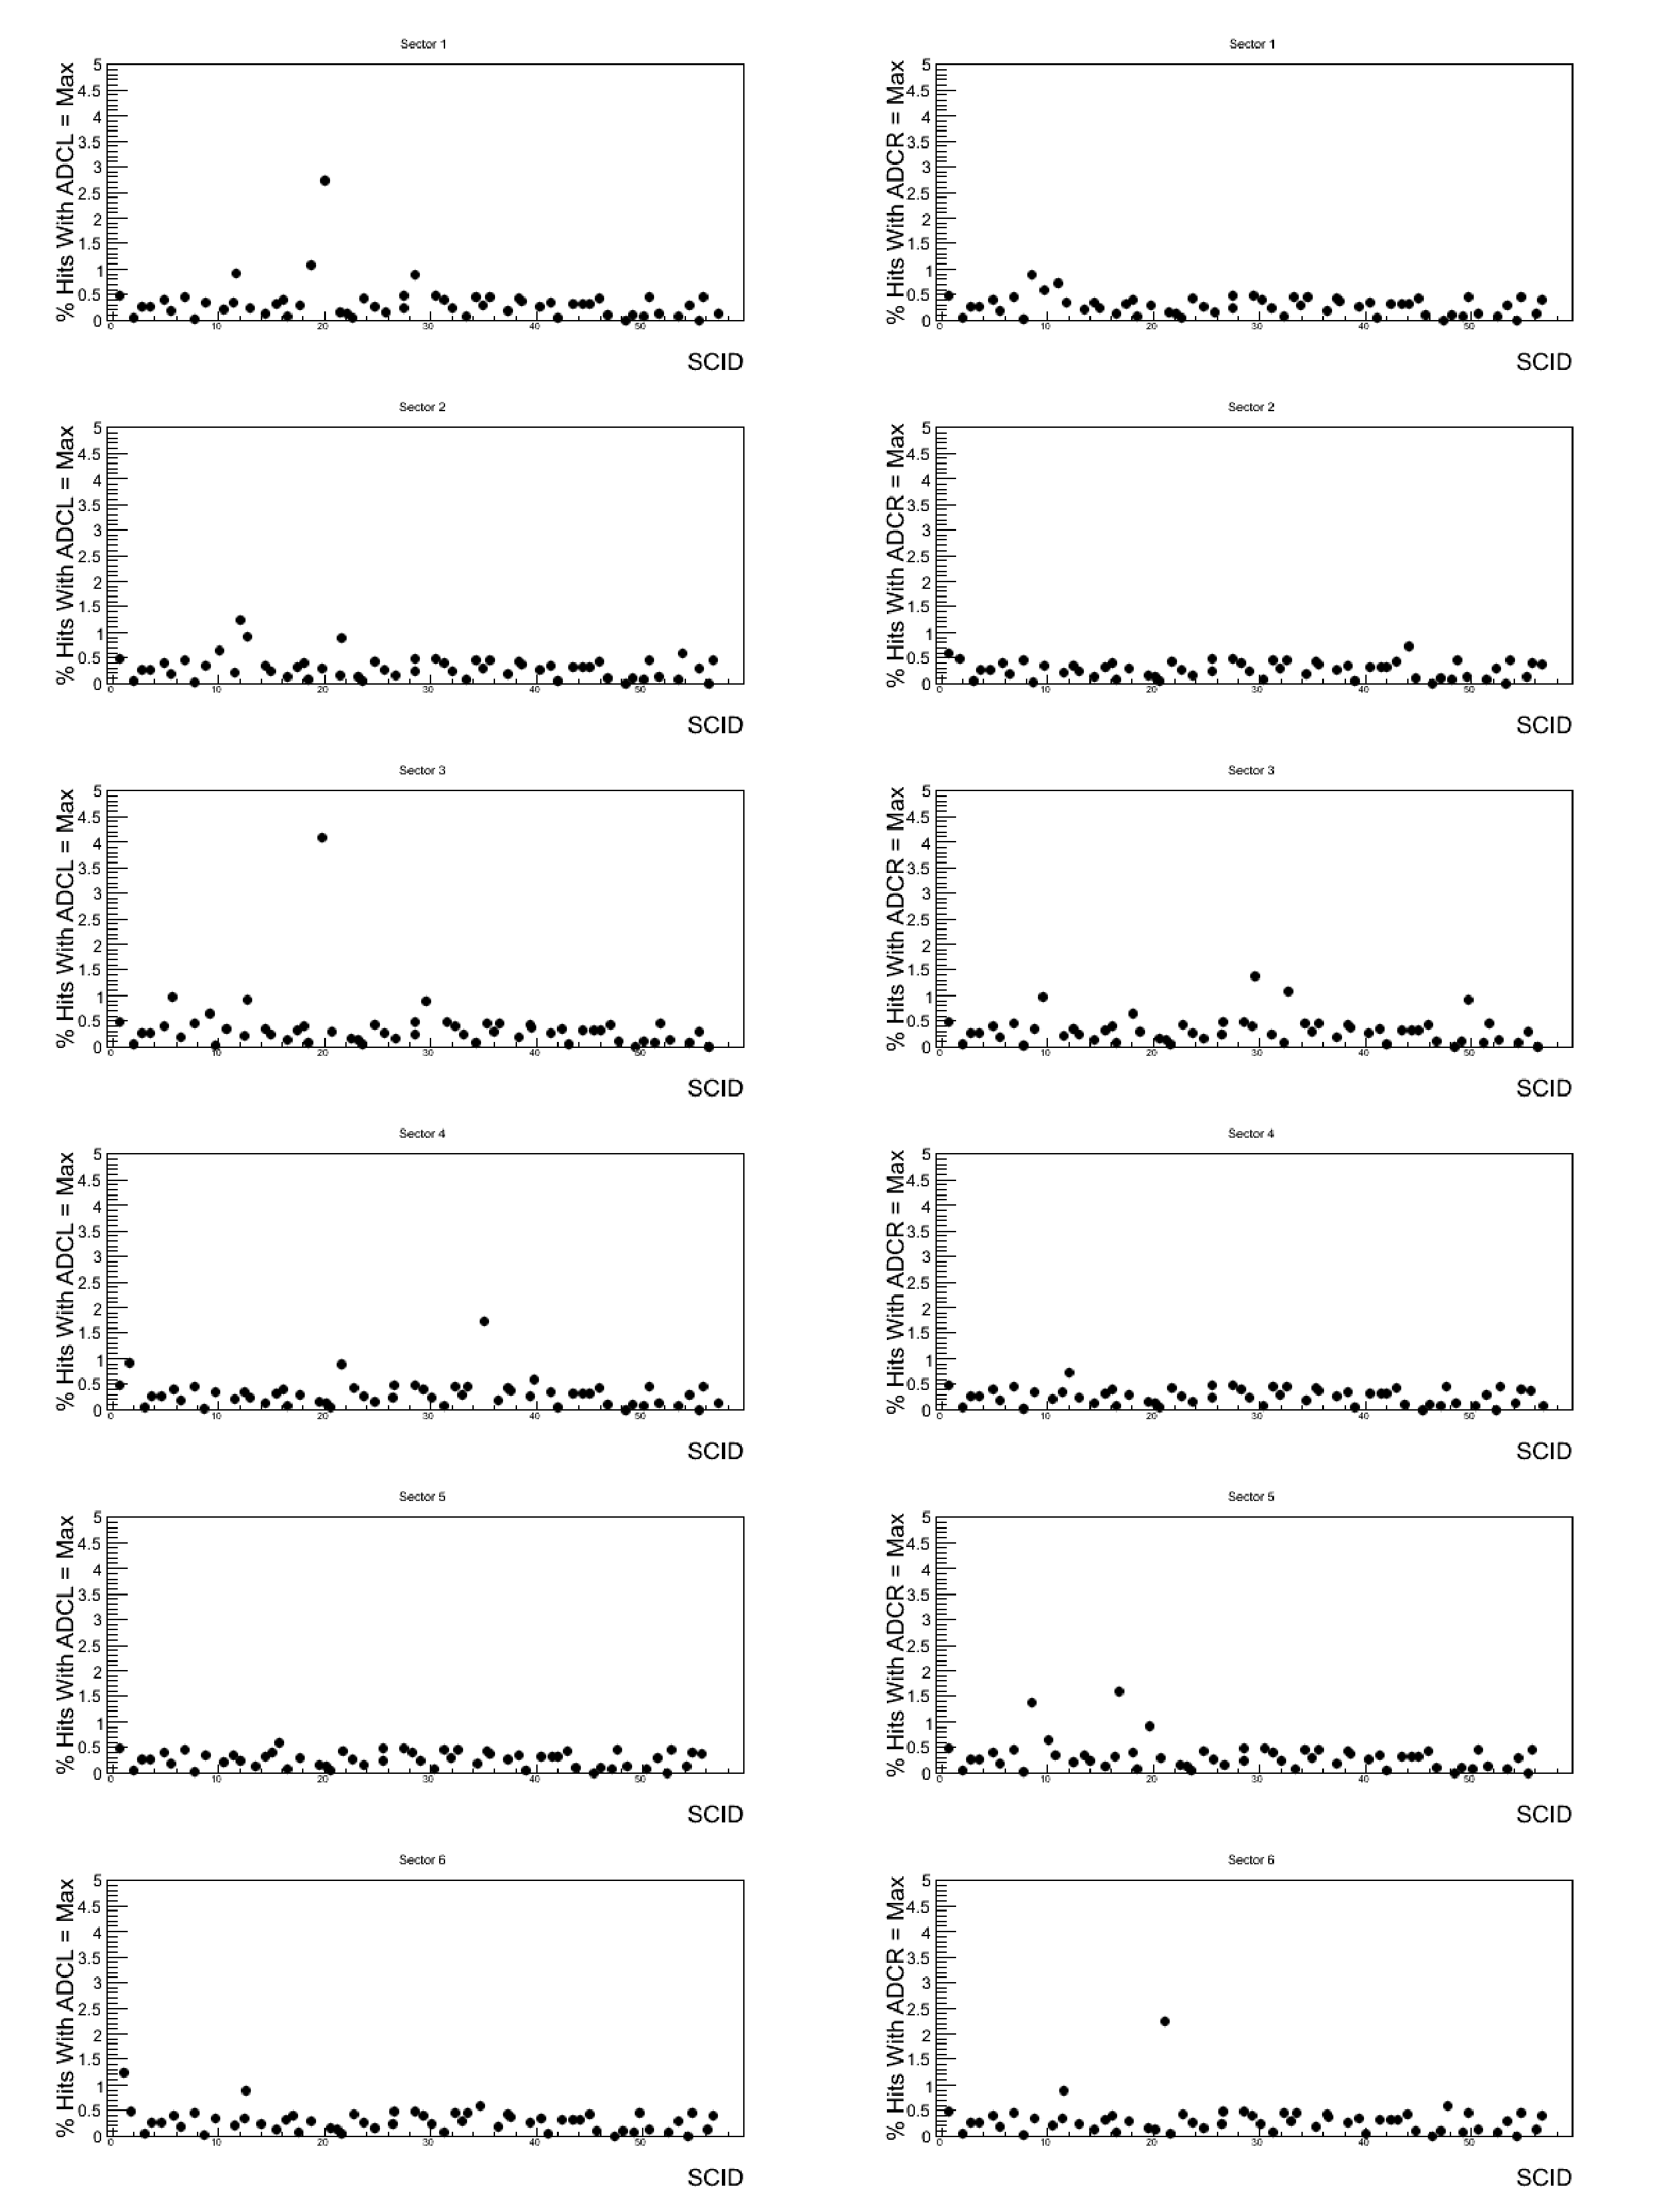
\includegraphics[width=0.8\textwidth]{figures/calib/tof/tofko/adcMax.eps}
    \caption{Percentage of hits registering a maximum ADC value for all scintillators. Left ADC (ADCL) are on the left and right ADC (ADCR) values are on the right}
    \label{plt:adcMvSCID}
\end{figure}

\begin{figure}
    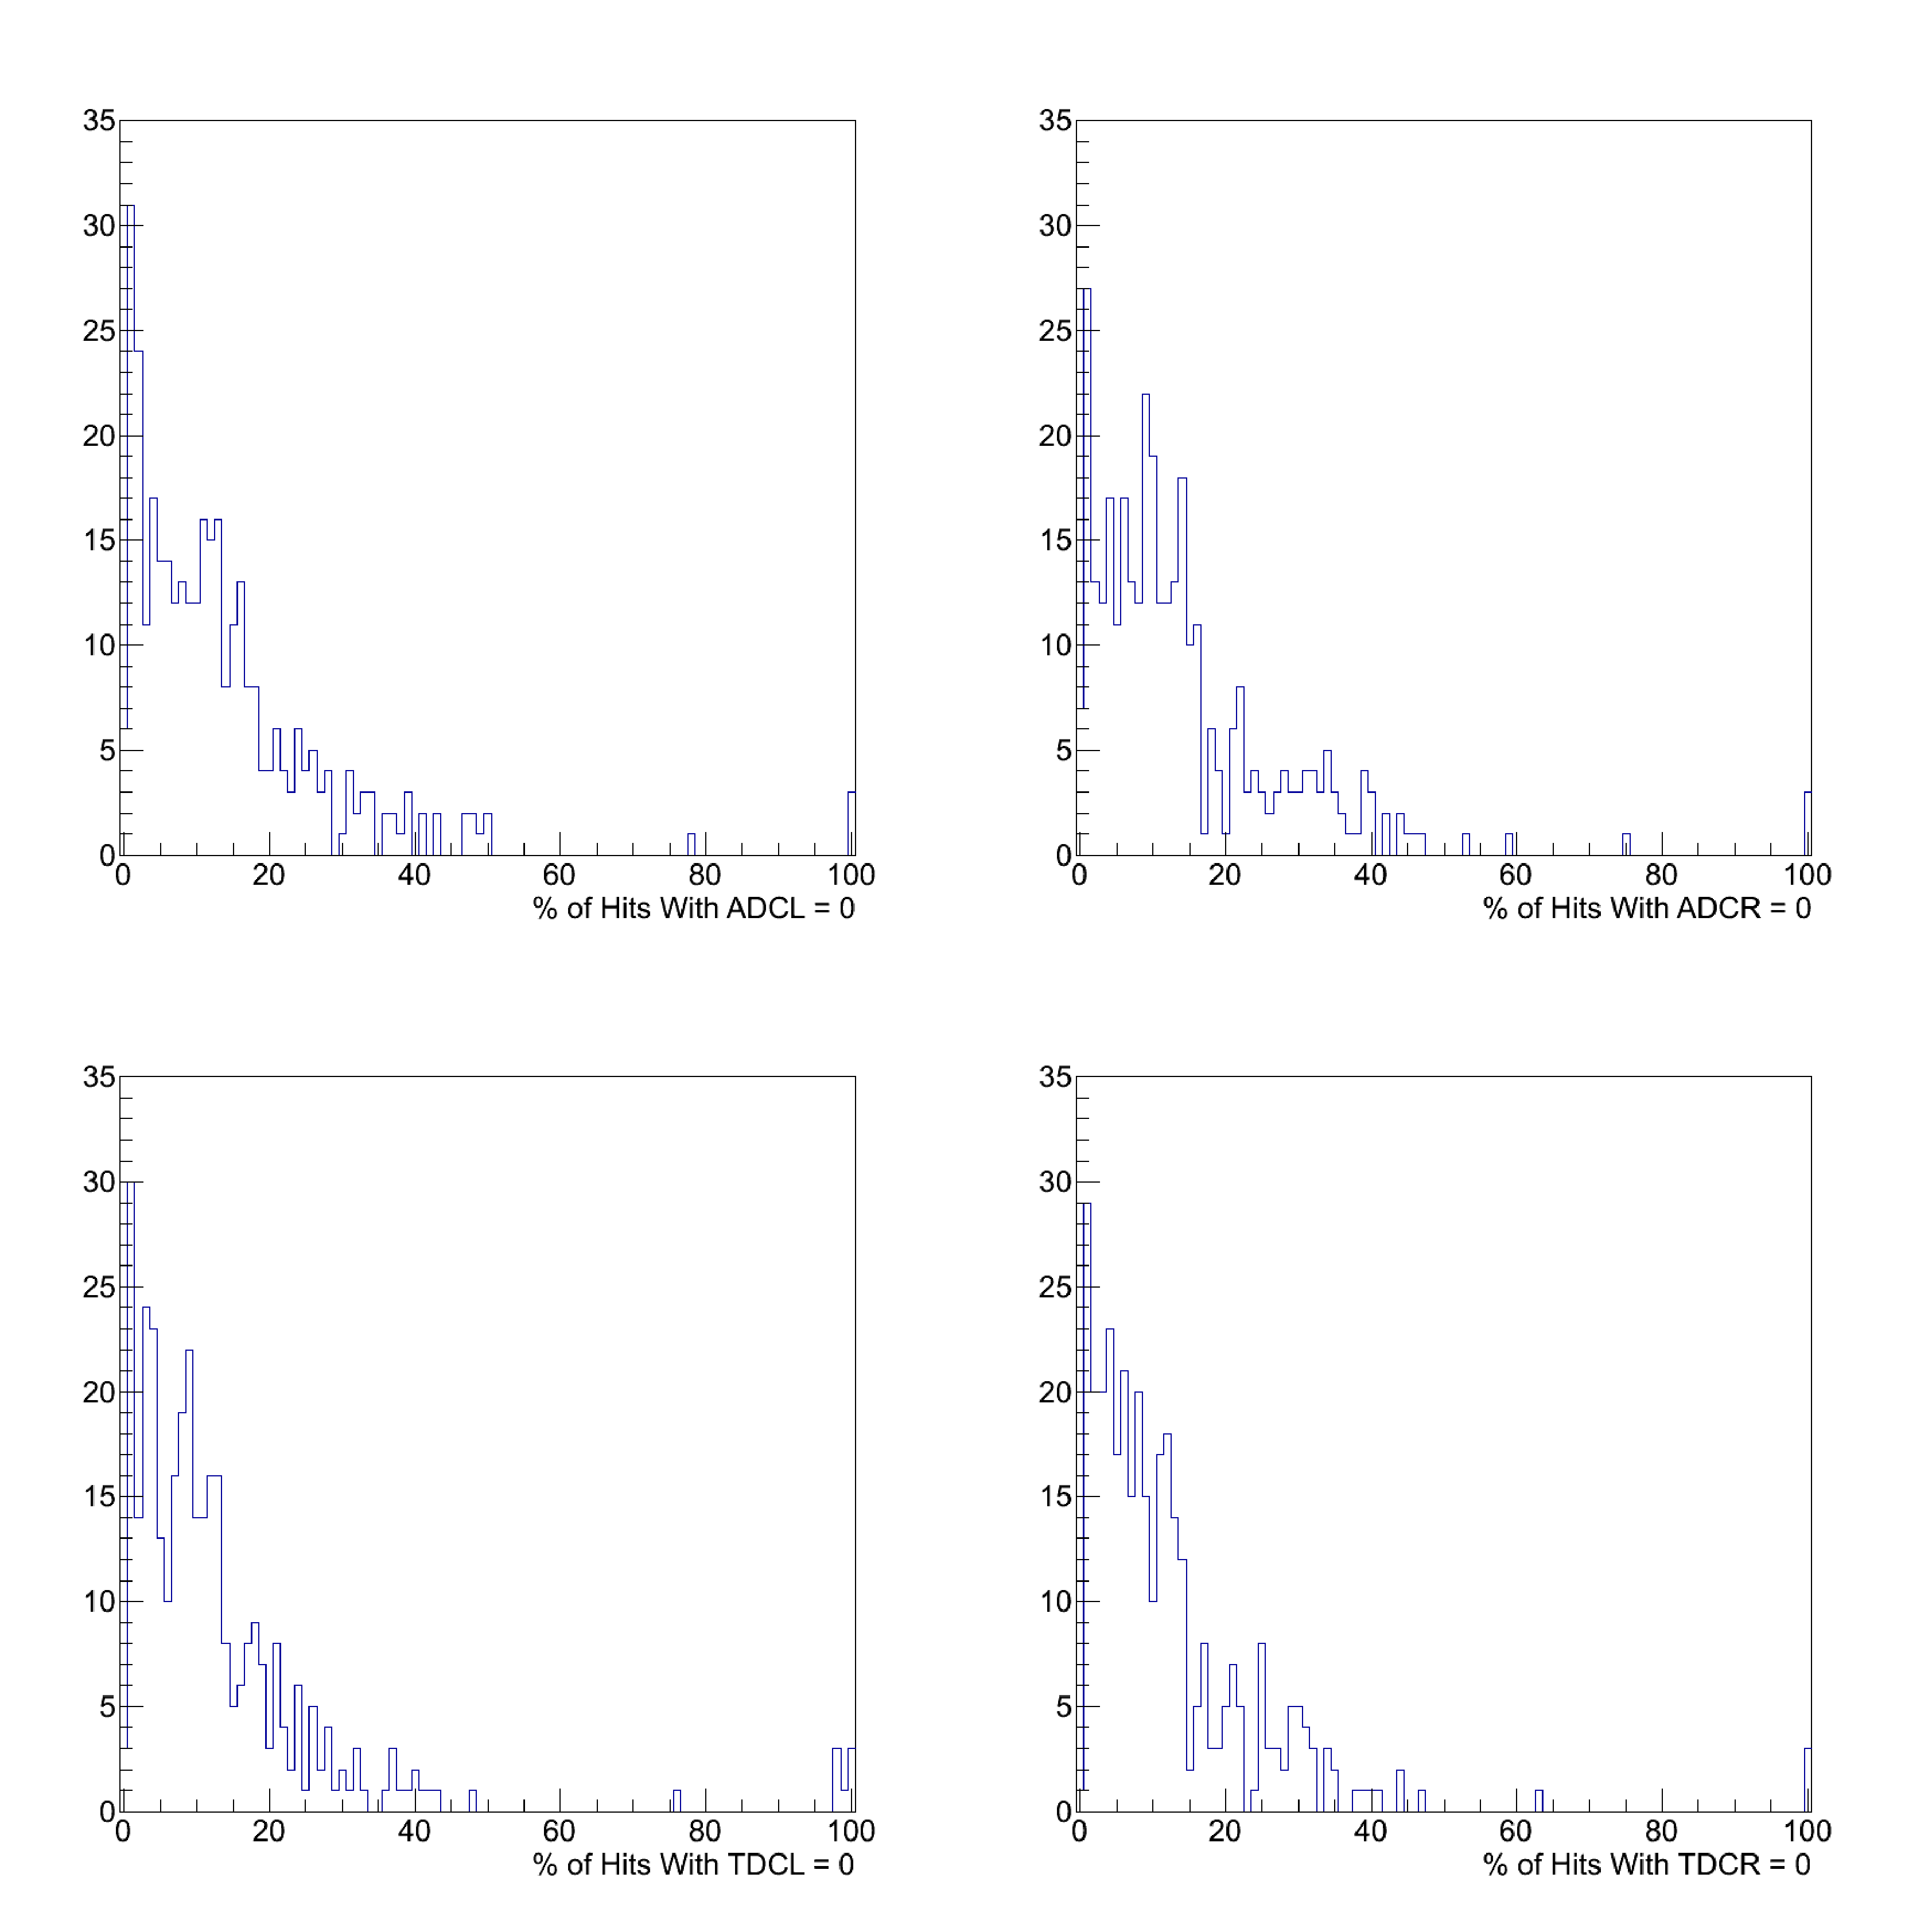
\includegraphics[width=0.8\textwidth]{figures/calib/tof/tofko/adctdc0perc.eps}
    \caption{Top: Y axis projections of \ref{plt:adc0vSCID}. Bottom: Y axis projections of \ref{plt:tdc0vSCID}}
    \label{plt:proj}
\end{figure}

\FloatBarrier

\subsection{\label{sec:calib.ec}Electrocalorimeter}

\subsubsection{\label{sec:calib.ec.eff}Electrocalorimeter Efficiency}

\FloatBarrier


\section{Analysis Procedure}

There was only one ``physics'' pass of the \desg{g12} data, labeled \texttt{pass1}, which represents 99\% of the reconstructable data taken. It was determined that tracking down that last 1\% was not worth the effort. On JLab's common user environment (\texttt{CUE}), the cooked data here:
\begin{center}
    \texttt{/mss/clas/g12/production/pass1/bos}
\end{center}
and the raw data can be found here:
\begin{center}
    \texttt{/mss/clas/g12/data/}
\end{center}

The broad steps for analysis of a specific reaction in the \desg{g12} data are:
\begin{enumerate}
    \item determine event selection cuts to be used on a small subset of the data,
    \item skim the ``cooked'' data and produce an ntuple which will include the four-momenta and a few other parameters needed for the final analysis,
    \item tune the analysis on the data to get the final yields,
    \item run simulations through the tracker/digitizer (\prog{gsim}), smearing (\prog{gpp}), track reconstruction (\prog{a1c}), and the final analysis programs to obtain efficiencies and acceptances,
    \item calculate the beam flux corresponding to the data analyzed,
    \item tie the yields, acceptances and flux together to come up with a final answer and an absolute scaling.
\end{enumerate}
One or more of these steps, or parts of these steps, may not be necessary for a given analysis and they do not have to be done this order. This section discusses where to find the various programs and files needed for each of these steps.

\subsection{\label{sec:ana.data}Obtaining Final-State Particle Data}

All reconstructed data resides in BOS files on the tape-silo at JLab under the directory:
\begin{align}
\texttt{/mss/clas/g12/production/pass1/bos} \nonumber
\end{align}
which contains the following subdirectories or ``categories'' used for event-sorting:
\begin{description}
    \item[1-1ckaon1ctrk] Events which have at least 2 charged tracks, one of which is a ``possible kaon.'' A possible kaon is either a track that the \abbr{PART} bank says is a kaon, or a high-momentum charged pion ($> 2.0$~GeV), or a really high momentum proton ($> 3.0$~GeV). The idea of this selection is to leave no kaon behind.
    \item[2-2pos1neg\_not\_1ckaon1ctrk] Two-positive and one-negative ($++-$) inclusive events which are \emph{not} included in \emph{1-1ckaon1ctrk}. So, for example, if you wanted all ($++-$) events you would have to use both this category and \emph{1-1ckaon1ctrk}.
    \item[3-2ctrk\_not\_2pos1neg\_1ckaon1ctrk] Events with 2 or more charged tracks which do not qualify for either \emph{1-1ckaon1ctrk} or \emph{2-2pos1neg\_not\_1ckaon1ctrk}.
    \item[4-not\_2ctrk\_2pos1neg\_1ckaon1ctrk] Physics events that do not fit into categories 1, 2, or 3.
    \item[5-other] Non-physics events which may include scalers and such.
    \item[6-1lepton] Redundant set of all events with a single ``possible lepton'' according to the
    \begin{align}
        \texttt{ClasParticle::isMaybeLepton()} \nonumber
    \end{align}
    method in the ClasEvent analysis suite.
    \item[7-4ctrk] Redundant set of all four-charged track events.
    \item[8-ppbar] Redundant set of all proton, anti-proton events according to the PART bank.
\end{description}
Note that the first five of these categories are \emph{mutually exclusive and complete} while the last three are completely redundant and are provided for convenience.

\paragraph{This bears repeating since it is a non-standard sorting of the cooked data:} The five categories numbered 1 through 5 listed above consist of one and only one of \emph{every} event recorded by the data aquisition during the g12 run period for the set of run which were deemed ``good.'' A specific single event will only be found in one of the first five categories. If you want to run on events that are described by category number 4 for example, you will have to include the data in categories 1 through 3 since these will also satisfy category 4 by design and by definition.

Typical analyses with \desg{g12} will start with the particles as identified in the \abbr{PART} bank as default in the \prog{ClasEvent} analysis suite. This provides the basic four-momenta of the tracks and their identification which is based on mass calculated from the time-of-flight. The photon associated with the event is then taken from the \abbr{TAGR} bank and the one closest in-time with the tracks is usually taken.

For a deeper analysis, one can get information for specific hits in a given subsystem by following the pointers in the \abbr{PART} and \abbr{TBID} bank to the \abbr{TBTR}, \abbr{SCRC}, \abbr{ECHB} or other similar banks. Most of the relavent banks needed for this type of investigation are included in the cooked data though several raw banks were dropped to save space. To recover the missing banks one would have to go back to the raw data and recook using the \prog{a1c} program though we anticipate this will be a rare event.


\subsection{Flux Determination}

The photon flux is based on the flux procedure outline in Ref. \cite{clas.flux.note}. The script to generate the photon flux for g12 is here:
\begin{align}
    \texttt{/home/clasg12/local/scripts/g12-gflux} \nonumber
\end{align} and there is also a script (/home/clasg12/local/scripts/g12-gflux-all) that doesn't rebin the energies and outputs two columns: energy and flux for each logical paddle in the tagger.

The help output from the script:
\begin{verbatim}
> /home/clasg12/local/scripts/g12-gflux -h
usage: g12-gflux emin emax ebinwidth runlist.txt (good|all)
    (good|all) specifies either all scalar intervals
    or only "good" scalar intervals.
example:
     g12-gflux 1.5 5.5 0.2 runlist.txt good
where runlist.txt is an ascii file of one column: run
56363
56365
...
\end{verbatim}

To use the script, you will need to create a file that consists of the run numbers you used in your analysis. Using this filename when you call g12-gflux, will give you the total flux as a function of beam energy in the range and binning requested. The command:
\begin{verbatim}
/home/clasg12/local/scripts/g12-gflux 1.5 5.5 0.2 filelist.txt good
\end{verbatim}

will return to stdout the flux in the energy bins using three columns: emin, emax, flux. Something like this:
\begin{verbatim}
1.5 1.7 7.75466725993e+12
1.7 1.9 7.23861294572e+12
1.9 2.1 6.85242336788e+12
... [snip] ...
4.9 5.1 2.69244768955e+12
5.1 5.3 2.49808049501e+12
5.3 5.5 1.99322166816e+12
\end{verbatim}

The option good or all can be used to specify if you only want to consider good regions, throwing out beam trips, or if you want all events from good scalar intervals as well as the beam trip regions.

An alternative script which doesn't rebin the data but returns the flux for each logical energy paddle can be run like this:
\begin{verbatim}
/home/clasg12/local/scripts/g12-gflux-all filelist.txt good
\end{verbatim}
The script has been extensively tested on the 64-bit machines. The precision of all variables are adequate to provide at least 4 significant figures for the final flux numbers.

The major caveat to using this script, which relies on \prog{gflux}, is that you must included \emph{whole runs} in your analysis for this to be accurate. This is because the \prog{gflux} program was not designed to work with partial runs. So, you must verify that you have processed every file in the runs which were analyzed -- one can use the \prog{g12runs} program to aid in this.


\FloatBarrier

\subsection{Reconstruction}

The reconstruction program \texttt{a1c} requires an environment variable to point to the correct run index for this run period. This can be set in a bash shell using the command:
\begin{verbatim}
export CLAS_CALDB_RUNINDEX=calib_user.RunIndexg12
\end{verbatim}
The command to cook the gsim bos file using the \texttt{a1c} program is:
\begin{verbatim}
a1c -T4 -sa -ct1930 -cm0 -cp0 -X0 -d1 -F -P0x1bff -z0,0,-90 \
  -Aprlink_tg-90pm30.bos -o3pi.a1c 3pi.gpp
\end{verbatim}
which will produce BOS files similar to the ``cooked'' data mentioned above in Sec.~\ref{ana.data}. This is the same command to be used to \emph{recook} raw data files.

\FloatBarrier


\subsubsection{General Features of Lepton Data in \desg{g12}}\label{sec:analysis.Lepton.general}

To identify electrons and positrons properly in \abbr{CLAS}, quantities obtained from the \abbr{CC} and \abbr{EC} are used to reject charged pions. The \abbr{CC} collects the number of photo-electrons caused by Cherenkov radiation and the \abbr{EC} records the energy deposition of electrons/positrons as well as photons. A previous \abbr{CLAS} experiment \desg{g7} analyzed the properties of medium modifications from the decay of vector mesons through the leptonic decay channel. This experiment derived a set of cits for identifying electron/positrons pairs in \abbr{CLAS} by employing specific cuts to the number of photo-electrons (\abbr{NPE}) detected in the \abbr{CC}, a match in azimuthal angle $\phi$ from a charged track in the \abbr{DC} to the $\phi$ of the \abbr{CC}, as well as comparing the momentum of the charged track to the energy deposited in the \abbr{EC}. These cuts can be found in Table~\ref{tab:ISLEP_cuts}.  
\begin{table}[h!]
\begin{minipage}{\textwidth}
\begin{center}
\begin{singlespacing}

\caption[Electron/Positron PID Cuts]{\label{tab:ISLEP_cuts}Cuts applied to the \emph{CC} and \emph{EC} to perform electron/positron \emph{PID}. Table source:~\cite{clas.thesis.kunkel} \vspace{0.75mm}}

\begin{tabular}{c|c|c}

\hline
Subsystem & Quantity & Cut \\
\hline
\multirow{2}{*}{\emph{CC}}  & \# of photo-electrons (\emph{NPE})  & \emph{NPE} $>$ 2.5 \\
 &  \emph{DC} $\phi$ \& \emph{CC} $\phi$  & \emph{DC} $\phi$ = \emph{CC} $\phi$ \\
\hline
\multirow{2}{*}{\emph{EC}}  & q$^{\pm}$ momentum threshold (p$\mathrm{_{thres}}$) & \multirow{2}{*}{p$\mathrm{_{thres}^{high}} < \ $E$\mathrm{_{calo}} <$ p$\mathrm{_{thres}^{low}}$ } \\
&  \& \emph{EC} deposited energy (E$\mathrm{_{calo}}$) & \\
\hline \hline
\end{tabular}
\end{singlespacing}
\end{center}
\end{minipage}
\end{table}

To validate the \desg{g7} electron/positron \abbr{PID} scheme for \desg{g12}, a comparison of  the \abbr{CC} and \abbr{EC} quantities was performed for all charged tracks \abbr{CC}/\abbr{EC} hit signatures and while selecting events from \π[0] decay. To separate the \π[0] events from the \π[+]\π[-] events, all charged pions were assigned the mass of electrons and cuts were placed on the missing energy of \mbox{γ p$\rightarrow$p \e[+] \e[-]} as well as a cut on the missing mass squared of \mbox{γ p$\rightarrow$ p}, values found in Table~\ref{tab:lep_cuts}. A graphical depiction of the cuts applied to separate \π[0] events from the \π[+]\π[-] events is seen in Fig.~\ref{fig:islep.cuts}.
\begin{table}[htpb]
\begin{minipage}{\textwidth}
\begin{center}
\begin{singlespacing}

\caption[Cuts To Separate $\pi^0$ from $\pi^{+}\pi^{-}$ for \emph{PID} Validation]{\label{tab:lep_cuts}Cuts applied to separate $\pi^0$ events from $\pi^{+}\pi^{-}$ events. Table source:~\cite{clas.thesis.kunkel} \vspace{0.75mm}}

\begin{tabular}{c|c|c}

\hline
Cut Topology & Topology Quantity & Value  \\
\hline
$\gamma p \rightarrow p e^+ e^-$ & Missing Energy ($\mathrm{M_E}$) & $>0.075$~GeV \\
\hline
\multirow{2}{*}{$\gamma p \rightarrow p $}  & \multirow{2}{*}{Missing mass squared ($\mathrm{M_x^2}$)} & $<$ 0.0779~GeV$^2$ for $\pi^0$ events \\
&  & $>$ 0.0779~GeV$^2$ for $\pi^{+}\pi^{-}$ events\\
\hline \hline
\end{tabular}

\end{singlespacing}
\end{center}
\end{minipage}
\end{table}

The values of the threshold momentum are calculated from empirical studies and are based upon calculations using the momentum obtained from the \abbr{DC }$p$ under the following criteria;
\begin{align}
\mathrm{p_{thres}^{low}} = \alpha p *(p+EC_{P\_LO})/p \nonumber \\
\mathrm{p_{thres}^{high}} = \alpha p *(p+EC_{P\_HIGH})/p \nonumber
\end{align}
where $EC_{P\_LO} = -0.3$, $EC_{P\_HIGH} = 0.5$ and  
\begin{align}
\alpha p =
\begin{cases}
.23*p + .071p^2 - .032p^3, & p<1.0 \mathrm{~GeV} \\
0.272p, & p>1.0 \mathrm{~GeV} \\
\end{cases}\nonumber
\end{align}


\begin{figure}\begin{center}
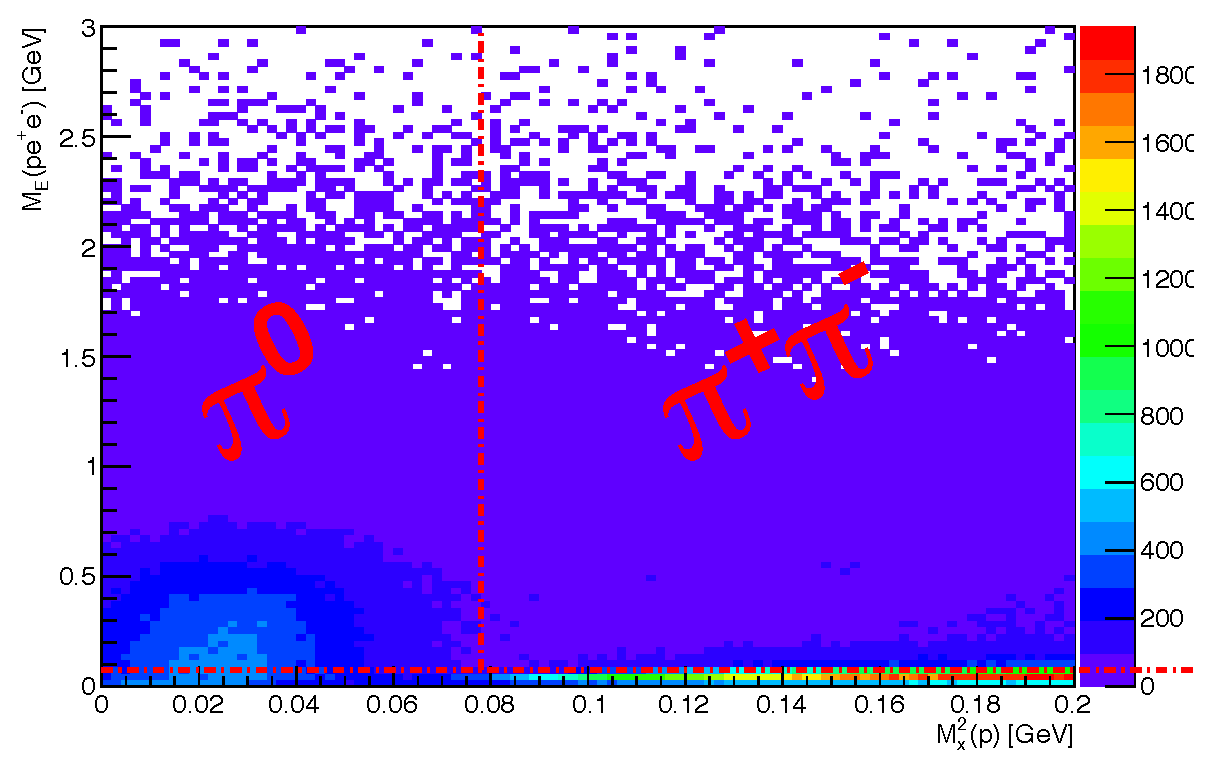
\includegraphics[width=0.6\textwidth]{figures/lepton/Lepfeature_cuts.eps}
\caption[Cuts Applied to Isolate \π[0] and \π[+]\π[-] for \abbr{PID} Validation]{\label{fig:islep.cuts}Plot of missing mass squared of off proton (horizontal) vs. missing energy of proton e$^+$e$^-$ (vertical). The red dashed vertical line depicts the $\π[+]\π[-]$ threshold mass cut while the horizontal red dashed line represents the missing energy cut-off used to sepertate $\π[+]\π[-]$ from \π[0].}
\end{center}\end{figure}

\subsubsection{\abbr{CC} Comparison}

The \abbr{NPE} measured by the \abbr{CC} for all positron/electron (e$^+$/e$^-$) candidates can be seen in Fig~\ref{fig:islep.CC}. The sharp decline prior to 2.5 \abbr{NPE} is due to photo-electrons created by electron/positrons, pions traveling through the \abbr{CC} or pions producing delta-electrons which pass through the \abbr{CC}. Delta-electrons are created as an effect of the ionization of gases that could be present when the pion travels through the \abbr{DC}. These types of electrons are typically lower in momentum than the electrons obtained from particle decays in \abbr{CLAS} and thus according to eq.~\ref{eq:cc.NPE} should emit less \abbr{NPE} per unit length.

Through mass conservation the particles for the \π[0] events must be e$^+$/e$^-$ pairs. In comparison to fig.~\ref{fig:islep.CC}, fig.~\ref{fig:islep.CC1} plots the \abbr{NPE} measured by the \abbr{CC} for all e$^+$/e$^-$ pairs for \π[0] events selected as shown in fig.~\ref{fig:islep.cuts}. It can be seen that the sharp decline prior to \abbr{NPE} = 2.5 is reduced leaving mostly electrons or positrons signatures in the \abbr{CC} concluding that the \desg{g7} \abbr{CC} \abbr{NPE} cut is valid for identifying e$^+$/e$^-$ pairs while rejecting \π[+]/\π[-] pairs.
 
%
\begin{figure}\begin{center}
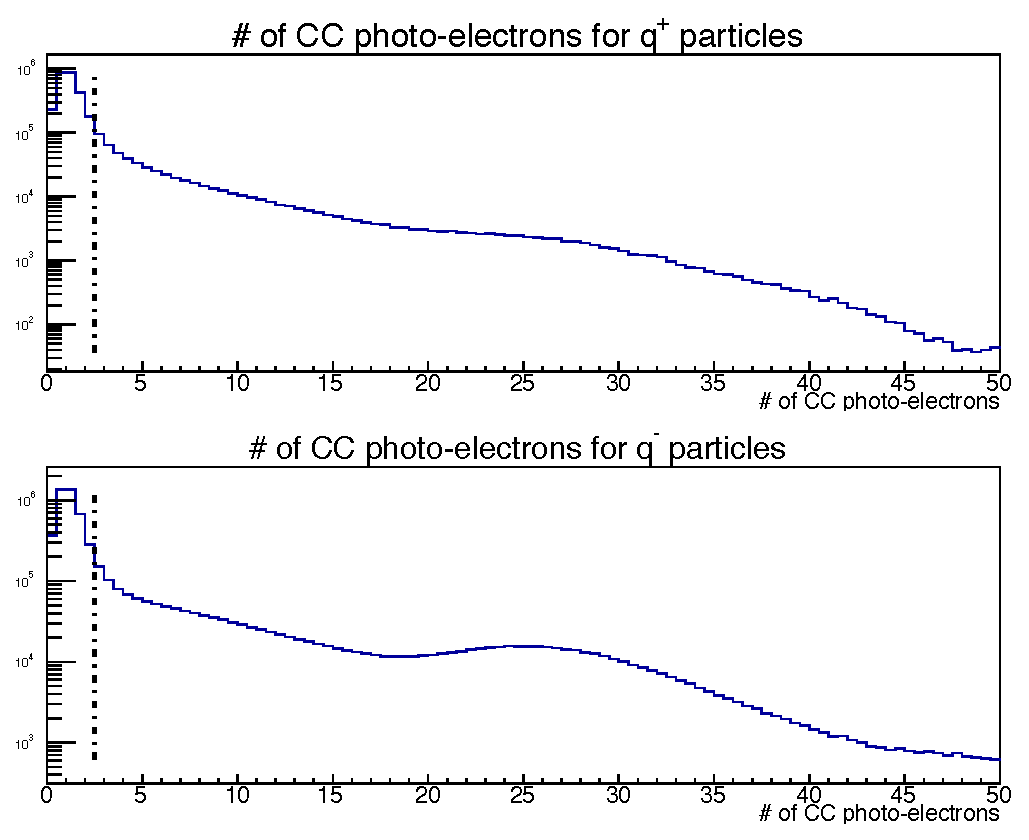
\includegraphics[width=0.6\textwidth]{figures/lepton/CC_nPE.eps}
\caption[Number of Photo-electrons Measured by \abbr{CC} for All e$^-$ and e$^+$ Candidates]{\label{fig:islep.CC}Plot of \abbr{NPE} measured by \abbr{CLAS} \abbr{CC} subsystem for positron/electron candidates top/bottom respectively. The dashed dotted vertical line depicts the cut applied if using the \desg{g7} lepton \abbr{PID} scheme.}
\end{center}\end{figure}

\begin{figure}\begin{center}
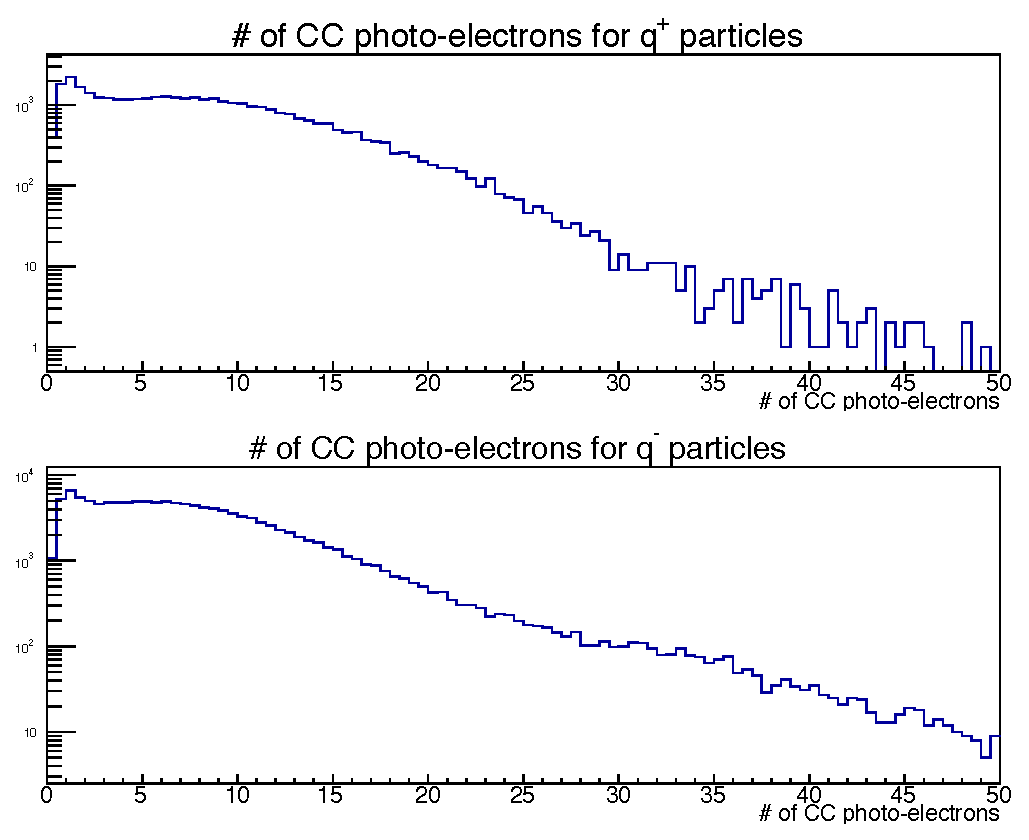
\includegraphics[width=0.6\textwidth]{figures/lepton/CC_NPEcut.eps}
\caption[Number of Photo-electrons Measured by \abbr{CC} for \π[0] Events]{\label{fig:islep.CC1}Plot of \abbr{NPE} measured by \abbr{CLAS} \abbr{CC} subsystem when selecting \π[0] events seen in Fig~\ref{fig:islep.cuts}, positron/electron candidates top/bottom respectively.}
\end{center}\end{figure}
\FloatBarrier
\subsubsection{\abbr{EC} Comparison}
%EC
%
%e-
%

Similarly to the \abbr{CC} comparison, figures~\ref{fig:islep.pimEClow},~\ref{fig:islep.pimEChigh},~\ref{fig:islep.pipEClow},~\ref{fig:islep.pipEChigh} depict the  p$\mathrm{_{thres}^{low}}$ and  p$\mathrm{_{thres}^{low}}$ cuts listed in  Table~\ref{tab:ISLEP_cuts} for the q$^-$ and q$^+$ tracks respectively. After \π[0] event selection, seen in figures~\ref{fig:islep.pimEC},~\ref{fig:islep.pimECcut} ,~\ref{fig:islep.pipEC} ,~\ref{fig:islep.pipECcut}, the bulk of e$^+$/e$^-$ events reside within the region of the cut acceptance therefore it is evident that the \desg{g7} \abbr{EC} cuts are valid for identifying e$^+$/e$^-$ pairs. The following four plots are for electron($e^-$) \abbr{PID} validation of the \desg{g7} \abbr{EC} cuts described in Table~\ref{tab:ISLEP_cuts}.
%
\begin{figure}\begin{center}
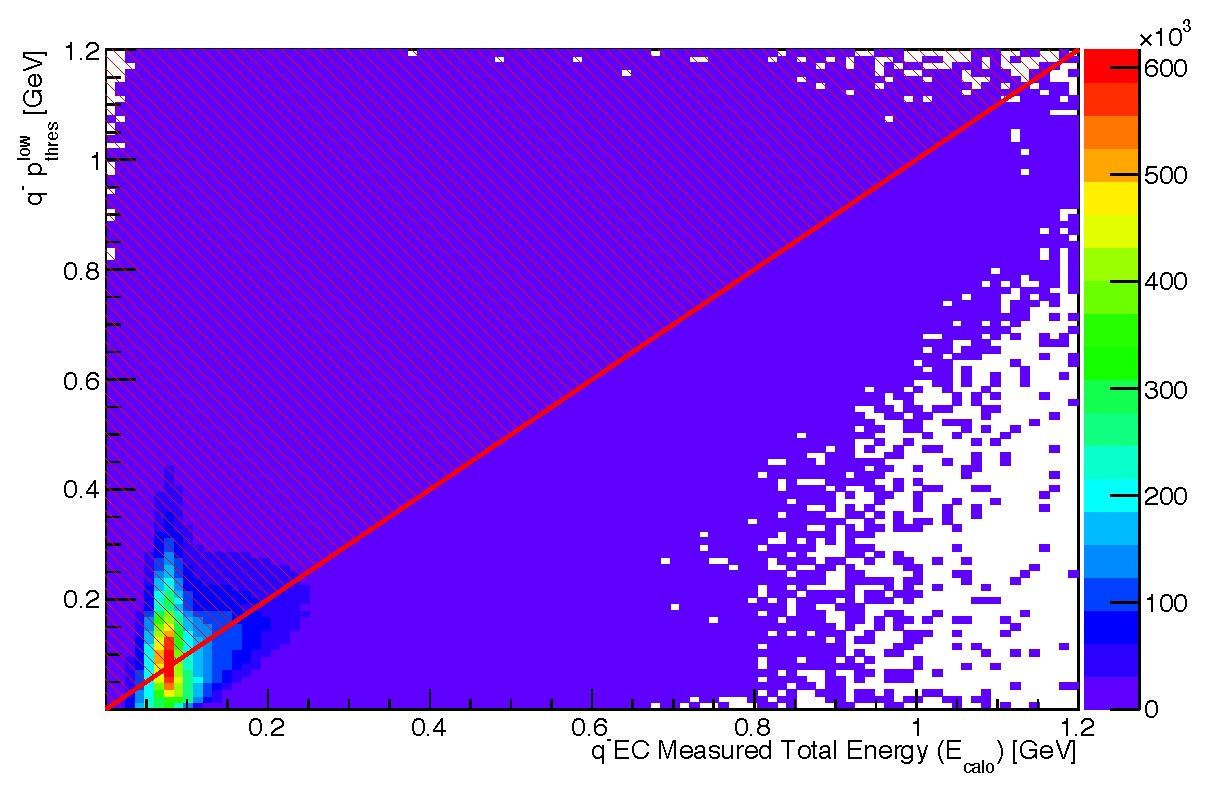
\includegraphics[width=0.6\textwidth]{figures/lepton/Pim_EClow.eps}
\caption[\abbr{EC} Deposited Energy Comparison to Lower Threshold Track Momentum for q$^-$ Tracks]{\label{fig:islep.pimEClow}Plot of energy deposited measured by \abbr{EC} vs. track momentum p$\mathrm{_{thres}^{low}}$ for negative charged tracks. The red region depicts the cut that would reject events in the \desg{g7} lepton \abbr{EC} \abbr{PID} scheme.}
\end{center}\end{figure}

\begin{figure}\begin{center}
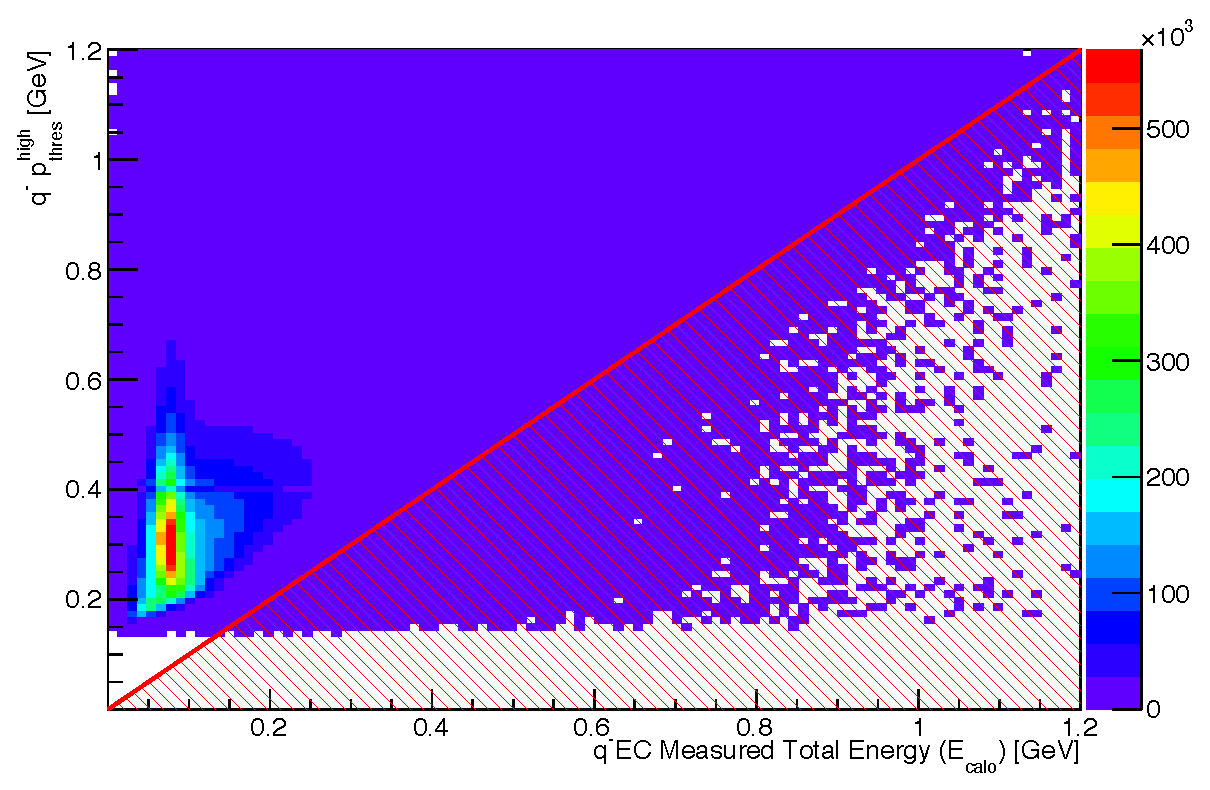
\includegraphics[width=0.6\textwidth]{figures/lepton/Pim_EChigh.eps}
\caption[\abbr{EC} Deposited Energy Comparison to Upper Threshold Track Momentum for q$^-$ Tracks]{\label{fig:islep.pimEChigh}Plot of energy deposited measured by \abbr{EC} vs. track momentum p$\mathrm{_{thres}^{high}}$ for negative charged tracks. The red region depicts the cut that would reject events in the \desg{g7} lepton \abbr{EC} \abbr{PID} scheme.}
\end{center}\end{figure}


\begin{figure}\begin{center}
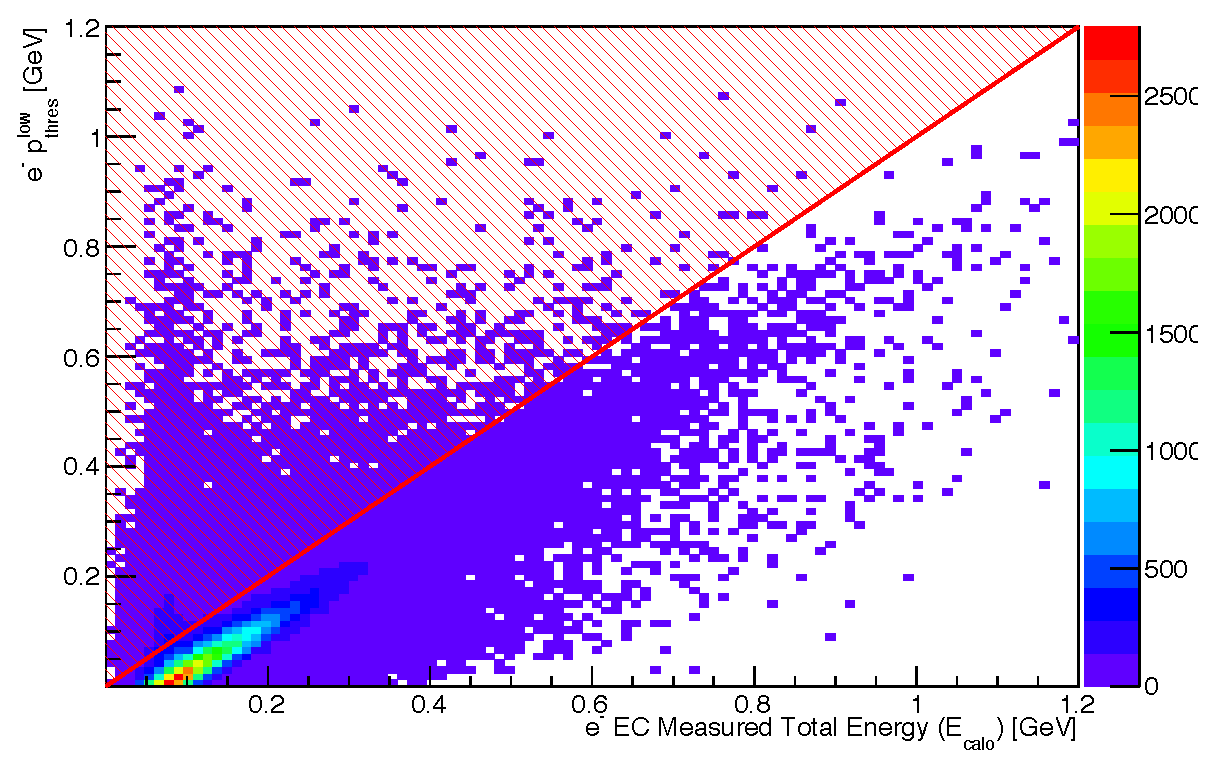
\includegraphics[width=0.6\textwidth]{figures/lepton/Pim_EClowcut.eps}
\caption[\abbr{EC} Deposited Energy Comparison to Track Momentum for e$^-$ Candidates]{\label{fig:islep.pimEC}Plot of energy deposited measured by \abbr{EC} vs. track momentum p$\mathrm{_{thres}^{low}}$ for electrons from \π[0] events without the \desg{g7} lepton \abbr{EC} \abbr{PID} scheme applied. The red region depicts the cut that would reject events in the \desg{g7} lepton \abbr{EC} \abbr{PID} scheme.}
\end{center}\end{figure}

\begin{figure}\begin{center}
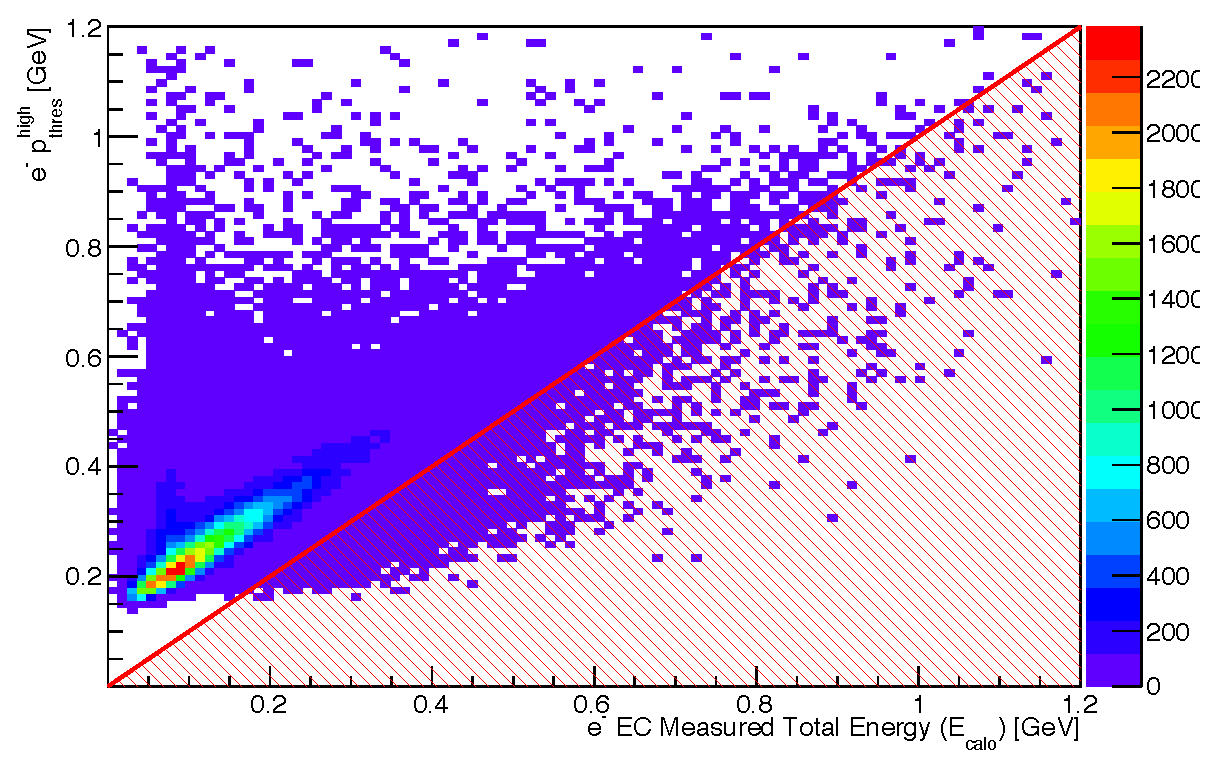
\includegraphics[width=0.6\textwidth]{figures/lepton/Pim_EChighcut.eps}
\caption[\abbr{EC} Deposited Energy Comparison to Track Momentum for e$^-$ from \π[0] Events]{\label{fig:islep.pimECcut}Plot of energy deposited measured by \abbr{EC} vs. track momentum p$\mathrm{_{thres}^{high}}$ for electrons from \π[0] events without the \desg{g7} lepton \abbr{EC} \abbr{PID} scheme applied. The red region depicts the cut that would reject events in the \desg{g7} lepton \abbr{EC} \abbr{PID} scheme.}
\end{center}\end{figure}
\FloatBarrier
The following four plots are for positron($e^+$) \abbr{PID} validation of the \desg{g7} \abbr{EC}
cuts described in Table~\ref{tab:ISLEP_cuts}.
%
%
%e+
%
%
\begin{figure}\begin{center}
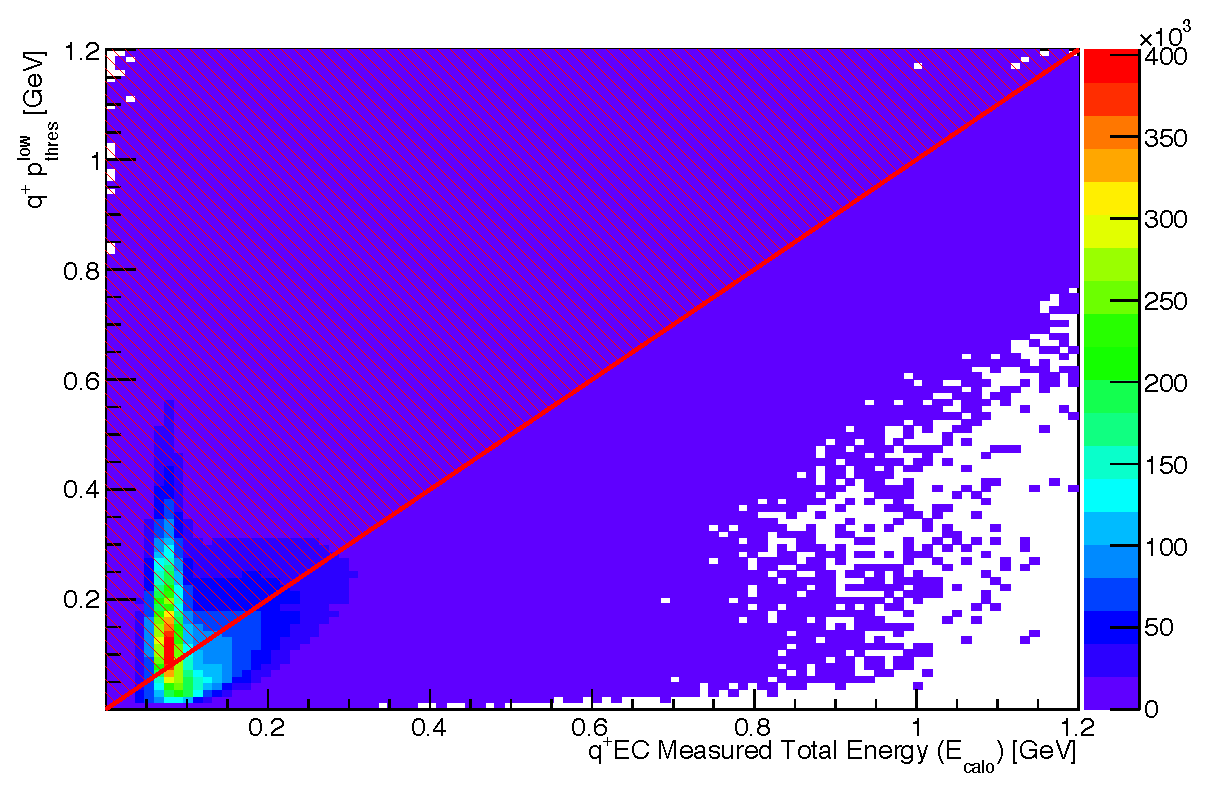
\includegraphics[width=0.9\columnwidth]{figures/lepton/Pip_EClow.eps}
\caption[\abbr{EC} Deposited Energy Comparison to Lower Threshold Track Momentum for q$^+$ Tracks]{\label{fig:islep.pipEClow}Plot of energy deposited measured by \abbr{EC} vs. track momentum p$\mathrm{_{thres}^{low}}$ for positive charged tracks. The red region depicts the cut that would reject events in the \desg{g7} lepton \abbr{EC} \abbr{PID} scheme.}
\end{center}\end{figure}

\begin{figure}\begin{center}
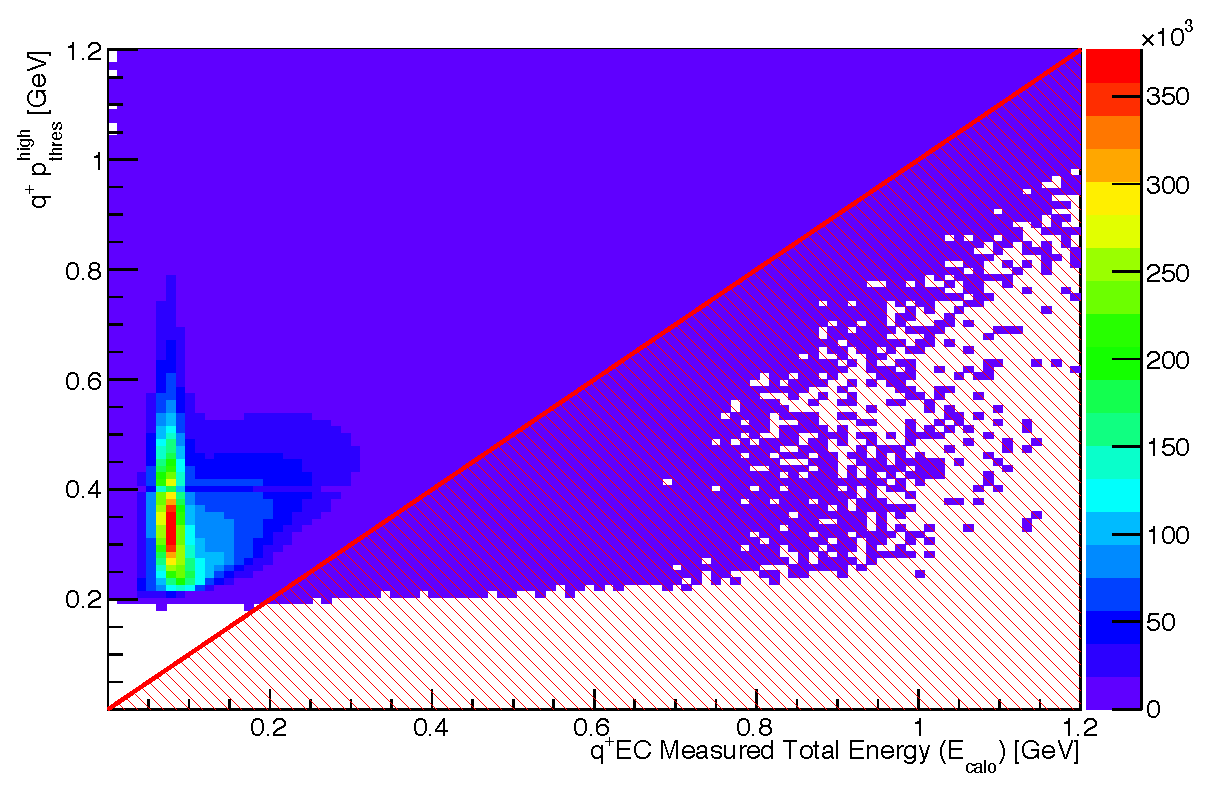
\includegraphics[width=0.9\columnwidth]{figures/lepton/Pip_EChigh.eps}
\caption[\abbr{EC} Deposited Energy Comparison to Upper Threshold Track Momentum for q$^+$ Tracks]{\label{fig:islep.pipEChigh}Plot of energy deposited measured by \abbr{EC} vs. track momentum p$\mathrm{_{thres}^{high}}$ for positive charged tracks. The red region depicts the cut that would reject events in the \desg{g7} lepton \abbr{EC} \abbr{PID} scheme.}
\end{center}\end{figure}

\begin{figure}\begin{center}
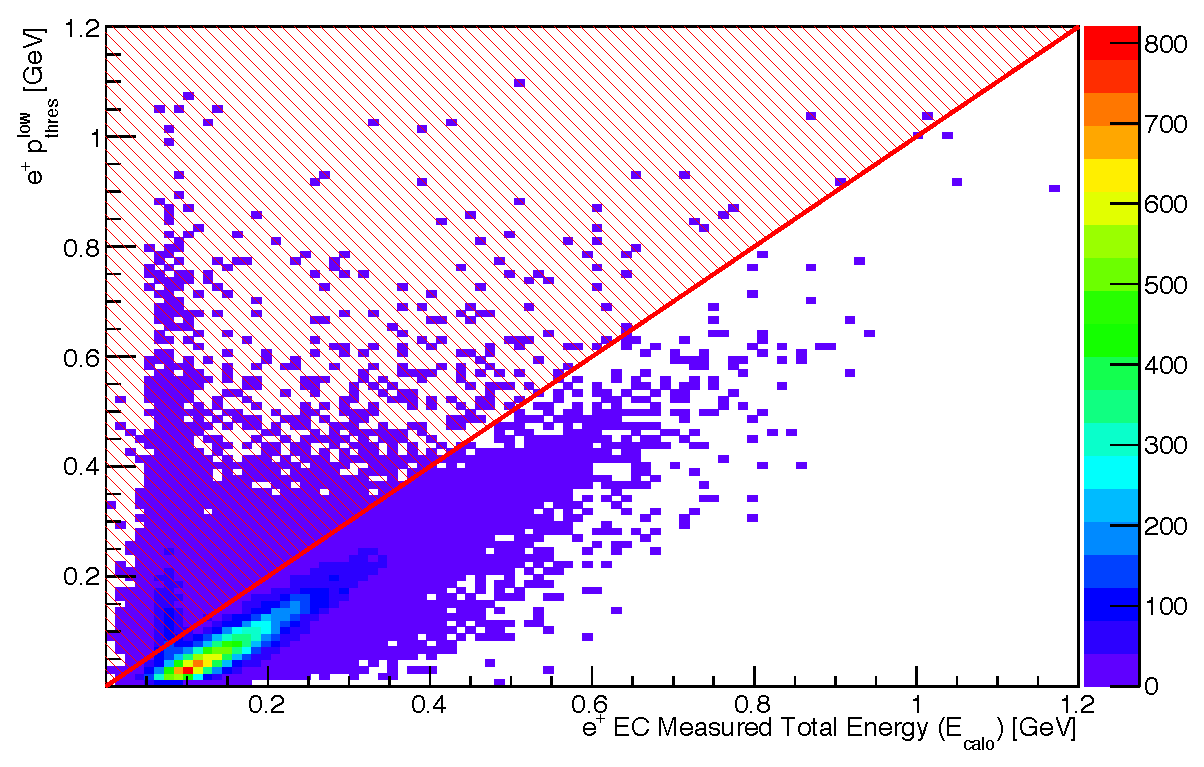
\includegraphics[width=0.9\columnwidth]{figures/lepton/Pip_EClowcut.eps}
\caption[\abbr{EC} Deposited Energy Comparison to Track Momentum for e$^+$ Candidates]{\label{fig:islep.pipEC}Plot of energy deposited measured by \abbr{EC} vs. track momentum p$\mathrm{_{thres}^{low}}$ for positrons from \π[0] events without the \desg{g7} lepton \abbr{EC} \abbr{PID} scheme applied. The red region depicts the cut that would reject events in the \desg{g7} lepton \abbr{EC} \abbr{PID} scheme.}
\end{center}\end{figure}

\begin{figure}\begin{center}
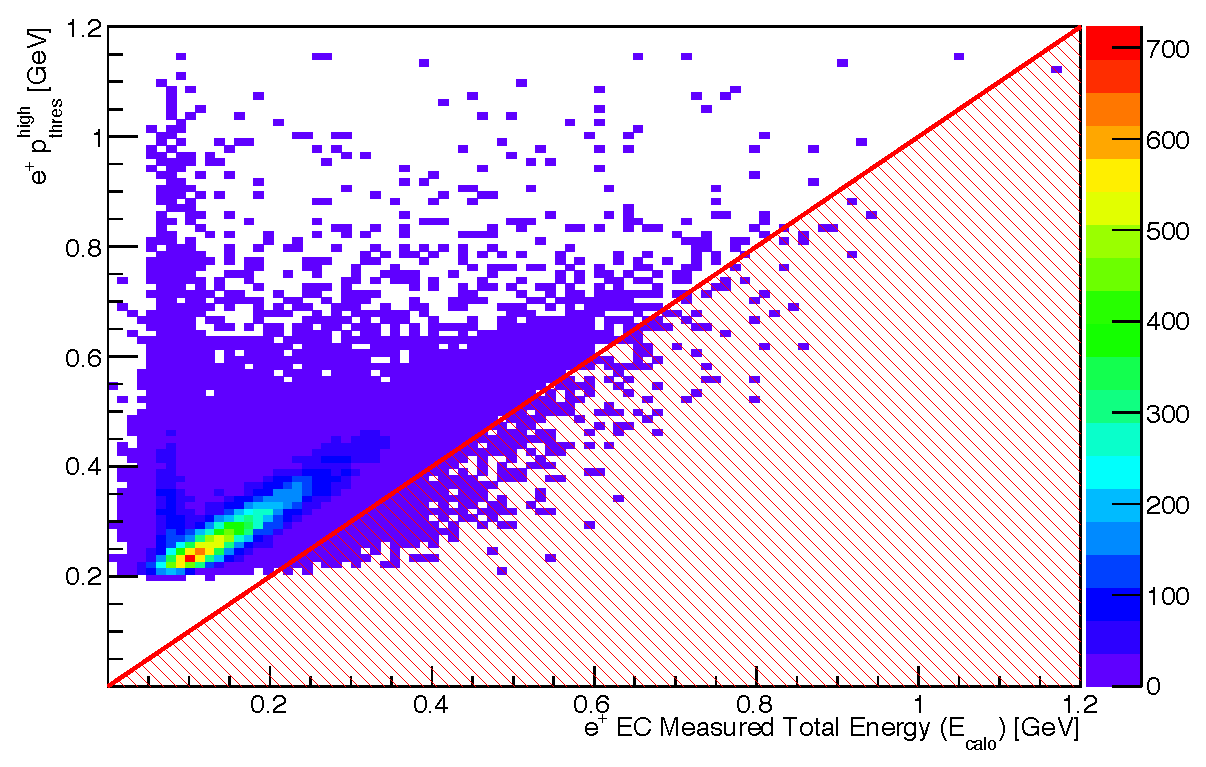
\includegraphics[width=0.9\columnwidth]{figures/lepton/Pip_EChighcut.eps}
\caption[\abbr{EC} Deposited Energy Comparison to Track Momentum for e$^+$ from \π[0] Events]{\label{fig:islep.pipECcut}Plot of energy deposited measured by \abbr{EC} vs. track momentum p$\mathrm{_{thres}^{high}}$ for positrons from \π[0] events without the \desg{g7} lepton \abbr{EC} \abbr{PID} scheme applied. The red region depicts the cut that would reject events in the \desg{g7} lepton \abbr{EC} \abbr{PID} scheme.}
\end{center}\end{figure}
%


\FloatBarrier



\begin{singlespacing}

\clearpage
\phantomsection \addcontentsline{toc}{section}{References}

\printbibliography

%\clearpage
%\phantomsection \addcontentsline{toc}{chapter}{Index}
%\printindex

\end{singlespacing}

\end{document}
